% file: HrdwCCppCUDA_grande.tex
% Computational Physics (notes), in unconventional ``grande'' format; fitting a widescreen format
% 
% github        : ernestyalumni
% gmail         : ernestyalumni 
% linkedin      : ernestyalumni 
% wordpress.com : ernestyalumni
%
% This code is open-source, governed by the Creative Common license.  Use of this code is governed by the Caltech Honor Code: ``No member of the Caltech community shall take unfair advantage of any other member of the Caltech community.'' 

\documentclass[10pt]{amsart}
\pdfoutput=1
%\usepackage{mathtools,amssymb,lipsum,caption}
\usepackage{mathtools,amssymb,caption}


\usepackage{graphicx}
\usepackage{hyperref}
\usepackage[utf8]{inputenc}
\usepackage{listings}
\usepackage[table]{xcolor}
\usepackage{pdfpages}
\usepackage{tikz}
\usetikzlibrary{graphs,matrix,arrows, positioning, shapes}

\usepackage{multicol}

\hypersetup{colorlinks=true,citecolor=[rgb]{0,0.4,0}}

\oddsidemargin=15pt
\evensidemargin=5pt
\hoffset-45pt
\voffset-55pt
\topmargin=-4pt
\headsep=5pt
\textwidth=1120pt
\textheight=595pt
\paperwidth=1200pt
\paperheight=700pt
\footskip=40pt


\newtheorem{theorem}{Theorem}
\newtheorem{corollary}{Corollary}
%\newtheorem*{main}{Main Theorem}
\newtheorem{lemma}{Lemma}
\newtheorem{proposition}{Proposition}

\newtheorem{definition}{Definition}
\newtheorem{remark}{Remark}

\newenvironment{claim}[1]{\par\noindent\underline{Claim:}\space#1}{}
\newenvironment{claimproof}[1]{\par\noindent\underline{Proof:}\space#1}{\hfill $\blacksquare$}

%This defines a new command \questionhead which takes one argument and
%prints out Question #. with some space.
\newcommand{\questionhead}[1]
  {\bigskip\bigskip
   \noindent{\small\bf Question #1.}
   \bigskip}

\newcommand{\problemhead}[1]
  {
   \noindent{\small\bf Problem #1.}
   }

\newcommand{\exercisehead}[1]
  { \smallskip
   \noindent{\small\bf Exercise #1.}
  }

\newcommand{\solutionhead}[1]
  {
   \noindent{\small\bf Solution #1.}
   }


  \title[Hardware (Compilers, OS, runtime) and C, C++, to CUDA]{Hardware (Compilers, OS, runtime) and C, C++, to CUDA}
\author{Ernest Yeung \href{mailto:ernestyalumni@gmail.com}{ernestyalumni@gmail.com}}
\date{1 Nov 2017}
\keywords{C, C++, CUDA, CUDA C/C++, Compilers, OS, runtime, classes, Object Oriented Programming, Segmentation Fault, memory, memory addresses}

\begin{document}

\definecolor{darkgreen}{rgb}{0,0.4,0}
\lstset{language=C++,
  keywordstyle=\color{blue},
  stringstyle=\color{red},
 commentstyle=\color{darkgreen}
 }
%\lstlistoflistings

\maketitle

\tableofcontents


\begin{multicols*}{2}

\begin{abstract}
I review what, how, and why Segmentation Fault is and occurs in the specific context of C and hopefully to CUDA, virtual memory addresses in C++, and to CUDA.  


\end{abstract}

\section{Introduction; why I'm writing this}  

I didn't realize the importance of having a profound understanding of C/C++ and its relation to hardware, in particular memory (addresses), until I learned more specifically about the work done at NVIDIA from its news and job postings.  Coming from a theoretical and mathematical physics background, I wanted to get myself up to speed as fast as possible, provide good textbook and online references, and directly relate these topics, which seem to be classic topics in computer science (at hardware level) and electrical engineering, to CUDA, to specifically GPU parallel programming with direct CUDA examples.  

Note that there is a version of this LaTeX/pdf file in the usual "letter" format that is exactly the same as the content here, \verb|HrdwCCppCUDA.pdf|.  

Meyer (1997) \cite{Meye1997}


\begin{quotation}
"When programmers first began giving up assembly language in favor of using HLLs, they generally understood the low-level ramifications of the HLL statements they were using and could choose their HLL statements appropriately.Unfortunately, the generation of computer programmers that followed them did not have the benefit of mastering assembly language. As such, they were not in a position to wisely choose statements and data structures that HLLs could efficiently translate into machine code."  
\end{quotation}
pp. 2, Ch. 1 of Hyde (2006) \cite{Hyde2006}, where HLL stands for high-level language.  I was part of that generation and knew of nothing of assembly.  


Bryant and O'Hallaron (2015) \cite{BrOH2016}

\section{How Computers Store Data}

"How Computers Store Data" in \emph{Data Structures: Introduction}, Neagole (2020) \cite{Neag2020}

Persistent storage is slow. \\
CPU needs access to RAM and storage. CPU can access RAM a lot faster. \\
When a variable is declared, it'll hold value in memory RAM. \\
CPU grabs program in storage. To run fast, hold variable in RAM. \\ 
Think of RAM as massive storage area with numbered shelves - \emph{addresses}. Each address holds 8 bits $=$ 1 byte. \\
CPU is connected to a memory controller, and memory controller does actual reading of RAM memory, as well as writing to this memory. \\
When CPU asks what's at this address? memory controller actually has individual connections to each address; this is important, it means we can access 0th address and immediately access 7th address, or Nth address, thus RAM - random access memory - memory controller can jump to any address, but closer information is to CPU, less time to travel. \\
CPU cache- where CPU stores on tiny memory a copy of recent data; e.g. LRU cache.

Store variable \verb|var a = 1| in "word" ("block") 32-bit, store next varaible in next block. \\
overflow (TODO: review overflow implementation). \\
Some data structures are organized in consecutive addresses, some apart.

\section{80x86 Assembly; 80x86 Architecture}  

cf. Ch. 3 of Hyde (2006) \cite{Hyde2006}

Main difference between complex instruction set computer (CISC) architectures such as 80x86 and reduced instruction set computer (RISC) architectures like PowerPC is the way they use memory.  RISC provde relatively clumsy memory access, and applications avoid accessing memory.  80x86 access memory in many different ways and applications take advantage of these facilities.  

\subsection{Basic 80x86 Architecture}  

Intel CPU generally classified as a \emph{Von Neumann machine}, containing 3 main building blocks:
\begin{enumerate}
	\item CPU
	\item memory
	\item input/output (I/O) devices
\end{enumerate}
These 3 components are connected together using the \emph{system bus}.  System bus consists of 
\begin{itemize}
	\item address bus
	\item data bus
	\item control bus
\end{itemize}

CPU communicates with memory and I/O devices by placing a numeric value on the address bus to select 1 of the memory locations or I/O device port locations, each of which has a unique binary numeric address.   \\
Then the CPU, I/O, and memory devices pass data among themselves by placing data on the data bus.   \\
Control bus contains signals that determine the direction of data transfer (to or from memory, and to or from an I/O device).  

So 
\[
\begin{gathered}
\begin{gathered}
\textbf{Memory} \\
\text{Obj}{(\textbf{Memory})} = \text{ memory locations } 
\end{gathered} \\ 
\begin{gathered}
\textbf{I/O} \\
\text{Obj}{(\textbf{I/O})} = \text{ I/O device port locations } 
\end{gathered}
\end{gathered}
\]
and 
\[
\begin{gathered}
\textbf{address bus} \\
\text{Obj}{(\textbf{address bus})} = \text{ unique binary numeric addresses } 
\end{gathered}
\]

Likewise, 
\[
\begin{gathered}
\textbf{data bus} \\
\text{Obj}{(\textbf{data bus})} = \text{ data } 
\end{gathered}
\]

And so
\[
\begin{gathered}
\text{CPU} : \textbf{Memory} \times \textbf{address bus} \to \text{Hom}{(\textbf{Memory} , \textbf{address bus}) } \\ 
	\text{CPU}: (\text{memory location} , \text{unique binary numeric address}) \mapsto \&
\end{gathered}
\]
in the language of category theory.  

\subsection{Registers (for 80x86)}  

cf. 3.3 Basic 80x86 Architecture, from pp. 23 of Hyde (2006) \cite{Hyde2006}.  

Example: to add 2 variables, $x,y$ and store $x+y$ into $z$, you must load 1 of the variables into a register, add the 2nd. operand to the register, and then store register's value into destination variable.  "Registers are middlemen in almost every calculation." Hyde (2006) \cite{Hyde2006}.  
    

 There are 4 categories of 80x86 CPU registers: 
 \begin{itemize}
 	\item general-purpose
 	\item special-purpose application-accessible
 	\item segment
 	\item special-purpose kernel-mode
 \end{itemize}
Segment registers not used very much in modern 32-bit operating systems (e.g. Windows, Linux; what about 64-bit?) and special-purpose kernel-mode registers are intended for writing operating systems, debuggers, and other system-level tools.  

\subsubsection{80x86 General-Purpose Registers}  

80x86 CPUs provide several general-purpose registers, including 8 32-bit registers having the following names: (8 bits in 1 byte, 32-bit is 4 bytes)

\[
EAX, EBX, ECX, EDX, ESI, EDI, EBP, ESP
\]
where E is \emph{extended}; 32-bit registers distinguished from 8 16-bit registers with following names 

\[
AX, BX, CX, DX, SI, DI, BP, SP
\]
and finally 

\[
AL, AH, BL, BH, CL, CH, DL, DH
\]
Hyde says that it's important to note about the general-purpose registers is they're not independent.  80x86 doesn't provide 24 separate registers, but overlaps the 32-bit registers with 16-bit registers, and overlaps 16-bit registers with 8-bit registers.  e.g.

\[
\begin{gathered}
\&AL \neq \&AH, \text{ but } \\
\&AL, \&AH \in \&AX \text{and } \&AX \in \&EAX, \text{ so that } \\
\&AL , \&AH, \&AX \in \&EAX
\end{gathered}
\]

\section{Compilers; Compiler Operation and Code Generation}

cf. Ch. 5 Compiler Operation and Code Generation, from pp. 62 and pp. 72- of Hyde (2006) \cite{Hyde2006}


\section{gdp; good debugging processes (in C/C++/CUDA)}

\href{https://youtu.be/heEaKf2b1uA}{Learn C the hard way Lecture 4, Using Debugger (GDB) }


\section{Pointers in C; Pointers in C categorified (interpreted in Category Theory) and its relation to actual, physical, computer memory and (memory) addresses ((address) bus; pointers, structs, arrays in C}

From Shaw (2015) \cite{Shaw2015}, Exercise 15, 

e.g. \verb|ages[i]|, You're indexing into array \verb|ages|, and you're using the number that's held in $i$ to do it:  
\[
\begin{aligned}
& a : \mathbb{Z} \to \text{Type} \in \textbf{Type}  \\
& a: i \mapsto a[i]
\end{aligned} \text{ e.g. } 
\begin{aligned}
& a: \mathbb{Z} \to \mathbb{R} \text{ or } \mathbb{Z}  \\
& a:i \mapsto a[i]
\end{aligned}
\]

Index $i\in \mathbb{Z}$ is a location \emph{inside} \verb|ages| or $a$, which can also be called \emph{address}.  Thus, $a[i]$.  

Indeed, from \href{http://en.cppreference.com/w/cpp/language/operator_member_access}{cppreference for Member access operators}, 

Built-in \emph{subscript} operator provides access to an object pointed-to by pointer or array operand.  And so \verb|E1[E2]| is exactly identical to \verb|*(E1+E2)|.  


To C, e.g. \verb|ages|, or $a$, is a location in computer's memory where, e.g., all these integers (of \verb|ages|) start, i.e. where $a$ starts.  

\[
\begin{aligned}
& \textbf{Memory} , \qquad \, \text{Obj}{(\textbf{Memory})} \ni \text{ memory location.  Also, to specify CPU, } \\ 
& \textbf{Memory}_{CPU} , \qquad \, \text{Obj}{(\textbf{Memory}_{CPU})} \ni \text{ computer memory location }
\end{aligned}
\]

It's \emph{also} an address, and C compiler will replace e.g. \verb|ages| or array $a$, anywhere you type it, with address of very 1st integer (or 1st element) in, e.g. \verb|ages|, or array $a$.  

\[
\begin{gathered}
\begin{aligned}
\textbf{Arrays} & \xleftrightarrow{ \cong } \textbf{address}  \\
\text{Obj}{(\textbf{Arrays} )} & \xleftrightarrow{ \cong } \text{Obj}{(\textbf{address} )}  \\
a & \xleftrightarrow{ \cong } \verb|0x17|  \\
\end{aligned}
\end{gathered}
\]

"But here's the trick": e.g. "\verb|ages| is an address inside the \emph{entire computer}." (Shaw (2015) \cite{Shaw2015}).  

It's not like $i$ that's just an address inside \verb|ages|.  \verb|ages| array name is actually an address in the computer.     

"This leads to a certain realization: C thinks your whole computer is 1 massive array of bytes."  

"What C does is layer on top of this massive array of bytes the concept of types and sizes of those types." (Shaw (2015) \cite{Shaw2015}).  


Let 
\[
\begin{gathered}
\begin{aligned}
& \textbf{Memory}_{CPU} := 1 \text{ massive array of bytes } \\
& \text{Obj}{(\textbf{Memory}_{CPU})} 
\end{aligned}  \qquad \, \qquad \, 
\begin{aligned}
& \textbf{Type} \\
& \text{Obj}{(\textbf{Type})} \ni \verb|int|, \verb|char|, \verb|float| \\
& \text{Obj}{(\textbf{Type})}  \xrightarrow{\texttt{sizeof}} \mathbb{Z}^+  \\
& T \xmapsto{ \texttt{sizeof} } \verb|sizeof|(T) \\
& \verb|float| \xmapsto{ \texttt{sizeof}} \verb|sizeof|(\verb|float|)
\end{aligned}
\end{gathered}
\]


How C is doing the following with your arrays:  

\begin{itemize}
	\item \emph{Create} a block of memory inside your computer:  
	\[
	\text{Obj}{(\textbf{Memory}_{CPU})} \supset \text{ Memory block }  
	\]
	Let $\text{Obj}{(\textbf{Memory}_{CPU})}$ be an ordered set.  Clearly, then memory can be indexed.  Let $b\in \mathbb{Z}^+$ be this index.  Then Memory block(0) $= \text{Obj}{(\textbf{Memory}_{CPU})}(b)$.  		
	\item \emph{Pointing} the name \verb|ages|, or $a$, to beginning of that (memory) block.  
	
	Entertain, possibly, a category of pointers, $\textbf{Pointers} \equiv \textbf{ptrs}$.  
	\[
	\begin{gathered}
	\textbf{ptrs} \\
	\text{Obj}{(\textbf{ptrs})} \ni a, \text{ e.g. } \verb|ages|  
	\end{gathered}
	\]	
	\[
	\begin{gathered}
	a \mapsto \text{Memory block}(0) \\ 
	\text{Obj}{(\textbf{ptrs})} \to \text{Obj}{(\textbf{Memory}_{CPU})}
	\end{gathered}
	\]
	\item \emph{indexing} into the block, by taking the base address of \verb|ages|, or $a$ 
\end{itemize}

\[
\begin{gathered}
\begin{aligned}
&	a \xmapsto{ \cong } \text{ base address $0x17$ } \\
&	\text{Obj}{((T)\textbf{array})} \xrightarrow{ \cong } \text{Obj}{(\textbf{addresses})}  \\	
&	a[i] \equiv a+i \xmapsto{ \cong } \text{ base address + i * } \verb|sizeof|(T)  \xmapsto{ * } a[i] \in T \text{ where $T$, e.g. $T = \mathbb{Z},\mathbb{R}$ } \\ 
& \text{Obj}{((T)\textbf{array}} \xrightarrow{ \cong } \text{Obj}{(\textbf{addresses})} \to T  
\end{aligned}
\end{gathered}
\]

"A pointer is simply an address pointing somewhere inside computer's memory with a type specifier."  Shaw (2015) \cite{Shaw2015}


C knows where pointers are pointing, data type they point at, size of those types, and how to get the data for you.  

\subsubsection{Practical Pointer Usage}
\begin{itemize}
	\item Ask OS for memory block (chunk of memory) and use pointer to work with it.  This includes strings and \verb|structs|.  
	\item Pass by reference - pass large memory blocks (like large structs) to functions with a pointer, so you don't have to pass the entire thing to the function.  
	\item Take the address of a function, for dynamic callback. (function of functions)
\end{itemize}

"You should go with arrays whenever you can, and then only use pointers as performance optimization if you absolutely have to."  Shaw (2015) \cite{Shaw2015}

\subsubsection{Pointers are not Arrays}  

No matter what, pointers and arrays are not the same thing, even though C lets you work with them in many of the same ways.  

From Eli Bendersky's website, \href{https://eli.thegreenplace.net/2009/10/21/are-pointers-and-arrays-equivalent-in-c}{Are pointers and arrays equivalent in C?}

He also emphasizes that 

\subsubsection{Variable names in C are just labels}  

"A variable in C is just a convenient, alphanumeric pseudonym of a memory location." (Bendersky, \cite{Bend}).  What a compiler does is, create label in some memory location, and then access this label instead of always hardcoding the memory value.   

"Well, actually the address is not hard-coded in an absolute way because of loading and relocation issues, but for the sake of this discussion we don't have to get into these details." (Bendersky, \cite{Bend}) (EY : 20171109 so it's on the address bus?)

Compiler assigns label \emph{at compile time}.  Thus, the great difference between arrays and pointers in C.  

\subsubsection{Arrays passed to functions are converted to pointers}  

cf. Bendersky, \cite{Bend}.  

Arrays passed into functions are always converted into pointers.  The argument declaration \verb|char arr_place[]| in  

\begin{lstlisting}
void foo(char arr_arg[], char* ptr_arg)
{
	char a = arr_arg[7];
	char b = ptr_arg[7];
}
\end{lstlisting} 

is just syntactic sugar to stand for \verb|char* arr_place|.  

From Kernighan and Ritchie (1988) \cite{KeRi1988}, pp. 99 of Sec. 5.3, Ch. 5 Pointers and Arrays,  

\begin{quotation}
	When an array name is passed to a function, what is passed is the location of the initial element.  Within the called function, this argument is a local variable, and so an array name parameter is a pointer, that is, a variable containing an address.  
	\end{quotation}

Why?  

The C compiler has no choice here, since, \\
array name is a label the C compiler replaces \emph{at compile time}  with the address it represents (which for arrays is the address of the 1st element of the array).  

But function isn't called at compile time; it's called \emph{at run time}.  \\
At run time, (where) something should be placed on the stack to be considered as an argument.  

Compiler cannot treat array references inside a function as labels and replace them with addresses, because it has no idea what actual array will be passed in at run time.  

EY : 20171109 It can't anticipate the exact arguments that'll it be given \emph{at run-time}; at the very least, my guess is, it's given instructions.  

Bendersky \cite{Bend} concludes by saying the difference between arrays and pointers does affect you.  One way is how arrays can't be manipulated the way pointers can.  Pointer arithmetic isn't allowed for arrays and assignment to an array of a pointer isn't allowed.  cf. van der Linden (1994) \cite{Vand1994}. Ch. 4, 9, 10.  

Bendersky \cite{Bend} has this one difference example, "actually a common C gotcha":  

"Suppose one file contains a global array:"  

\begin{lstlisting}
char my_Arr[256]  
\end{lstlisting}

Programmer wants to use it in another file, \emph{mistakingly} declares as  
\begin{lstlisting}
extern char* my_arr; 
\end{lstlisting}

When he tries to access some element of the array using this pointer, he'll most likely get a segmentation fault or a fatal exception (nomenclature is OS-dependent).  

To understand why, Bendersky \cite{Bend} gave this hint:  look at the assembly listing  

\begin{lstlisting}
    char a = array_place[7];

0041137E  mov  al,byte ptr [_array_place+7 (417007h)]
00411383  mov  byte ptr [a],al

char b = ptr_place[7];

00411386  mov  eax,dword ptr [_ptr_place (417064h)]
0041138B  mov  cl,byte ptr [eax+7]
0041138E  mov  byte ptr [b],cl
\end{lstlisting}

or my own, generated from \verb|gdb| on Fedora 25 Workstation Linux:

\begin{lstlisting}
0x00000000004004b1 <main+11>:	movzbl 0x200b8f(%rip),%eax        # 0x601047 <array_place+7>
0x00000000004004b8 <main+18>:	mov    %al,-0x1(%rbp)

0x00000000004004bb <main+21>:	mov    0x200be6(%rip),%rax        # 0x6010a8 <ptr_place>
0x00000000004004c2 <main+28>:	movzbl 0x7(%rax),%eax
0x00000000004004c6 <main+32>:	mov    %al,-0x2(%rbp)
\end{lstlisting}

"How will the element be accessed via the pointer?  What's going to happen if it's not actually a pointer but an array?"  Bendersky \cite{Bend}   

EY : 20171106.  Instruction-level, the pointer has to     
\begin{itemize}
	\item \verb|mov    0x200be6(%rip),%rax| - 1st., copy value of the pointer (which holds an address), into \verb|%rax| register.  
	\item \verb|movzbl 0x7(%rax),%eax| - off that address in register `%rax`, offset by 7 (or whatever the offset would be) and get value ther with \verb|%eax| register/instruction  
	\item \verb|mov    %al,-0x2(%rbp)| - \verb|mov| contents \verb|-0x2(%rbp)|into register \verb|%al|
\end{itemize}

If it's not actually a pointer, but an array, the value is copied into the \verb|%rax| register is an actual \verb|char| (or \verb|float|, some type).  \emph{Not} an address that the registers may have been expecting!  

\subsection{Structs in C}
From Shaw (2015) \cite{Shaw2015}, Exercise 16, 

\verb|struct| in C is a collection of other data types (variables) that are stored in 1 block of memory.  You can access each variable independently by name.  

\begin{itemize}
	\item The \verb|struct| you make, i.e.g \verb|struct Person| is now a \emph{compound data type}, meaning you can refer to \verb|struct Person| using the same kinds of expressions you would for other (data) types.
	\item This lets you pass the whole \verb|struct| to other functions
	\item You can access individual members of \verb|struct| by their names using \verb|x->y| if dealing with a ptr.  
\end{itemize}  

If you didn't have \verb|struct|, you'd have to figure out the size, packing, and location of memory of the contents.  In C, you'd let it handle the memory structure and structuring of these compound data types, \verb|struct|s.  (Shaw (2015) \cite{Shaw2015})



\part{C, Stack, Heap Memory Management in C}

\section{C, Stack and Heap Memory Management, Heap and Stack Memory Allocation}  

cf. Ex. 17 of Shaw (2015) \cite{Shaw2015}

Consider chunk of RAM called stack, another chunk of RAM called heap.  Difference between heap and stack depends on where you get the storage.  

Heap is all the remaining memory on computer.  Access it with \verb|malloc| to get more.  \\
Each time you call \verb|malloc|, the OS uses internal functions (EY : 20171110 address bus or overall system bus?) to register that piece of memory to you, then returns ptr to it.  

When done, use \verb|free| to return it to OS so OS can use it for other programs.  Failing to do so will cause program to \emph{leak} memory.  (EY: 20171110, meaning this memory is unavailable to the OS?)

Stack, on a special region of memory, stores temporary variables, which each function creates as locals to that function.  How stack works is that each argument to function is \emph{pushed} onto stack and then used inside the function.  Stack is really a stack data structure, LIFO (last in, first out).  This also happens with all local variables in \verb|main|, such as \verb|char action|, \verb|int id|.  The advantage of using stack is when function exits, \emph{C compiler} pops these variables off of stack to clean up.  

Shaw's mantra: If you didn't get it from \verb|malloc|, or a function that got it from \verb|malloc|, then it's on the stack.  

3 primary problems with stacks and heaps: 
\begin{itemize}
	\item If you get a memory block from \verb|malloc|, and have that ptr on the stack, then when function exits, ptr will get popped off and lost.  
	\item If you put too much data on the stack (like large structs and arrays), then you can cause a \emph{stack overflow} and program will abort.  Use the heap with \verb|malloc|.  
	\item If you take a ptr, to something on stack, and then pass or return it from your function, then the function receiving it will \emph{segmentation fault}, because actual data will get popped off and disappear.  You'll be pointing at dead space.  
\end{itemize}
cf. Ex. 17 of Shaw (2015) \cite{Shaw2015}

\section{Data segments; Towards Segmentation Fault}

cf. Ferres (2010) \cite{Ferr2010}

When program is loaded into memory, it's organized into 3 \emph{segments} (3 areas of memory):  
let executable program generated by a compiler (e.g. \verb|gcc|) be organized in memory over a range of addresses (EY : 20171111 assigned to physical RAM memory by address bus?), ordered, from low address to high address.  
\begin{itemize}
	\item \emph{text} segment or code segment - where compiled code of program resides (from lowest address); code segment contains code executable or, i.e. code binary.  

	As a memory region, text segment may be placed below heap, or stack, in order to prevent heaps and stack overflows from overwriting it.  
	
	Usually, text segment is sharable so only a single copy needs to be in memory for frequently executed programs, such as text editors, C compiler, shells, etc.  Also, text segment is often read-only, to prevent program from accidentally modifying its instructions.  	
	cf. \href{http://www.geeksforgeeks.org/memory-layout-of-c-program/}{Memory Layout of C Programs; GeeksforGeeks}  
	\item Data segment:  data segment subdivided into 2 parts:
	\begin{itemize}
		\item initialized data segment - all global, static, constant data stored in data segment. Ferres (2010) \cite{Ferr2010}.  Data segment is a portion of virtual address of a program.  
		
		Note that, data segment not read-only, since values of variables can be altered at run time.  
		
		This segment can also be further classified into initialized read-only area and initialized read-write area.  
		
		e.g. \verb|char s[] = "hello world"| and \verb|int debut = 1| \emph{outside the main (i.e. global)} stored in initialized read-write area.  \\
		\verb|const char *string = "hello world"| in global C statement makes string literal "hello world" stored in initialized read-only area.  Character pointer variable string in initialized read-write area.  
		   cf. \href{http://www.geeksforgeeks.org/memory-layout-of-c-program/}{Memory Layout of C Programs}  
		\item uninitialized data stored in BSS.  Data in this segment is initialized by kernel (OS?) to arithmetic 0 before program starts executing.  
		
		Uninitialized data starts at end of data segment ("largest" address for data segment) and contains all global and static variables initialized to 0 or don't have explicit initialization in source code.  \\

		cf. \href{https://en.wikipedia.org/wiki/.bss}{wikipedia .bss}. block starting symbol (bss) is portion of object file, executable, or assembly language code that contains statically allocated variables that are declared but haven't been assigned a value yet. A static variable has been allocated "statically", i.e. its lifetime is the entire run of the program.
		
		e.g. \verb|static int i;| in BSS segment.  \\
		e.g. \verb|int j;| global variable in BSS segment. 	
		
		  cf. \href{http://www.geeksforgeeks.org/memory-layout-of-c-program/}{Memory Layout of C Programs}  
			
	\end{itemize}
	\item Heap - "grows upward" (in (larger) address value, begins at end of BSS segment), allocated with \verb|calloc, malloc|, "dynamic memory allocation".    
	
	Heap area shared by all shared libraries and dynamically loaded modules in a process.  
	
	Heap grows when memory allocator invokes \verb|brk()| or \verb|sbrk()| system call, mapping more pages of physical memory into process's virtual address space.  
	
	\item Stack - store local variables, used for passing arguments to functions along with return address of the instruction which is to be executed after function call is over.  
	
	When a new stack frame needs to be added (resulting from a \emph{newly called function}), stack "grows downward."  (Ferres (2010) \cite{Ferr2010})  
	
	Stack grows automatically when accessed, up to size set by kernel (OS?) (which can be adjusted with setrlimit(\verb|RLIMIT_STACK|,$\ldots$ )).  \\
	\end{itemize}

\subsubsection{Mathematical description of Program Memory (data segments), with \textbf{Memory}, \textbf{Addresses}}  

Let $\textbf{Address}$, with $\text{Obj}{(\textbf{Address})} \cong \mathbb{Z}^+$ be an ordered set.  

Memory block $\subset \text{Obj}{(\textbf{Memory})}$, s.t. 
\[
\text{Memory block} \xmapsto{ \cong } \lbrace \text{ low address }, \text{ low address} + \texttt{sizeof}(T) , \dots \text{ high address } \rbrace  \equiv \text{addresses}_{\text{Memory block} } \subset \mathbb{Z}^+
\]
where $T \in \text{Obj}{(\textbf{Types})}$ and $\cong$ assigned by address bus, or the virtual memory table, and $\text{addresses}_{\text{Memory block}} \subset \text{Obj}{(\textbf{Addresses})}$.  

Now, \\
text segment, (initialized) data segment, (uninitialized) data segment, heap, stack, command-line arguments and environmental variables $\subset \text{addresses}_{\text{Memory block}}$, that these so-called data segments are discrete subsets of the set of all addresses assigned for the memory block assigned for the program.  

Now, $\forall \, i \in \text{text segment }, \, \forall \, j \in \text{ (initialized) data segment }$, $i<j$ and $\forall \, j \in \text{ (initialized) data segment }, \, \forall \, k \in \text{ (uninitiaized) data segment }$, $j<k$, and so on.  Let's describe this with the following notation:  

\begin{equation}
\begin{gathered}
\text{text segment} < \text{(initialized) data segment} < \text{(uninitialized) data segment} < \\ 
< \text{heap} < \text{stack} < \text{ command-line arguments and environmental variables}  
\end{gathered}
\end{equation}


Consider stack of variable length $n_{\text{stack}} \in \mathbb{Z}^+$.  Index the stack by $i_{\text{stack}} = 0,1,\dots n_{\text{stack}} - 1$.  "Top of the stack" is towards "decreasing" or "low" (memory) address, so that the relation between "top of stack" to beginning of the stack and high address to low address is \emph{reversed}: 
\[
i_{\text{stack}} \mapsto \text{high address} - i_{\text{stack}}
\]

Call stack is composed of stack frames (i.e. "activation records"), with each stack frame corresponding to a subroutine call that's not yet termined with a routine (at any time).  

The \emph{frame pointer} \verb|FP| points to location where stack pointer was.  

Stack pointer usually is a register that contains the "top of the stack", i.e. stack's "low address" currently, cf. \href{https://www.cs.umd.edu/class/sum2003/cmsc311/Notes/Mips/stack.html}{Understanding the stack}, i.e. 
\begin{equation}
\text{eval}(RSP) = \text{high address} - i_{\text{stack}}
\end{equation}


% cf. https://tex.stackexchange.com/questions/419839/includegraphics-not-working-with-multicol-package?rq=1
% multcol package , floats and figure not allowed

	 	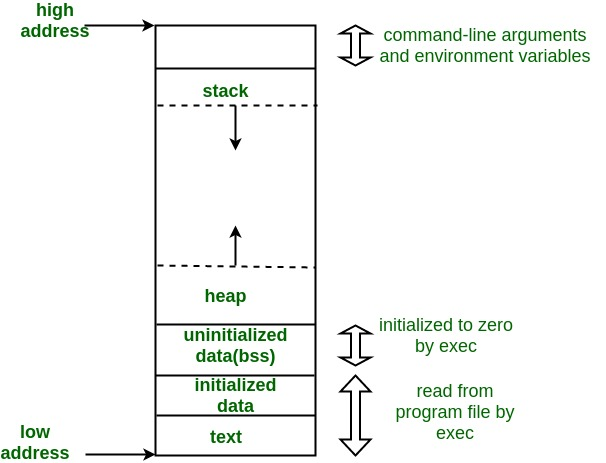
\includegraphics[totalheight=8cm]{images/Cmemory/memoryLayoutC.jpg}
	\begin{minipage}{.6\textwidth}
		%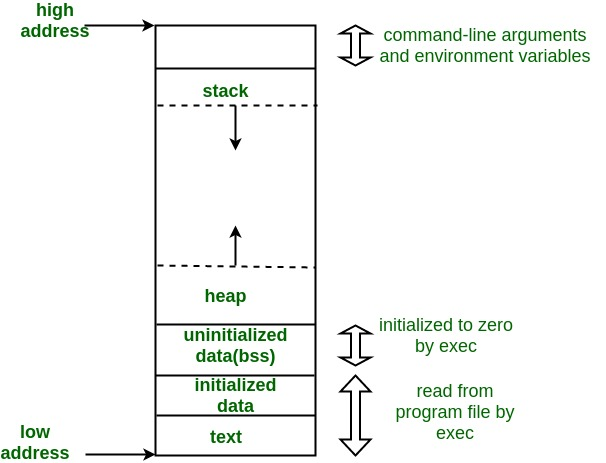
\includegraphics[width=0.4\textwidth]{images/Cmemory/memoryLayoutC.jpg}
		%\caption{cf. \url{https://www.geeksforgeeks.org/memory-layout-of-c-program/}}
		\label{Fig:TypicalCMemoryLayout}
	\end{minipage}



\subsubsection{Mathematical description of strategy for stack buffer overflow exploitation}

Let $n_{\text{stack}} = n_{\text{stack}}(t)$.  Index the stack with $i_{\text{stack}}$ (from "bottom" of the stack to the "top" of the stack):
\[
0 < i_{\text{stack}} < n_{\text{stack}} - 1
\]
Recall that $i_{\text{stack}} \in \mathbb{Z}^+$ and 
\[
i_{\text{stack}} \mapsto \text{high address } - i_{\text{stack}} \equiv x = x(i_{\text{stack}}) \in \text{Addresses}_{\text{Memory block}} \subset \text{Obj}(\textbf{Address})
\]
Let an array of length $L$ (e.g. \verb|char| array) \verb|buf|, with \verb|\&buf| $=$ \verb|\&buf(0)| $\in  \text{Obj}{(\textbf{Address})}$, be s.t. \verb|&buf| $=x(n_{\text{stack}}-1)$ (starts at "top of the stack and "lowest" address of stack at time $t$, s.t. 
\[
\verb|&buf|(j) = \verb|&buf|(0) + j \verb|sizeof|(T)
\]
with $T\in \textbf{Types}$).  


Suppose return address of a function (such as \verb|main|), $\text{eval}(\verb|RIP|)$ be 
\[
\text{eval}(\verb|RIP|) = \verb|&buf| + L \text{or at least } \text{eval}(\verb|RIP|) \geq \verb|&buf| + L
\]
If we write to \verb|buf| more values than $L$, we can write over \text{eval}(\verb|RIP|), making \text{eval}(\verb|RIP|) a different value than before.  




\subsection{Stack}

cf. \url{https://www.geeksforgeeks.org/memory-layout-of-c-program/}

Traditionally, stack area adjoined heap area and they grow in opposite direction. \\
When stack ptr meets heap ptr, free memory exhausted. \\
(with modern large address spaces, virtual memory techniques, they may be placed almost anywhere, but they still typically grow opposite direction)  \\

stack area contains program stack, UFO structure, typically located in higher parts of memory. \\
On standard x86, grows toward address 0. \\
"stack ptr" register tracks top of stack, adjusted to point to top each time a value is "pushed" onto stack. \\
set of values pushed for 1 function call is "stack frame", stack frame consists at minimum of return address. 

Newly called function allocates room on stack for its automatic and temporary variables. \\
$\Longrightarrow$ recursion: each time recursive function calls itself, new stack frame is used, so 1 set of variables (in recursion) doesn't interfere with variables from another instance of the function. 

cf. \href{https://www.tutorialspoint.com/where-are-static-variables-stored-in-c-cplusplus}{Where are static variables in C/C++? Tutorialspoint}

static variables remain in memory; lifetime is entire program, stored in data segment of memory (near heap); data segment is part of virtual address space of a program.

asked here \url{https://www.codingame.com/work/cpp-interview-questions/}, what is a static variable


cf. Ferres (2010) \cite{Ferr2010}

Stack and functions: When a function executes, it may add some of its state data to top of the stack (EY : 20171111, stack grows downward, so "top" is smallest address?); when function exits, stack is responsible for removing that data from stack.  

In most modern computer systems, each thread has a reserved region of memory, stack.  Thread's stack is used to store location of function calls in order to allow return statements to return to the correct location.  

\begin{itemize}
	\item OS allocates stack for each system-level thread when thread is created.  
	\item Stack is attached to thread, so when thread exits, that stack is reclaimed, vs. heap typically allocated by application at runtime, and is reclaimed when application exits.  
	\item When thread is created, stack size is set.  
	\item Each byte in stack tends to be reused frequently, meaning it tends to be mapped to the processor's cache, making if very fast.  
	\item Stored in computer RAM, \emph{just like} the heap.  
	\item Implemented with an actual stack data structure.  
	\item stores local data, return addresses, used for parameter passing  
	\item Stack overflow, when too much stack is used (mostly from infinite (or too much) recursion, and very large allocation)
	\item Data created on stack can be used without pointers.  
\end{itemize}

Also note, for \textbf{physical location in memory}, because of \href{http://en.wikipedia.org/wiki/Virtual_memory}{Virtual Memory}, makes your program think that you have access to certain addresses where physical data is somewhere else (even on hard disc!).  Addresses you get for stack are in increasing order as your call tree gets deeper.  

\href{http://stackoverflow.com/questions/79923/what-and-where-are-the-stack-and-heap/79988#79988}{memory management - What and where are the stack and heap? Stack Overflow, Tom Leys' answer}

cf. \url{https://stackoverflow.com/questions/79923/what-and-where-are-the-stack-and-heap/80113#80113}  

Stack is memory set aside for a thread of execution.  Each thread gets a stack, while there's typically only 1 heap for the application (although it isn't uncommon to have multiple heaps for different types of allocation).  

"
\begin{quotation}
To what extent are they controlled by the OS or language runtime?
\end{quotation}

The OS allocates the stack for each system-level thread when the thread is created. Typically the OS is called by the language runtime to allocate the heap for the application.

\begin{quotation}
What is their scope?
\end{quotation}

\begin{quotation}
The stack is attached to a thread, so when the thread exits the stack is reclaimed. The heap is typically allocated at application startup by the runtime, and is reclaimed when the application (technically process) exits.
\end{quotation}

\begin{quotation}
What determines the size of each of them?
\end{quotation}

The size of the stack is set when a thread is created. The size of the heap is set on application startup, but can grow as space is needed (the allocator requests more memory from the operating system).




\subsection{Stack overflow}  

If you use heap memory, and you overstep the bounds of your allocated block, you have a decent chance of triggering a segmentation fault (not 100%, since your block may be incidentally contiguous with another that you have previously allocated), says Ferres (2010) \cite{Ferr2010}.  

On stack, since variables created on stack are always contiguous with each other; writing out of bounds can change the value of another variable.  e.g. buffer overflow.  

\subsection{Heap}  

Heap contains a linked list of used and free blocks.  New allocations on the heap (by \verb|new| or \verb|malloc|) are satisfied by creating suitable blocks from free blocks.  

This requires updating list of blocks on the heap.  This meta information about the blocks on the heap is stored \emph{on the heap} often in a small area in front of every block.  

\begin{itemize}
	\item Heap size set on application startup, but can grow as space is needed (allocator requests more memory from OS)
	\item heap, stored in computer RAM, like stack.
\end{itemize}

\subsubsection{Memory leaks}  

Memory leaks occurs when computer program consumes memory, but memory isn't released back to operating system.  

"Typically, a memory leak occurs because dynamically allocated memory becomes unreachable."  (Ferres (2010) \cite{Ferr2010}).  

Programs \verb|./Cmemory/heapstack/Memleak.c| deliberately leaks memory by losing the pointer to allocated memory.  

Note, generally, the OS delays real memory allocation until something is written into it, so program ends when virtual addresses run out of bounds (per process limits).  

\subsection{Segmentation Fault}

\url{https://en.wikipedia.org/wiki/Segmentation_fault}

Failure condition (i.e. fault) that software attempted to access restricted area of memory (memory access violation).

"Segmentation" in this context refers to address space of a \emph{program}.



\subsection{More Segmentation Faults}  

The operating system (OS) is running the program (its instructions).  Only from the hardware, with \href{https://en.wikipedia.org/wiki/Memory_protection}{memory protection}, with the OS be signaled to a memory access violation, such as writing to read-only memory or writing outside of allotted-to-the-program memory, i.e. data segments.  On \verb|x86_64| computers, this \href{https://en.wikipedia.org/wiki/General_protection_fault}{general protection fault} is initiated by protection mechanisms from the hardware (processor).  From there, OS can signal the fault to the (running) process, and stop it (abnormal termination) and sometimes core dump. 

For \href{https://en.wikipedia.org/wiki/Virtual_memory}{virtual memory}, the memory addresses are mapped by program called \emph{virtual addresses} into \emph{physical addresses} and the OS manages virtual addresses space, hardcare in the CPU called memory management unit (\emph{MMU}) translates virtual addresses to physical addresses, and kernel manages memory hierarchy (eliminating possible overlays).  In this case, it's the \emph{hardware} that detects an attempt to refer to a non-existent segment, or location outside the bounds of a segment, or to refer to location not allowed by permissions for that segment (e.g. write on read-only memory).          

\subsubsection{Dereferencing a ptr to a NULL ptr (in C) at OS, hardware level}

  
The problem, whether it's for dereferencing a pointer that is a null pointer, or uninitialized pointer, appears to (see the \verb|./Cmemory/| subfolder) be at this instruction at the register level:  

\begin{lstlisting}
x000000000040056c <+38>:	movzbl (%rax),%eax

// or 

0x00000000004004be <+24>:	movss  %xmm0,(%rax)  
\end{lstlisting}

involving the register RAX, a temporary register and to return a value, upon assignment.  And in either case, register RAX has trying to access virtual (memory) address \verb|0x0| (to find this out in \verb|gdb|, do \verb|i r| or \verb|info register|).  

Modern OS's run user-level code in a mode, such as \emph{protected mode}, that uses "paging" (using secondary memory source than main memory) to convert virtual addresses into physical addresses.  

For each process (thread?), the OS keeps a \emph{page table} dictating how addresses are mapped.  Page table is stored in memory (and protected, so user-level code can't modify it).  For every memory access, given (memory) address, CPU translates address according to the page table.  

When address translation fails, as in the case that \emph{not all addresses are valid}, and so if a memory access generates an invalid address, the processor (hardware!) raises a \emph{page fault exception}.  "This triggers a transition from \emph{user mode} (aka \emph{current privilege level (CPL) 3} on x86/x86-64) into \emph{kernel mode} (aka CPL 0) to a specific location in the kernel's code, as defined by the \emph{interrupt descriptor table} (IDT)."  cf. \href{https://stackoverflow.com/questions/12645647/what-happens-in-os-when-we-dereference-a-null-pointer-in-c}{What happens in OS when we dereference a NULL pointer in C?}


Kernel regains control and send signal (EY : 20171115 to the OS, I believe).   

In modern OS's, page tables are usually set up to make the address 0 an invalid virtual address.  

cf. \href{https://stackoverflow.com/questions/12645647/what-happens-in-os-when-we-dereference-a-null-pointer-in-c}{What happens in OS when we dereference a NULL pointer in C?}

\subsubsection{Page Faults aren't "faults"}

\url{https://scoutapm.com/blog/understanding-page-faults-and-memory-swap-in-outs-when-should-you-worry}

Linux allocates memory to processes by dividing physical memory into pages, and then mapping those physical pages to virtual memory needed by a process. It does this in conjunction with the Memory Management Unit (MMU) in the CPU.
\begin{itemize}
	\item Typically a page will represent 4KB of physical memory.
	\item Statistics and flags are kept about each page to tell Linux the status of that chunk of memory.
	\item These pages can be in different states; some free (unused), some used to hold executable code, some allocated as data for a program.
\end{itemize}

For example, consider a large running program on a Linux system.

\begin{itemize}
	\item Program executable size could be measured in megabytes, but not all that code will run at once.
	\begin{itemize}
		\item Some of the code will only be run during initialization or when a special condition occurs
		\item Over time, Linux can discard pages of memory which hold executable code, if it thinks they're no longer needed or will be used rarely.
	\end{itemize}
\end{itemize}

A program is executed by CPU as it steps its way through the machine code.
\begin{itemize}
	\item Each instruction is stored in physical memory at a certain address.
\end{itemize}

\part{C++}  

\section{Pass by reference, pass by value, pointers vs. reference}

In C++, pass arguments into a function in these different ways:
\begin{itemize}
	\item Call by Value
	\item Call by Reference
	\item Call by Address
\end{itemize}
cf. \href{https://www.tutorialspoint.com/differences-between-pass-by-value-and-pass-by-reference-in-cplusplus}{Differences between pass by value and pass by reference in C++, Tutorialspoint}

Call by address, use pointer variables to send exact memory address, but call by reference, pass reference variable (alias of that variable).

\subsection{Call by Value}

Actual value that's passed as arguments isn't changed after performing some operation on it. When call by value used, it creates a copy of that variable into stack section in memory. When value changed, it changes value of that copy, the actual value remains the same.

cf. \href{https://www.cs.fsu.edu/~myers/c++/notes/references.html}{FSU, Myers}

Any r-values may be sent in.

Local parameters are copies of original arguments passed in.

Changes made in function to these variables don't affect originals.

\subsection{Call by Reference}

When call by reference is used, it creates a copy of the reference of that variable into stack section in memory. When value is changed using the reference it changes value of the actual variable.

Use call by reference mainly when we want to change value of passed argument into invoker function.\\
Also, since 1 function can return only 1 value, when we need more than 1 value from a function, we pass them as an output argument in this manner.

When function expects strict reference types in parameter list, an L-value (i.e. variable, or storage location) must be passed in.

Local parameters are references to storage locations of original arguments passed in.

Changes to these variables in function will affect originals.

\emph{No copy is made}, so overhead of copying (time, storage) is saved.

cf. \href{https://www.cs.fsu.edu/~myers/c++/notes/references.html}{FSU, Myers}


\section{static}



\section{Free Store}  


cf. \href{http://www.gotw.ca/gotw/009.htm}{GotW \#9, Memory Management - Part I}

Free store is 1 of the 2 dynamic memory areas, allocated/freed by new/delete (free store and heap).  Object lifetime can be less than the time the storage is allocated.  

Let $t_{0,\text{obj}}, t_{f,\text{obj}}$, $t_{f,\text{obj}} \geq t_{0,\text{obj}}$, \\
\phantom{Let } $t_{0,\text{alloc}}, t_{f,\text{alloc}}$, $t_{f,\text{alloc}} \geq t_{0,\text{alloc}}$, \\  
with the condition that 
\[
t_{0,\text{alloc}} \leq t_{0,\text{obj}} \leq t_{f,\text{obj}} \leq t_{f,\text{alloc}}
\].  

For $t \in (t_{0,\text{alloc}} , t_{0,\text{obj}} )$, storage may be accessed and manipulated through a \verb|void*| but non of the proto-object's \emph{nonstatic} members or member functions may be accessed, have their addresses taken, or be otherwise manipulated.  




cf. 11.2 Introduction of Ch. 11 Select Operations \cite{Stro2013}.  




\section{Copy vs. Move}  
cf. 17.1 Introduction of Ch. 17 Construction, Cleanup, Copy, and Move of Stroustrup \cite{Stro2013}.  

Gottschling (2015) \cite{Gott2015}

\subsection{Constructors and Invariants}

cf. 17.2.1 Constructors and Invariants, pp. 484, Ch. 17, Stroustrup \cite{Stro2013}.

\textbf{class invariant} - something that must hold whenever a member function is called (from outside the class). Typically, class \emph{constructor}'s job is to initialize an object of its class and that initialization must establish the \emph{class invariant}.

For example
\begin{lstlisting}
Vector::Vector(int s)
{
  if (s<0) throw Bad_size{s};
  sz = s;
  elem = new double[s];
}
\end{lstlisting}

Constructor must make true that an array size must be non-negative.

Why would you define an invariant?
\begin{itemize}
	\item To focus the design effort for the class
	\item To clarify behavior of the class (e.g., under error conditions)
	\item To simplify definition of member functions
	\item To clarify class's management of resources
	\item To simplify documentation of the class
\end{itemize}

\subsection{Base and Member Destructors}

cf. 17.2.3 Base and Member Destructors, pp. 486, Stroustrup \cite{Stro2013}.

Ctors and dtors interact correctly with class hierarchies. A constructor builds a class object "from the bottom up":
\begin{enumerate}
	\item first, ctor invokes its base class constructors
	\item then, it invokes the member constructors, and
	\item finally, it executes its own body
\end{enumerate}
A dtor "tears down" an object in reverse order:
\begin{enumerate}
	\item first, dtor executes its own body,
	\item then, it invokes its member dtors, and
	\item finally, it invokes its base class dtors
\end{enumerate}

In particular, a \verb|virtual| base is constructed before any base that might use it and destroyed after all such bases - this ordering ensures that a base or member isn't used before it has been initialized or used after it has been destroyed.

\subsection{virtual Destructors}

A dtor can be declared to be \verb|virtual|, and usually should be for a class with a virtual function. The reason we need a \verb|virtual| dtor is that an object usually manipulated through the interface provided by a base class is often also \verb|delete|'d through that interface. It's because a derived class would have its own dtor, and without \verb|virtual|, \verb|delete| would fail to invoke appropriate derived class dtor.

\begin{lstlisting}
class Shape
{
  public:
    virtual void draw() = 0;
    virtual ~Shape();
};

class Circle
{
  public:
	void draw();
	~Circle(); // overrides ~Shape()
};

void user(Shape* p)
{
  p->draw(); // invoke appropriate draw()
  delete p; // invoke appropriate dtor
}
\end{lstlisting}


Difference between \emph{move} and \emph{copy}: after a copy, 2 objects must have same value; whereas after a move, the source of the move isn't required to have its original value.  So moves can be used when source object won't be used again.  

Refs.: Sec. 3.2.1.2, Sec. 5.2, notion of moving a resource, Sec. 13.2-Sec.13.3, object lifetime and errors explored further in Stroustrup \cite{Stro2013}  
  
  
5 situations in which an object is copied or moved:   
\begin{itemize}
	\item as source of an \emph{assignment}
	\item as object initializer 
	\item as function argument
	\item as function return value
	\item as an exception  
\end{itemize}


\subsection{Copy constructor}

cf. \href{http://en.cppreference.com/w/cpp/language/copy_constructor}{Copy constructors, cppreference.com}

Copy constructor of class T is non-template constructor whose 1st parameter is \verb|T&, const T&, volatile T&|, or \verb|const volatile T&|.  

\subsubsection{Syntax}  

\begin{lstlisting}
class_name ( const class_name & )  
class_name ( const class_name & ) = default;  
class_name ( const class_name & ) = delete;
\end{lstlisting}  

\subsubsection{Explanation}  
\begin{enumerate}
\item Typical declaration of a copy constructor.  
\item Forcing copy constructor to be generated by the compiler.  
\item Avoiding implicit generation of copy constructor.  
\end{enumerate}


Copy constructor called whenever an object is \textbf{initialized} (by \textbf{direct-initialization} or \textbf{copy-initialization}) from another object of same type (unless \textbf{overload resolution} selects better match or call is \textbf{elided} (???)), which includes  
\begin{itemize}
\item initialization \verb|T a = b;| or \verb|T a(b);|, where b is of type T;  
\item function argument passing: \verb|f(a);|, where a is of type T and f is \verb|void f(T t)|;  
\item function return: \verb|return a;| inside function such as \verb|T f()|, where a is of type T, which has no \textbf{move constructor}.   
\end{itemize}

\subsubsection{Example}  

\begin{lstlisting}
struct A
{
	int n;
	A(int n = 1) : n(n) { }
	A(const A& a) : n(a.n) { } // user-defined copy ctor
};

struct B : A
{
	// implicit default ctor B::B()
	// implicit copy ctor B::B(const B&)
};

int main()
{
	A a1(7);
	A a2(a1); // calls the copy ctor
	B b;
	B b2 = b;
	A a3 = b; // conversion to A& and copy ctor  
}
\end{lstlisting}  

i.e. cf. \href{http://www.geeksforgeeks.org/copy-constructor-in-cpp/}{Copy Constructor in C++}

\begin{definition}
	\textbf{Copy constructor} is a member function which initializes an object using another object of the same class.  
\end{definition}

\subsubsection{When is copy constructor called? } 
\begin{enumerate}
\item When object of class returned by value 
\item When object of class is passed (to a function) by value as an \textbf{argument}.  
\item When object is constructed based on another object of same class  (or overloaded)  
\item When compiler generates temporary object  
\end{enumerate}


However, it's not guaranteed copy constructor will be called in all cases, because C++ standard allows compiler to optimize the copy away in certain cases.  

\subsubsection{When is used defined copy constructor needed?  shallow copy, deep copy}  

If we don't define our own copy constructor, C++ compiler creates default copy constructor which does member-wise copy between objects.  

We need to define our own copy constructor only if an object has pointers or any run-time allocation of resource like file handle, network connection, etc.  

\subsubsection{Default constructor does only shallow copy.}  

\subsubsection{Deep copy is possible only with user-defined copy constructor.}  

We thus make sure pointers (or references) of copied object point to new memory locations.  

\subsubsection{Copy constructor vs. Assignment Operator}  

\begin{lstlisting}  
MyClass t1, t2; 
MyClass t3 = t1; 	// ----> (1)
t2 = t1; 			// -----> (2)
\end{lstlisting}

Copy constructor called when new object created from an existing object, as copy of existing object, in (1).  
Assignment operator called when already initialized object is assigned a new value from another existing object, as assignment operator is called in (2).  

\subsubsection{Why argument to a copy constructor should be const?  } 

cf. \href{http://www.geeksforgeeks.org/copy-constructor-argument-const/}{Why copy constructor argument should be const in C++?, geeksforgeeks.org}

\begin{enumerate}
\item Use \verb|const| in C++ whenever possible so objects aren't accidentally modified.  
\item e.g.  
\end{enumerate}

\begin{lstlisting}  
#include <iostream>  

class Test
{
	/* Class data members */
	public:
	Test(Test &t) 	{ /* Copy data members from t */ } 
	Test()			{ /* Initialize data members */ }
};

Test fun() 
{
	Test t;
	return t;
};

int main()
{
	Test t1;
	Test t2 = fun();  error: invalid initialization of non-const reference of type Test& from an rvalue of type Test
}
\end{lstlisting}

\verb|fun()| returns by value, so compiler creates temporary object which is copied to t2 using copy constructor (because this temporary object is passed as argument to copy constructor since compiler generates temp. object).  
Compiler error is because \textbf{compiler-created temporary objects cannot be bound to non-const references}. 



\subsection{Move Constructor}  

For a class, to control what happens when we move, or move and assign object of this class type, use special member function \emph{move constructor}, \emph{move-assignment operator}, and define these operations.  Move constructor and move-assignment operator take a (usually nonconst) rvalue reference, to its type.  Typically, move constructor moves data from its parameter into the newly created object.  After move, it must be safe to run the destructor on the given argument.  cf. Ch. 13 of Lippman, Lajole, and Moo (2012) \cite{LLM2012}



\section{vtable; virtual table}  

I was given this answer to a question I posed to a 20 year C++ veteran and it was such an important answer (as I did not know a virtual table existed, at all before), that I will copy this, repeat this and explore this extensively:  

"The keyword you're looking for is virtual table: " \href{https://stackoverflow.com/questions/99297/how-are-virtual-functions-and-vtable-implemented}{How are virtual functions and vtable implemented?, stackoverflow}  

Original question, from \href{https://stackoverflow.com/users/3153/brian-r-bondy}{Brian R. Bondy}:  

\subsection{How are virtual functions and vtable implemented?}

We all know what virtual functions are in C++, but how are they implemented at a deep level?

Can the vtable be modified or even directly accessed at runtime?

Does the vtable exist for all classes, or only those that have at least one virtual function?

Do abstract classes simply have a NULL for the function pointer of at least one entry?

Does having a single virtual function slow down the whole class? Or only the call to the function that is virtual? And does the speed get affected if the virtual function is actually overwritten or not, or does this have no effect so long as it is virtual.

Answer from \emph{community wiki}:  

\subsubsection{How are virtual functions implemented at a deep level?}

From \href{http://wayback.archive.org/web/20100209040010/http://www.codersource.net/published/view/325/virtual_functions_in.aspx}{"Virtual Functions in C++"}

Whenever a program has a virtual function declared, a v - table is constructed for the class. The v-table consists of addresses to the virtual functions for classes that contain one or more virtual functions. The object of the class containing the virtual function contains a virtual pointer that points to the base address of the virtual table in memory.  

Whenever there is a virtual function call, the v-table is used to resolve to the function address.  

An object of the class that contains one or more virtual functions contains a virtual pointer called the vptr at the very beginning of the object in the memory. Hence the size of the object in this case increases by the size of the pointer. This vptr contains the base address of the virtual table in memory.  

Note that virtual tables are class specific, i.e., there is only one virtual table for a class irrespective of the number of virtual functions it contains. This virtual table in turn contains the base addresses of one or more virtual functions of the class. At the time when a virtual function is called on an object, the vptr of that object provides the base address of the virtual table for that class in memory. This table is used to resolve the function call as it contains the addresses of all the virtual functions of that class. This is how dynamic binding is resolved during a virtual function call.

cf. \href{http://wayback.archive.org/web/20100209040010/http://www.codersource.net/published/view/325/virtual_functions_in.aspx}{"Virtual Functions in C++"}

\subsubsection{What is a Virtual Function?}  

A virtual function is a member function of a class, whose functionality can be over-ridden in its derived classes. It is one that is declared as virtual in the base class using the virtual keyword. The virtual nature is inherited in the subsequent derived classes and the virtual keyword need not be re-stated there. The whole function body can be replaced with a new set of implementation in the derived class. 

\subsubsection{What is Binding?}  

Binding is associating an object or a class with its member.   If we call a method \verb|fn()| on an object \verb|o| of a class \verb|c|, we say that object \verb|o| is binded with method \verb|fn()|.  

This happens at \emph{compile time} and is known as \emph{static} - or \emph{compile-time} binding.   

Calls to virtual member functions are resolved during \emph{run-time}.  This mechanisms is known as \emph{dynamic-binding.}   

The most prominent reason why a virtual function will be used is to have a different functionality in the derived class.  The difference between a non-virtual member function and a virtual member function is, the non-virtual member functions are resolved at compile time.  

\subsubsection{How does a Virtual Function work?}  

When a program (code text?) has a virtual function declared, a \textbf{v-table} is \emph{constructed} for the class.  

The v-table consists of addresses to virtual functions for classes that contain 1 or more virtual functions.  \\
The object of the class containing the virtual function \emph{contains a virtual pointer} that points to the base address of the virtual table in memory.  An object of the class that contains 1 or more virtual functions contains a virtual pointer called the \textbf{vptr} at the very beginning of the object in the memory.  (Hence size of the object in this case increases by the size of the pointer; "memory/size overhead.")  \\

This vptr is added as a hidden member of this object.  As such, compiler must generate "hidden" code in the \textbf{constructors} of each class to initialize a new object's vptr to the address of its class's vtable.  

Whenever there's a virtual function call, vtable is used to resolve to the function address.  
This vptr contains base address of the virtual table in memory.  \\

Note that virtual tables are class specific, i.e. there's only 1 virtual table for a class, irrespective of number of virtual functions it contains, i.e.  

vtable is same for all objects belonging to the same class, and typically is shared between them.    
  

This virtual table in turn contains base addresses of 1 or more virtual functions of the class.  

At the time when a virtual function is called on an object, the vptr of that object provides the base address of the virtual table for that class in memory.  This table is used to resolve the function call as it contains the addresses of all the virtual functions of that class.  This is how dynamic binding is resolved during a virtual function call, i.e.  

class (inherited or base/parent) cannot, generally, be determined \emph{statically} (i.e. \textbf{compile-time}), so compiler can't decide which function to call at that (compile) time.  (Virtual function) call must be dispatched to the right function \emph{dynamically} (i.e. \textbf{run-time}).  

  

\subsubsection{Virtual Constructors and Destructors}  

A constructor cannot be virtual because at the time when constructor is invoked, the vtable wouldn't be available in memory.  Hence, we can't have a virtual constructor.  

A virtual destructor is 1 that's declared as virtual in the base class, and is used to ensure that destructors are called in the proper order.  Remember that destructors are called in reverse order of inheritance.  If a base class pointer points to a derived class object, and we some time later use the delete operator to delete the object, then the derived class destructor is not called.  

Finally, the article \href{http://wayback.archive.org/web/20100209040010/http://www.codersource.net/published/view/325/virtual_functions_in.aspx}{"Virtual Functions in C++"} concludes, saying, "Virtual methods should be used judiciously as they are slow due to the overhead involved in searching the virtual table. They also increase the size of an object of a class by the size of a pointer. The size of a pointer depends on the size of an integer."  I will have to check this with other references, because, first of all, how then would class inheritance be otherwise implemented?  

cf. \href{https://stackoverflow.com/questions/99297/how-are-virtual-functions-and-vtable-implemented}{How are virtual functions and vtable implemented?, stackoverflow}  

\subsubsection{Can the vtable be modified or even directly accessed at runtime?  No.}  

"Universally, I believe the answer is "no". You could do some memory mangling to find the vtable but you still wouldn't know what the function signature looks like to call it. Anything that you would want to achieve with this ability (that the language supports) should be possible without access to the vtable directly or modifying it at runtime. Also note, the C++ language spec does not specify that vtables are required - however that is how most compilers implement virtual functions."  

\subsubsection{Do abstract classes simply have a NULL for the function pointer of at least one entry?  Some do place NULL pointer in vtable, some place pointer to dummy method; in general, undefined behavior}

The answer is it is unspecified by the language spec so it depends on the implementation. Calling the pure virtual function results in undefined behavior if it is not defined (which it usually isn't) (ISO/IEC 14882:2003 10.4-2). In practice it does allocate a slot in the vtable for the function but does not assign an address to it. This leaves the vtable incomplete which requires the derived classes to implement the function and complete the vtable. Some implementations do simply place a NULL pointer in the vtable entry; other implementations place a pointer to a dummy method that does something similar to an assertion.

Note that an abstract class can define an implementation for a pure virtual function, but that function can only be called with a qualified-id syntax (ie., fully specifying the class in the method name, similar to calling a base class method from a derived class). This is done to provide an easy to use default implementation, while still requiring that a derived class provide an override.

\subsection{pImpl, shallow copy, deep copy}  

cf. Item 22: "When using the Pimpl Idiom, define special member functions in the implementation file," pp. 147 of Meyers (2014) \cite{ScMe2014}.  

\begin{lstlisting}
class Widget { 			// still in header "widget.h" 
	public:
		Widget();
		~Widget();		// dtor is needed-see below 
		... 
	
	private:
		struct Impl;	// declare implementation struct 
		Impl *pImpl;	// and pointer to it
};
\end{lstlisting}

Because \verb|Widget| no longer mentions types \verb|std::string, std::vector|, and \verb|Gadget, Widget| clients no longer need to \verb|\#include| headers for these types.  That speeds compilation.  

\emph{incomplete type} is a type that has been declared, but not defined, e.g. \verb|Widget::Impl|.  There are very few things you can do with an incomplete type, but declaring a pointer to it is 1 of them.  

\verb|std::unique_ptr|s is advertised as supporting incomplete types.  But, when \verb|Widget w;|, \verb|w|, is destroyed (e.g. goes out of scope), destructor is called and if in class definition using \verb|std::unique_ptr|, we didn't declare destructor, compiler generates destructor, and so compiler inserts code to call destructor for \verb|Widget|'s data member \verb|m_Impl| (or \verb|pImpl|).  

\verb|m_Impl| (or \verb|pImpl|) is a \verb|std::unique_ptr<Widget::Impl>|, i.e., a \verb|std::unique_ptr| using default deleter. The default deleter is a function that uses \verb|delete| on raw pointer inside the \verb|std::unique_ptr|.  Prior to using \verb|delete|, however, implementations typically have default deleter employ C++11's \verb|static_assert| to ensure that raw pointer doesn't point to an incomplete type.  When compiler generates code for the destruction of the \verb|Widget w|, then, it generally encounters a \verb|static_assert| that fails, and that's usually what leads to the error message.  

To fix the problem, you need to make sure that at point where code to destroy \verb|std::unique_ptr<Widget::Impl>| is generated, \verb|Widget::Impl| is a complete type.  The type becomes complete when its definition has been seen, and \verb|Widget::Impl| is defined inside \verb|widget.cpp|.  For successful compilation, have compiler see body of \verb|Widget|'s destructor (i.e. place where compiler will generate code to destroy the \verb|std::unique_ptr| data member) only inside \verb|widget.cpp| after \verb|Widget::Impl| has been defined.  

For compiler-generated move assignment operator, move assignment operator needs to destroy object pointed to by \verb|m_Impl| (or \verb|pImpl|) before reassigning it, but in the \verb|Widget| header file, \verb|m_Impl| (or \verb|pImpl|) points to an incomplete type.  Situation is different for move constructor.  Problem there is that compilers typically generate code to destroy \verb|pImpl| in the event that an exception arises inside the move constructor, and destroying \verb|pImpl| requires \verb|Impl| be complete.  

Because problem is same as before, so is the fix - \emph{move definition of move operations into the implementation file}.  

For copying data members, support copy operations by writing these functions ourselves, because (1) compilers won't generate copy operations for classes with move-only types like \verb|std::unique_ptr| and (2) even if they did, generated functions would copy only the \verb|std::unique_ptr| (i.e. perform a \emph{shallow copy}), and we want to copy what the pointer points to (i.e., perform a \emph{deep copy}).  

If we use \verb|std::shared_ptr|, there'd be no need to declare destructor in \verb|Widget|.  

Difference stems from differing ways smart pointers support custom deleters.  For \verb|std::unique_ptr|, type of deleter is part of type of smart pointer, and this makes it possible for compilers to generate smaller runtime data structures and faster runtime code.  A consequence of this greater efficiency is that pointed-to types must be complete when compiler-generated special functions (e.g. destructors or move operations) are used.  For \verb|std::shared_ptr|, type of deleter is not part of the type of smart pointer.  This necessitates larger runtime data structures and somewhat slower code, but pointed-to types need not be complete when compiler-generated special functions are employed.  

\section{Class Hierarchies}

\subsection{Inheritance}

Ctors of inherited classes are called in same order in which they're inherited. Dtors are called in reverse order of ctors.

\subsubsection{Diamond Problem}

cf. \href{https://www.geeksforgeeks.org/multiple-inheritance-in-c/}{Geeks for Geeks, "Multiple Inheritance in C++"}.

Diamond problem occurs when 2 superclasses of a class have a common base class. The class gets 2 copies of all attributes of common base class, causing ambiguities.

\section{Polymorphism}

\textbf{Polymorphism, TODO}

cf. Vandevoorde, Josuttis, and Gregor (2017) \cite{VJG2017}, Ch. 22, pp. 517

Ch. 18 had described static polymorphism (templates), and dynamic polymorphism (inheritance, virtual functions). Tradeoffs: static polymorphism provides same performance as nonpolymorphic code, but set of types that can be used at run time is fixed at compile time. Dynamic polymorphism via inheritance allows a single version of the polymorphic function to work with types not known at time it's compiled, but it's less flexible because types must inherit from a common base class.

Ch. 22 - how to have smaller executable code size and (almost) entirely compiled nature of dynamic polymorphism, along with interface flexibility of static polymorphism that allows, for example, built-in types to work seemlessly.

Gutman (2016) \cite{Gutt2016}

\subsection{Operator Overloading}

cf. 18.2.4 "Passing Objects", pp. 532-533 of Stroustrup (2013) \cite{Stro2013}

For arguments, we have 2 main choices for passing in objects to an operator: 
\begin{itemize}
\item Pass-by-value
\item Pass-by-reference
\end{itemize}

Typically, an operator returns a result. Returning a pointer or reference to a newly created object is usually a bad idea: using a pointer gives notational problems, and referring to an object on free store (whether by pointer or by reference) results in memory management problems. INstead, return objects by value. For large objects, define move operations to make such transfers of values (i.e. return by value) efficient.

If a function simply passes an object to another function, an rvalue reference argument  should be used.

cf. 2.7.3 "Member or Free Function", Gottschling (2015) \cite{Gott2015}

Writing all 3 implementations (binary operator adding two complex class instances, operator oveload accepting a double as second argument, etc.) provides better performance.

Adding 2 complex class values is more naturally expressed as a free function. To avoid ambiguity, we have to remove the member function with the complex argument.

Subtle difference: free functions are selected by overload resolution with potential implicit conversion on both arguments while methods are subject to overriding and name hiding when classes are derived.

\textbf{Binary Operators}: Prefer implementing binary operators as free functions.




\section{Exception Handling, Error Handling, Exception Policy}

cf. MIT OCW 6.005 Software Construction, Spring 2016.

\subsection{Handling Exception Results with Special Values Shall Be Discouraged}

Nearly all the Linux system calls I have encountered are designed like this: you get a return value of -1 to indicate an error when you are expecting a non-negative number for nominal operation, or a, for example, \verb|null| reference when expecting an object. 

Special values for indicating error has 2 problems:
\begin{itemize}
	\item Tedious to check the return value; there is a cost to if-else branching.
	\item It's easy to forget to do it (i.e. to do the check); this would leave the original object or data in a bad state possibly.
\end{itemize}
Furthermore, for the user, it's easy to forget which special values indicate what error if there was one, and with C++17 there is exactly one new mechanism designed for the need to provide a return value for a function that may fail, \verb|std::optional|.


Stroustrup (2013) \cite{Stro2013}

\section{Resources}

Hundreds of easy examples.
\url{https://www.tenouk.com/cpluscodesnippet/cplusarraypointermemoryaddress.html}

\part{Integers, numeric encodings, number representation, binary representation, hexidecimal representation}


\subsection{Information storage}

cf. Ch. 2, Representing and Manipulating Information, pp. 31, Bryant and O'Hallaron (2015) \cite{BrOH2016}

A machine-level program views memory as a very large array of bytes, referred to as \emph{virtual memory}. Every byte of memory is identified by a unique number, known as \emph{address}, and set of all possible addresses known as \emph{virtual address space}. 

Actual implementation (Ch.9, Bryant and O'Hallaron (2015) \cite{BrOH2016}) uses combination of dynamic random access memory (DRAM), flash memory, disk storage, special hardware, and operation system software to provide program with what appears to be a monolithic byte array.

Bryant and O'Hallaron (2015) \cite{BrOH2016} covers in subsequent chapters how compiler and run-time system partitions this memory space into more manageable units to store the different \emph{program objects}, i.e. program data, instructions, and control information.

C compiler maintains \emph{type} information.




\section{Introduction: \texttt{int} $\neq \mathbb{Z}$, \texttt{float} $\neq \mathbb{R}$}

cf. \href{https://www.cs.utexas.edu/users/fussell/courses/cs429h/lectures/Lecture_1-429h.pdf}{Systems 1, Introduction to Computer Systems, Introduction lecture at University of Texas, CS429; Don Fussell}.

\texttt{int} $\neq \mathbb{Z}$, \texttt{float} $\neq \mathbb{R}$

e.g. $x^2 \geq 0$? 

\texttt{float}: Yes!  \\
\texttt{int}: $40000 \times 40000 \to 1600000000$ \\
\phantom{int} $50000 \times 50000 \to $ ??

Is $(x+y) + z = x + (y +z)?$

\texttt{unsigned} and \texttt{signed int}: Yes!

\texttt{float}'s 
\[
\begin{gathered}
(1e20 + -1e20) + 3.14 \to 3.14 \\
1e20 + (-1e20 + 3.14) \to ??
\end{gathered}
\]

Can't assume "usual" properties due to finiteness of representations, so that integer operations satisfy "ring" properties
- commutativity, associativity, distributivity

floating point operations satisfy "ordering" properties
- monotonicity, values of signs


\section{Bits and Bytes}

cf. \href{https://www.cs.utexas.edu/users/fussell/courses/cs429h/lectures/Lecture_2-429h.pdf}{Lecture 2, Bits and Bytes, CS429}.

Consider a (number) system with radix or base $b$ ($b>1$), \\
string of digits $d_1, \dots , d_n$, \\
\begin{equation}
c = \sum_{i=1}^n d_i b^{n-i}, \qquad \, 0 \leq d_i < b \qquad \forall \, i = 1 \dots n 
\end{equation}

with notation $c \equiv c_b$ to help denote the base or "radix", e.g. $15213_{10}$, $00000000_2$.

Byte $\equiv B$, 1 Byte $ = 8$ bits. Note that $2^8 = 256$

e.g. Binary $00000000_2$ to $11111111_2$ \\
Decimal: $0_{10}$ to $255_{10}$ \\
Hexadecimal: $00_{16}$ to $FF_{16}$

cf. Sec. 2.1.1. Hexadecimal Notation, pp. 37, Bryant and O'Hallaron (2015) \cite{BrOH2016}

A single byte $B$ consists of 8 bits. \\
$B$ ranges from, in binary notation, $00000000_2$ to $11111111_2$ \\
$B$ ranges from, in decimal integer, $0_{10}$ to $255_{10}$ \\
$B$ ranges from, in hexadecimale, $00_{16}$ to ${FF}_{16}$. 

In C, numeric constants starting with $0x$ or $0X$ are interpreted as hexadecimal. Characters 'A' through 'F' may be written in either upper- or lowercase. Even mixing upper- and lowercase (e.g. $0xFa1D37b$).

Digits can be converted by referring to Table \ref{Table:HexadecimaleNotation}. \emph{One simple trick for doing the conversion in your head is to memorize the decimal equivalents of hex digits A, C, and F}.

\begin{center}
	\label{Table:HexadecimaleNotation}
	\begin{tabular}{ l | r | r | r | r | r | r | r | r | }
		\hline
		Hex digit & 0 & 1 & 2 & 3 & 4 & 5 & 6 & 7 \\
		Decimal value & 0 & 1 & 2 & 3 & 4 & 5 & 6 & 7 \\
		Binary value & 0000 & 0001 & 0010 & 0011 & 0100 & 0101 & 0110 & 0111 \\
		Hex digit 8 & 9 & A & B & C & D & E & F \\
		Decimal value & 8 & 9 & 10 & 11 & 12 & 13 & 14 & 15 \\
		\hline
	\end{tabular}
\end{center}

Hex values B, D, and E can be translated to decimal by computing their values relative to the first 3.

e.g. Given number $0x173A4C$ - convert this to binary format by expanding each hexadecimal digit

\begin{center}
	\begin{tabular}{ l | r | r | r | r | r | r }
		Hexadecimal & 1 & 7 & 3 & A & 4 & C \\
		Binary & 0001 & 0111& 0011 & 1010 & 0100 & 1100 \\
	\end{tabular}
\end{center}

This gives binary representation $000101110011101001001100$

Conversely, given a binary number, you convert it to hexadecimal by first splitting into groups of 4 bits each.

However, if total number of bits isn't a multiple of 4, you should make the \emph{leftmost} group be the one with fewer than 4 bits, effectively padding the number with leading zeros. e.g. $1111001010110110110011$

\begin{center}
	\begin{tabular}{ l | r | r | r | r | r | r }
		Binary & 11 & 1100 & 1010 & 1101 & 1011 & 0011 \\
		Hexadecimal & 3 & C & A & D & B & 3 \\
	\end{tabular}
\end{center}


\subsection{Machine Words}

Machine has "Word size".

Nominal size of integer-valued data, including addresses.

\subsection{Word-oriented Memory Organization}

Addresses specify Byte locations. 

Addresses of successive words differ by 4 (32-bit) or 8 (64-bit).

32-bit words:

Addr = 0000, Addr = 0004

64-bit words:

Addr = 0000, Addr = 0008

\subsection{Byte-ordering: Big-Endian, Little-Endian}

$b = 8$

\begin{equation}
c = \sum_{i=0}^{n-1} d_i 8^{n-1 -i}
\end{equation}

\textbf{Big-Endian}: Least significant byte has highest address.

For address $a$, 
\[
\begin{gathered}
	a \mapsto d_0 \\
	a+1 \mapsto d_1 \\
\vdots \\
a+n-1 \mapsto d_{n-1}
\end{gathered}
\]

\textbf{Little-Endian}: Least significant byte has lowest address
\[
\begin{gathered}
a \mapsto d_{n-1}  \\
a+1 \mapsto d_{n-2} \\
\vdots \\
a+n -1 \mapsto d_0
\end{gathered}
\]

\subsection{Representing Strings}

C Strings

- represented by array of characters, each character encoded in ASCII format 
- string should by null-terminated meaning final character $=0$

\subsection{Machine-Level Code Representation}

Encode program as sequence of Instructions. 

Each simple operation
- arithmetic operation, read or write memory, conditional branch.
- instructions encoded as bytes, 
i.e. programs are byte sequences too!

\subsection{Boolean Algebra}

Boole's Algebraic representation of logic.

And: \\
$A \& B = 1$ when both $A=1$ and $B=1$

Or: \\
$A | B = 1$ when either $A=1$ or $B=1$

Not: \\
${}^{\sim}A= 1$ when $A=0$, \\
${}^{\sim}A= 0$ when $A=1$, \\

Exclusive-Or (Xor)
$A {}^{\wedge} B = 1$ when either $A=1$ or $B=1$, but not both

\begin{center}
	\begin{tabular}{ l | c  c }
		${}^{\wedge}$ & 0 & 1 \\ \hline 
		0 & 0 & 1 \\
		1 & 1 & 0
	\end{tabular}
\end{center}

\subsubsection{Application of Boolean Algebra}

Claude Shannon 1937 MIT Master's Thesis. Encode closed switch as 1, open switch as 0. Connection when $A\& \sim B | \sim A \& B = A \wedge B$

\subsubsection{Integer Algebra}

$\langle \mathbb{Z}, +, *, - , 0 , 1 \rangle$ forms a ring

\subsubsection{Boolean Algebra}

$\langle \lbrace 0, 1 \rbrace , |, \& , \sim, 0, 1 \rangle $ forms a "Boolean algebra"

Or ($|$) is "sum" operation. \\
And ($\&$) is "product" operation. \\
$\sim$ is "complement" operation. \\
$0$ is additive identity. \\
$1$ is multiplicative identity.

cf. \url{https://en.wikipedia.org/wiki/Bitwise_operation}

Bitwise OR may be used to set to 1 selected bits of register. e.g. fourth bit of 0010 may be set by performing bitwise OR with pattern with only 4th bit set.

Bitwise AND is equivalent to multiplying corresponding bits. Thus, if both bits in compared position are 1, bit in resulting binary representation is ($1 \times 1 = 1$); otherwise result is 0 ($1 \times 0 = 0$ and $0 \times 0 = 0$).

Operation may be used to determine whether particular bit is set (1) or clear (0). e.g. given bit pattern 0011 (decimal 3), to determine whether 2nd bit is set, use bitwise AND with bit pattern containing 1 only in 2nd. bit. Because result 0010 is non-zero, we know 2nd. bit in original pattern is set. This is often called \emph{bit masking} (by analogy, use of masking tape covers, or \emph{masks}, portions that are not of interest)

Bitwise AND may be used to clear selected bits (or flags) of a register in which each bit represents an individual Boolean state.
\begin{itemize}
	\item This technique is an efficient way to store a number of Boolean values using as little memory as possible.
	\item Also, easy to check parity (even or odd?) of binary number by checking value of lowest valued bit.
\end{itemize}

Bitwise XOR may be used to invert selected bits in a register (also called toggle or flip). Any bit may be toggled by XORing with 1. e.g. given bit pattern 0010, 2nd and 4th bits may be toggled by bitwise XOR with bit pattern containing 1 in 2nd. and 4th. positions.



Consider Boolean Ring:
\[
\langle \lbrace 0 , 1 \rbrace, \wedge, \&, I, 0 , 1 \rangle \simeq \mathbb{Z}_2 \equiv  \text{ integers} \mod{2} 
\]
where $I$ is identity operation $I(A) = A$, \\
and 
$A\wedge A = 0$ is the additive inverse (existence) property.

\subsubsection{De Morgan's Laws}

\[
\begin{gathered}
A \& B = \sim (\sim A | \sim B) \\
A | B = \sim (\sim A \& \sim B)
\end{gathered}
\]

\subsubsection{Exclusive-Or using Inclusive Or}

\[
\begin{gathered} 
	A \wedge B = (\sim A \& B) | (A \& \sim B) \\
 A \wedge B = (A | B) \& \sim (A \& B)
\end{gathered} 
\]

All properties of Boolean Algebra apply to bit vectors.

\subsection{Representing and Manipulating Sets; bit vectors as sets}

Width $w$ bit vector represents subsets of $\lbrace 0 ,\dots, w-1 \rbrace$, s.t. for $a\in \lbrace 0 ,1 \rbrace^w$, $a_j \in \lbrace 0 , 1 \rbrace$, $\forall \, j = 0,1,\dots w -1$. 

\qquad \\
If $a_j = 1, j \in A$; otherwise, \\
If $a_j =0$, $j \notin A$
\qquad \\

\subsubsection{Operations}

\qquad \\
$\& \to $ intersection \\
$| \to $ union \\
$\wedge \to $ symmetric difference \\
$\sim \to $ complement
\qquad \\

Logic operations in C: $\& \&$, $||$, $!$ 

Shift operations



cf. \href{https://www.cs.utexas.edu/users/fussell/courses/cs429h/lectures/Lecture_3-429h.pdf}{Systems 1, Integers lecture at University of Texas, CS429} is a \textbf{very good lecture}; both \emph{mathematically rigorous} and full of useful, \emph{clear} examples.

\section{Unsigned integers}

Consider $\mathbb{Z}^+_{2^w} \to \mathbb{Z}^+$, where $\mathbb{Z}^+_{2^w}$ represent "unsigned" integers. 
\begin{equation}
\begin{gathered}
\mathbb{Z}^+_{2^w} \to \mathbb{Z}^+ \\ 
(x_0, x_1 , \dots , x_{w-1}) \mapsto \sum_{i=0}^{w-1} x_i \cdot 2^i 
\end{gathered}
\end{equation}

To recap using CS429's notation, for an unsigned integer $x$, \\
$B2U \equiv $ base-2-unsigned \\
\[
B2U(x) = \sum_{i=0}^{w-1} x_i \cdot 2^i 
\]
where $B2U : "\mathbb{Z}^+" \to \mathbb{Z}^+_{2^w}$

So $w$ is the total number of "bits" to represent $x$.


For hexidecimal (-based) numbers, observe this relationship: 
\begin{equation}
2^w = 16^v = 2^{4v} \text{ so } w =4v
\end{equation}

So for a hexidecimal number, $v$ hexidecimal numbers represent $w=4v$ bits. 

Observe that 
\begin{equation}
\mathbb{Z}^+_{2^w} = \lbrace 0 , \dots 2^w - 1 \rbrace 
\end{equation}

Also, \textbf{modular addition} $(\mathbb{Z}^+_{2^w}, +)$ forms an \textbf{abelian group}.

\section{Two's complement}

cf. \href{https://www.cs.utexas.edu/users/fussell/courses/cs429h/lectures/Lecture_3-429h.pdf}{Systems 1 Integers}

Denote the notation for so-called "two's complement" numbers as $\mathbb{Z}_{2^w}$, which is a representation for integers in such a manner:

\begin{equation}
\begin{gathered}
\mathbb{Z}_{2^w} \to \mathbb{Z} \\
% (x_0, x_1, \dots x_{w-1}) 
(x_{w-1}, x_{w-2}, \dots x_0) \mapsto -x_{w-1} \cdot 2^{w-1} + \sum_{i=0}^{w-2} x_i \cdot 2^i
\end{gathered}
\end{equation}
with
\begin{equation}
\mathbb{Z}_{2^w} = \lbrace - 2^{w-1} \dots 2^{w-1} -1 \rbrace
\end{equation}

To recap using CS429's notation, for integer $x \in \mathbb{Z}$, \\
$B2T \equiv $ base-2-Two's complement \\
\[
B2T(x) = -x_{w-1} \cdot 2^{w-1} + \sum_{i=0}^{w-2} x_i \cdot 2^i
\]
where $B2T: "\mathbb{Z}" \to \mathbb{Z}_{2^w} = \lbrace -2^{w-1} \dots 2^{w-1} - 1 \rbrace$

Observe that 
\begin{equation}
\begin{gathered}
\max{ \left( \mathbb{Z}^+_{2^w} \right) } = 2 \max{ \mathbb{Z}_{2^w} } + 1 \\
| \min{ \mathbb{Z}_{2^w} } | = \max{ \mathbb{Z}_{2^w} } + 1
\end{gathered}
\end{equation}

To recap and to clean up and unify the notation, recall the following: \\
radix (i.e. base) $b$ \\
string of digits $d_1, \dots d_n$, 
\[
c = \sum_{i=1}^n d_i b^{n-i} , \quad \, 0 \leq d_i < b \quad \, \forall \, i = 1 \dots n
\]
cf. \href{https://en.wikipedia.org/wiki/Radix}{wikipedia, "Radix"}
i.e.
\[
\begin{gathered}
\lbrace 0 ,1 ,\dots b-1 \rbrace^n \to \mathbb{Z} \\ 
(d_1, \dots d_n) \mapsto c = \sum_{i=1}^n d_i b^{n-i}
\end{gathered}
\]
or (alternative notation),
\[
\begin{gathered}
\lbrace 0 1, ,\dots b-1 \rbrace^w \to \mathbb{Z} \\ 
(d_{w-1}, d_{w-2}, \dots, d_0) \mapsto c = \sum_{i=0}^{w-1} d_i b^i 
\end{gathered}
\]

In Fussell's notation, Fussell (2011) \cite{Fuss2011},
\[
\begin{gathered}
\begin{gathered}
\lbrace 0 ,1, \dots b-1 \rbrace^w \to \mathbb{Z} \text{ or } \mathbb{Z}^+_{2^w} \to \mathbb{Z}^+ \\
(x_{w-1}, x_{w-2}, \dots x_0) \mapsto c = \sum_{i=0}^{w-1} x_i 2^i, \, x_i < 2
\end{gathered} \\
B2U(X) = B2U(x_{w-1}, \dots x_0) = \sum_{i=0}^{w-1} x_i 2^i
\end{gathered}
\]
I will also use this notation:
\[
B2U(x_w, x_{w-1}, \dots x_1) = \sum_{i=1}^w x_i 2^{i-1}
\]

For the \emph{Two's Complement},

\[
\begin{gathered}
	B2T(X) = B2T(-x_{w-1}, x_{w-2}, \dots x_0) = -x_{w-1}2^{w-1} + \sum_{i=0}^{w-2} x_i 2^i \\
	\lbrace 0 , 1, \dots b-1 \rbrace^w \to \mathbb{Z} 
\end{gathered}
\]
or with the notation I'll use,
\[
B2T(-x_w, x_{w-1}, \dots x_1) = -x_w 2^{w-1} + \sum_{i=1}^{w-1} x_i 2^{i-1}
\]
Note that for hexadecimal,
\[
c = \sum_{i=1}^w x_i 2^{i-1} = \sum_{i=1}^v y_i (16)^{i-1} = \sum_{i=1}^v y_i 2^{4i-4}
\]
$v$ hexadecimal digits $\leftrightarrow  4v = w$ bits.

\subsection{Numeric Ranges}

For unsigned values, 
\[
\begin{gathered}
\begin{gathered} 
	\text{UMin} = 0 \\
	000 \dots 0 
\end{gathered} \\
\text{UMax} = 2^w - 1  
\end{gathered}
\]

For why UMax $=2^w -1$, consider the geometric progression:
\[
\begin{gathered}
	\sum_{k=1}^n ar^{k-1} \\
	(1-r) \sum_{k=1}^n ar^{k-1} = a-ar^n \text{ or } \sum_{k=1}^n ar^{k-1} = \frac{a(1-r^n) }{1-r} \\
	\Longrightarrow \sum_{i=1}^w 2^{i-1} = \frac{1-2^w}{1-2} = 2^w - 1
\end{gathered}
\]

\[
\begin{gathered}
\begin{gathered} 
\text{TMin} = -2^{w-1} \\
100 \dots 0 
\end{gathered} \\
\begin{gathered} 
\text{TMax} = 2^{w-1} - 1
011\dots 1
\end{gathered}
\end{gathered} 
\]

$-1 \leftrightarrow 111 \dots 1$


\subsection{Negating with complement}

\begin{equation}
\begin{gathered}
\begin{gathered} 
\sim : \mathbb{Z}_{2^w} \to \mathbb{Z} \text{ s.t. } \\
\sim x + 1 = -x \quad \, \forall \, x \in \mathbb{Z}_{2^w} \\
\end{gathered}  \\
\begin{gathered} 
\sim : \mathbb{Z}^+_{2^w} \to \mathbb{Z} \text{ s.t. } \\
\sim x = 2^w- 1 -x 
\end{gathered}
\end{gathered}
\end{equation}

\subsection{Power of 2 Multiply with shift (left shift bitwise operation) }

For both $\mathbb{Z}^+_{2^w}$, $\mathbb{Z}_{2^w}$, 

\begin{equation}
 u << k = u \cdot 2^k \qquad \, \forall \, u \in \mathbb{Z}^+_{2^w} \text{ or } \mathbb{Z}_{2^w} \text{and } k \in \mathbb{Z}
\end{equation}

\subsection{Unsigned power-of-2 Divide, with shift (right shift bitwise operator)}

\begin{equation}
u >> k = \lfloor u / 2^k \rfloor \qquad \, \forall \, u \in \mathbb{Z}^+_{2^w}, \quad \, k \in \mathbb{Z}  
\end{equation}

\section{Endianness} 

Consider \emph{address} $\in \mathbb{Z}^+_{2^3}$.  Consider a \emph{value} $\in \mathbb{Z}^+_{2^3}$ or $\mathbb{Z}_{2^3}$. 

$\forall \, (x_0, x_1, \dots x_{w-1}) \in \mathbb{Z}^+_{2^3} \text{ or } \mathbb{Z}_{2^3}$

Given address $a$, 

\subsection{Big-endian}

\begin{definition}[Big-endian]
	Most-significant byte value is at the lowest address, i.e. 
	\begin{equation}
	\begin{gathered}
	a \mapsto x_{w-1} \\
	a+1 \mapsto x_{w-2} \\ 
	a+2 \mapsto x_{w-3} \\ 
	\vdots \\
	a+w - 1 \mapsto x_0 
	\end{gathered}
	\end{equation}
	\end{definition} 

\subsection{Little-endian}

\begin{definition}[Little-endian]
Least-significant byte value is at the lowest address, i.e.
\begin{equation}
\begin{gathered}
a \mapsto x_0 \\
a + 1 \mapsto x_1 \\
\vdots \\
a+w - 1 \mapsto x_{w-1}
\end{gathered}
\end{equation}

For Little-endian $\to \mathbb{Z}$, \\
$( \text{ addresses } ) \in \mathbb{Z}^+_{2^3} \mapsto \mathbb{Z}$, \\
$a \mapsto (x_0, x_1, \dots x_{w-1})$

For $\mathbb{Z} \to $ Big-endian, \\
$n \mapsto (x_{w-1}, x_{w-2}, \dots x_0)$.

Instead, to tackle the confusing problem of byte ordering, think about the integer as itself first, and then consider \emph{mapping multibyte binary values to memory}.

\begin{equation}
\begin{gathered}
\mathbb{Z} \to \left( \mathbb{Z}_{2^w} \longleftarrow \mathbb{Z}_{(2^3)^w} = \textbf{addresses}  \right) \\
\begin{aligned}
& \mathbb{Z} \ni (x_{w-1}, x_{w-2}, \dots x_1, x_0) \xmapsto{\text{Little-Endian}}  & \left((x_0, x_1 , \dots x_{w-2}, x_{w-1}) \longleftarrow\!\shortmid \,  (a, a+1, \dots a + w-2, a+w-1)\right) \\
& \mathbb{Z} \ni (x_{w-1}, x_{w-2}, \dots x_1, x_0) \xmapsto{\text{Big-Endian}}  & \left((x_{w-1}, x_{w-2} , \dots x_{1}, x_{0}) \longleftarrow\!\shortmid \,  (a, a+1, \dots a + w-2, a+w-1)\right) 
\end{aligned}
\end{gathered}
\end{equation}
	
\end{definition}

\part{Floating Point Numbers}

\section{Floating point, IEEE Floating}

IEEE Standard 754

Recall our previous notation for the sum representation of a number $c$:

\begin{equation}
c = \sum_{i=1}^n d_i b^{n-i}; \qquad \, 0 \leq d_i < b , \quad \forall \, i = 1\dots n 
\end{equation}
e.g.
\[
c = 42_{10} = 4 \cdot 10^{2-1} + 2\cdot 10^{2-2} = d_1 b^{n-1} + d_2 b^{n-2}
\]
By writing the exponent to be $n-i$, then we can write the digit representing the largest value in the summation "starting from the left" as such: \\
\[
c = (d_1, d_2, \dots d_{n-1}, d_n)
\]
e.g. $(4, 2) = 42$.

However, the \href{https://www.cs.utexas.edu/users/fussell/courses/cs429h/lectures/Lecture_4-429h.pdf}{CS429h} lectures uses the following notation for the \texttt{unsigned int}:

\[
B2U(X) = \sum_{i=0}^{w-1} x_i 2^i \text{ or } (x_{w-1}, x_{w-2}, \dots x_1, x_0) \mapsto \sum_{i=0}^{w-1} x_i 2^i
\]
e.g. $(x_3, x_2, x_1, x_0) = (1, 0, 1, 1) \mapsto x_0 2^0 + x_1 2^1 + x_2 2^2 + x_3 2^3$

\subsection{Fractional Binary Numbers}

\subsubsection{Representation}

Bits to right of "binary point" represent fractional powers of 2. \\
Binary number is used to represent a rational number, which in turn is a floating-point \emph{representation}. 
\begin{equation}
\sum_{k=-j}^i b_k \cdot 2^k \equiv \sum_{k=-M}^N b_k 2^k
\end{equation}
\begin{equation}
b \equiv (b_N, b_{N-1}, \dots b_1, b_0, b_{-1}, \dots b_{-M}) \mapsto \sum_{k=-M}^n b_k 2^k \equiv c
\end{equation}

i.e. 
\[
\sum_{k=-M}^N b_k 2^k = b_N \cdot 2^N + b_{N-1} 2^{N-1} + \dots + b_1 \cdot 2 + b_0 \cdot 1 + b_{-1} \cdot \frac{1}{2} + \dots + b_{-M} \cdot 2^{-M}
\]
e.g. $101.11_2 \mapsto 5 \frac{3}{4} $ 

Divide by 2 by shifting right: 
\begin{equation}
\begin{gathered} 
\frac{c}{2} = \sum_{k=-M}^N b_k 2^k/2 = \sum_{k=-M-1}^{N-1} b_{k+1} 2^k \\	
(b_N, b_{N-1}, \dots b_{-M}) \xrightarrow{ \cdot \frac{1}{2}} (0, b_N, b_{N-1}, \dots b_{-M-1}, b_{-M})
\end{gathered} 
\end{equation}

Multiply by 2 by shifting left:

\begin{equation}
\begin{gathered}
2  \cdot c = \sum_{k=-M}^N b_k \cdot 2^k \cdot 2 = \sum_{k=-M+1}^{N+1} b_{k-1} 2^k \\
(b_N, b_{N-1}, \dots b_{-M}) \xrightarrow{ \cdot 2} (b_N, b_{N-1}, \dots b_{-M} , 0)
\end{gathered}
\end{equation}

This implies that we first choose the "most significant bit", the digit $b_k$ representing the largest value in the sum representation to start from the \emph{left}.

Numbers of form $0.111111\dots_2$ just below 1.0 (remember those are bits, 0 or 1).

\[
\frac{1}{2} + \frac{1}{4} + \frac{1}{8} + \dots + \frac{1}{2^{M}} + \dots \to 1.0
\]
Use $1.0 - \epsilon$ notation.

\subsubsection{Limitation of representable numbers}

Can only exactly represent numbers of form $\frac{x}{2^k}$

The other numbers have repeating bit representations.

\begin{center}
	\begin{tabular}{ l | l }
		\hline
		Value & Representation \\ \hline
		$\frac{1}{3}$ & $0.0101010101[01]\dots_2$ \\ 
		$\frac{1}{5}$ & $0.001100110011[0011] \dots 2$ \\
		$\frac{1}{10}$ & $0.0001100110011[0011] \dots_2$ \\
		\hline
	\end{tabular}
\end{center}

\subsubsection{Floating Point Representation}

\emph{Numerical Form}: 
\begin{equation}
-1^s \, M \, 2^E
\end{equation}
where \\

sign bit $s$, $+1$ or $-1$ \\
significand (mantissa, or coefficient) $M$, normally a fractional value in range $[1.0, 2.0)$ \\
Exponent $E$ weights value by power of $2$. \\

From \href{https://en.wikipedia.org/wiki/Floating-point_arithmetic}{wikipedia}, 
\begin{equation}\label{Eqn:FloatingPointRepresentationExplicit}
\frac{s}{b^{p-1}} \cdot b^e
\end{equation}
where $s$ significand (ignoring an implied decimal point), $p$ precision (number of digits in significand), base $b$.

e.g.
\[
1.528535047 \times 10^5 = \frac{ 1528535047 }{ 10^9 } \times 10^5
\]

Another example:
\[
\begin{gathered}
\left( \sum_{n=0}^{p-1} c_n 2^{-n} \right) \times 2^e = \\
(1 \times 2^{-0} + 1.2^{-1} + 0\cdot 2^{-2} + 0 \cdot 2^{-3} + 1\cdot 2^{-4} + \dots + 1\cdot 2^{-23}) \times 2^1 \\
\approx 1.5707964 \times 2 \approx 3.1415928
\end{gathered}
\]

For the encoding of this numerical form, \\

Most significant bit (MSB) is sign bit. \\

$\exp$ field encodes $E$ \\
frac field encodes $M$ \\

\[
s \qquad \, \exp \qquad \, \qquad \qquad \text{frac} \qquad 
\]

\emph{Sizes} for the encoding:

Single precision: 8 exp bits, 23 frac bits; 31 bits + 1 s bit = 32 bit \\
and so \\
$2^{8-1}$ \\
\[
\sum_{i=0}^{M-1} c_i 2^{-i} \xrightarrow{\text{max}} 2^{M-1} = 2^{23-1}
\]

Double precision: 11 exp bits, 52 frac bits; 63 bits + 1 s bit = 64 bits \\
$2^{\text{exp} - 1} = 2^{11 - 1} = 1024$. This is the max value of $e$ in decimal. \\
$2^{M-1} = 2^{52- 1}$

\subsubsection{"Normalized" Numeric Values}

Condition: \\
\[
\text{exp} \neq 000\dots 0 \text{and } \text{exp} \neq 111 \dots 1
\]

Exponent coded as biased value: \\
\begin{equation}\label{Eqn:ExponentCodingForNonZeroExp}
E = \text{Exp} - \text{Bias} 
\end{equation}
Exp: unsigned value determined by exp \\
Bias: Bias value \\

Note that $E$ is the actual value desired, e.g. $2^{13} = 2^{E}$, whereas $\text{Exp}$ is the actual binary representation.

\begin{itemize}
	\item Single precision: 127 (Exp: $1\dots 254$, E: $-126 \dots 127$) 
	\item Double precision: 1023 (Exp: $1\dots 2046$, E: $-1022 \dots 1023$) 
\end{itemize}
In general
\begin{equation}
\text{Bias} = 2^{e-1} - 1
\end{equation}
where $e$ is number of exponent bits.

\href{https://en.wikipedia.org/wiki/Exponent_bias}{wikipedia} says this: the exponent is "biased" in the engineering sense of the word - value stored is offset from actual value by the \textbf{exponent bias}. Biasing is done because exponents have to be signed value in order to be able to represent both tiny and huge values. It's not represented in two's complement, usual representation for signed values; it'd make comparison harder.

Exponent is stored as unsigned value which is suitable for comparison, and when interpreted, it's converted into an exponent within a \emph{signed} range by subtracting the bias.

\href{https://en.wikipedia.org/wiki/Exponent_bias}{wikipedia} uses this notation:
\[
2^{k-1} - 1 = \text{ bias for floating point number }
\]
where $k$ is number of bits in exponent.

Number of normalized floating-point numbers in system $(B, P, L, U)$ where 
\begin{itemize}
	\item base $B$
	\item precision of system to $P$ numbers
	\item $L$ smallest exponent representable in system
	\item $U$ largest exponent used in system
\end{itemize}
\begin{equation}
2(B-1)(B^{P-1}) (U - L + 1) + 1
\end{equation}
Smallest positive normalized floating-point number.

Underflow level $= \text{UFL} = B^L$

TODO: Understand all of this in \url{https://en.wikipedia.org/wiki/Floating-point_arithmetic}

Significand coded with implied leading 1: \\
Get extra leading bit for "free". \\
$xxx\dots x$: bits of frac \\
Minimum when $000 \dots 0$ ($M=1.0$)
Maximum when $111 \dots 1$ ($M = 2.0 - \epsilon$)

\subsubsection{Denormalized Values and other Special Values}

Consider "denormalized" values, the special case with the following condition:
\[
\text{exp} = 000\dots 0
\]

The Value is this: \\
Exponent value $E = -\text{Bias} + 1$ (compare this to Eq. \ref{Eqn:ExponentCodingForNonZeroExp}). \\
Significand value $M = 0.xxx\dots x_2$, i.e. $xxx...x$: bits of frac.

Consider these special cases:
\begin{itemize}
	\item exp $= 000\dots 0$, frac $ = 000\dots 0$, which represents value 0 \\
	Note that there are distinct values for $+0$ and $-0$
	\item exp $= 000 \dots 0$, frac $\neq 000\dots 0$ \\
	These represent numbers that are very close to 0.0. They lose precision as they get smaller. There's "gradual underflow". TODO: understand what it means for "gradual underflow", cf. \url{https://www.cs.utexas.edu/users/fussell/courses/cs429h/lectures/Lecture_4-429h.pdf}, pp. 10
\end{itemize}

Consider special values with the condition that 
\[
\text{exp} = 111\dots 1
\]

They include the following cases: 
\begin{itemize}
	\item exp $ = 111\dots 1$, frac $= 000 \dots 0$. This represents the value at infinity, $\infty$. Operation that overflows. There are positive infinity and negative infinity. \\
	e.g. $1.0/0.0 = -1.0/-0.0 = +\infty$, $1.0/-0.0 = -\infty$
	\item exp $ = 111\dots 1$, frac $\neq 000\dots 0$ This is Not-a-Number (NaN). It represents case when no numeric value can be determined. e.g. \verb|sqrt(-1)|, $\infty - \infty$.
\end{itemize}


\part{Data Structures, Algorithms, Complexity}

\section{Containers, Relations, Abstract Data Types}

cf. 2. Algorithmic Analysis, \href{https://ece.uwaterloo.ca/~dwharder/aads/Lecture_materials/2.01.Containers_relations_ADTs.pptx}{2.1 Containers, Relations, and abstract data types (ADTs)} Harder (2018) \cite{Hard2018}

\begin{definition}[Simple Containers]
	\textbf{Simple Containers} - containers that store individual objects.
\end{definition} 
e.g. Temperature readings $\Longrightarrow$ \textbf{Circular array}

\begin{definition}[Associative Containers]
\textbf{Associative Containers} - Containers that store keys but also store records associated with those keys.
\end{definition} 
e.g. ID Number $\Longrightarrow $ Server $\Longrightarrow$ Student Academic Record.



\section{Peak finding}

cf. Demaine and Devadas (2011) \cite{DeDe2001}, \href{https://youtu.be/HtSuA80QTyo}{1. Algorithmic Thinking, Peak Finding, MIT OCW MIT 6.006 Introduction to Algorithms, Fall 2011}. 

\subsection{1-dim. version of peak finding}

Given an array $a= a_i$, $i=0, \dots N-1$, $a_i \in \mathbb{Z}$ ($a_i$ are numbers). Position $\alpha$ is a peak if $a_{\alpha} \geq a_{\alpha-1}$ and $a_{\alpha} \geq a_{\alpha + 1}$ \\

In the case of the edges, look only to one side, e.g. $a_{N-1}$ is a peak iff $a_{N-2} \leq a_{N-1}$. \\

\textbf{Problem}: Find \emph{a} peak if it exists. \\

\subsubsection{Straightforward algorithm (peak finding, 1-dim.)}

Start from left. \\

In case of $\geq$, then, homework, argue that $\exists \,$ peak, always. (true). \\
If case of $>$ can you make this argument? No. \\

EY (20201201)
\begin{proof}
	\emph{Claim}: $\exists \, \alpha$ s.t. $a_{\alpha} \geq a_{\alpha - 1}$, and $a_{\alpha} \geq a_{\alpha + 1}$. \\
	
	Suppose, otherwise, $\forall  i$, $a_i < a_{i-1}$ or $a_i < a_{i+1}$. \\
	If $a_0 \geq a_1$, then $i=0$ is where a peak is. Then $a_0 < a_1$, and $a_0$ cannot be a peak. \\
	For $i=1$, since $a_1 > a_0$, then $a_1 <a_2$ (otherwise $i-1$ is where a peak is). \\

	Suppose for $i - 1<n-1$, $a_{i-1} < a_i$. \\
	Then $a_i < a_{i+1}$, otherwise $i$ is where a peak is. \\
	Let $i= n-2$, $a_{n-2} < a_{n-1}$. Then $i = n-1$ is where $\exists \, $ a peak. \\
	If $\nexists$ peak in $i< n-1$, then $\exists \, $ peak at $i=n-1$. 
	
	In the case of $a_0 = a_1 = \dots = a_{n-1}$, and definition of a peak was changed to the $>$ case, then $\nexists $ peak.
\end{proof}

You want to create algorithms that are general, so if problem definition changes on you, still have a starting point to attack 2nd. version of the problem.\\

If peak at $n/2$, look at $n/2$ elements. \\
Likewise, worst-case complexity $\theta(n)$. (you have to start from the left and go all the way to the right). \\
(Big $O$ is upper bound) \\

Try break up array into smaller arrays, divide and conquer. \\
Divide \& conquer: Given array $a_i, \, i = 1, 2, \dots n$ \\
Look at $n/2$ position. \\
If $a[n/2] < a[n/2 - 1]$ then only look at left half $1\dots n/2 - 1$ to look for a peak. \\
Else if $a[n/2] < a[n/2 + 1]$, then $\dots n/2 + 1 \dots n$ for a peak. \\
else $n/2$ position is a peak. \\
(Write an argument that this algorithm is correct). \\

If we define $T(n) \equiv$ work this algorithm does on input of size $n$, then for this divide and conquer algorithm, 
\[
\begin{gathered}
T(n) = T(n/2) + \theta(1) \\
\theta(1) \text{ work of 2 comparisons looking left and right }
\end{gathered}
\]

Base case: $T(1) = \theta(1)$
\[
\begin{gathered}
T(n) = \underbrace{\theta(1) + \dots + \theta(1)}_{\log_2{n} \text{ times } } = \theta(\log_2{n})
\end{gathered}
\]

\subsection{2-dim. version of peak finding}

For $n$ rows, $m$ columns, $a_{ij}$ is a 2-dim. peak iff 
\[
a_{ij} \geq a_{ij-1}, a_{ij} \geq a_{ij+1}, a_{ij} \geq a_{i-1j}, a_{ij} \geq a_{i+1j}
\]
(Devadas originally wrote $a$ is a 2D peak iff)
\[
a \geq b, a \geq d, a\geq c, a\geq e
\]


\subsubsection{Greedy ascent algorithm} (picks a direction, and follows that direction to find peak)

For any starting direction, starting pt. (e.g. middle), could touch many elements. 

From worst case analysis, $O(nm)$ complexity.

If we pick the middle column $j = m/2$. \\
Find a 1D peak at $(i, j)$, \\
Use $(i, j)$ as a start to find a 1D peak on row $i$, this is\\
Incorrect. EY: might not have the "column" peak. \\
Problem: 2D peak may not exist on row $i$.\\

\subsubsection{Recursive version, Attempt 2}

Pick middle column $j =m/2$. \\
Find global max on column $j$ at $(i, j)$. \\
Compare $(i, j -1), (i, j), (i, j +1)$. \\
Pick left columns if $(i,j-1) > (i,j)$. Similarly for right column. \\

If $(i,j) \geq (i,j-1)$, $(i, j+1) \Longrightarrow (i,j)$ is a 2D peak. \\
Solve the new problem with half the number of columns. \\
When you have a single oclumn, find the global max. $\Longleftarrow$ done. \\

$T(n,m) = T(n,m/2) + \theta(n)$ $\Longleftarrow $ max: finding the global max. is for $\theta(n)$. \\
$T(n, 1) = \theta(n)$ \\
$T(n, m)  = \underbrace{\theta(n) + \dots + \theta(n)}_{\log_2{m} } = \theta(n\log_2{m})$ \\

\section{Zero-based numbering vs. One-based numbering}

0-based numbering vs. 1-based numbering \\
Let $N=$ total number of elements \\

$0,1, \dots N-1$ vs. $1, 2, \dots N$ \\
$N = 2M$ if $N$ even, $N = 2M+1$, $M=0,1, \dots $ if $N$ odd. \\
$\frac{N}{2} = M$ if $N$ even. \\
$\frac{N}{2}$ is the first element of the "right" half in $0$-based numbering. \\
$\frac{N}{2}$ is the "last", most "right" element of the "left" half in 1-based numbering. \\

$\frac{N}{2} = M$ if $N$ odd as well, in both cases. \\
$\frac{N}{2} = M$ is the middle element in 0-based numbering. \\
$\frac{N}{2} = M$ is the "left" adjacent element to the middle in 1-based counting.

\section{Models of Computation, Document Distance}

cf. \href{https://youtu.be/Zc54gFhdpLA}{2. Models of Computation, Document Distance}, MIT OCW, MIT 6.006 Introduction to Algorithms, Fall 2011.

\subsection{Model of computation}

Specifies \\
- what operations an algorithm is allowed \\
- cost (time, ...) of each operation. \\
EY: When you add up all the costs of all operations, you get the running time.

\subsubsection{Random Access Machine}

cf. 1. Random Access Machine.

EY: computer is to model of computation. \\
Random Access Memory (RAM) is to Random Access Machine (RAM). \\
RAM (memory) is essentially a giant array, access somewhere in constant time. \\
-Random Access Memory (RAM) modeled by big array.  

\begin{table}
	\begin{tabular}{ l|l}
		& word \\ \hline
	0	&   \\ \hline
	1	&   \\ \hline
	2	&   \\ \hline
	\vdots	&  \vdots \\  \hline
	\end{tabular}
\end{table}
\begin{center}
	\begin{tabular}{ l | r | r | r | r | r | r }
		Hexadecimal & 1 & 7 & 3 & A & 4 & C \\
		Binary & 0001 & 0111& 0011 & 1010 & 0100 & 1100 \\
	\end{tabular}
\end{center}
-in $\theta(1)$ time, can \\
\begin{itemize}
	\item load $O(1)$ words 
	\item do $O(1)$ computations
	\item start $O(1)$ words
\end{itemize}
-$O(1)$ registers.

- \textbf{word} : $w$ bits (e.g. $w = 32$ or 64 bits).

EY: If you can manipulate/compare words (e.g. peak finding), you can do comparisons in constant time $\theta(1)$. 

$w$ should be \\
$\log{(\text{ size of memory })}$ \\
in order to specify index of the array. \\

EY: $N \equiv$ size of memory. 
\[
\log_2{N} = y; 2^y = N
\]
If $y=1$, $0,1$ (total) indices to specify 2 addresses. $y=2$, specify 4 addresses. So $y$ bits, $y=\log_2{N}$ to specify $N$ addresses.

From 2.2 Analyzing algorithms, pp. 23 of Cormen, Leiserson, Rivest, and Stein (2009) \cite{CLRS2009}, in the RAM model, instructions are executed one after another, with no concurrent (EY: parallel?) operations.

The RAM model should contain instructions commonly found in real computers: arithmetic (add, subtract, multiply, divide, remainder, floor, ceiling), \textbf{data movement} (\emph{load, store, copy}), and control (conditional and unconditional branch, subroutine call and return). Each such instruction takes constant amount of time $O(1)$.

Assume a limit on the size of each word $w$ of data. For example, when working with inputs of size $n$, we typically assume that integers are represented by $c\lg{n}$ bits for some constant $c\geq 1$. Require $c\geq 1$ so that each word can hold the value of $n$, enabling us to index individual input elements, and restrict $c$ to be constant so that word size doesn't grow arbitrarily. (If word size could grow arbitrarily, we could store huge amounts of data in 1 word and operate on it all in constant time - clearly unrealistic!)

\[
c \log{n} =  y \quad \, \text{ e.g. } y = 64 \, \text{ bits }
\]

$b^{y/c} = n$. $n$ is size of the input. If $n$ is the max. value of (unsigned) integer, will need $y$ bits for base $b$ to represent input uniquely on RAM model.

To define "size of input" carefully, note that the best notion for \textbf{input size} depends on problem being studied. For many problems, such as sorting or computing discrete Fourier transforms, use the \emph{number of items in the input} - for example array of size $n$ for sorting. Sometimes, if input to algorithm is a graph, input size can be described by numbers of vertices and edges in the graph (2 or more numbers, instead of 1).


\subsubsection{Pointer Machine}

cf. 2. \textbf{Pointer Machine}.

EY: in RAM, there's no dynamic allocation.

Pointer Machine analogous to OOP. (object oriented programming)

\begin{itemize}
	\item dynamically allocated objects 
	\item \emph{object} has $O(1)$ \emph{fields}
	\item \emph{field} $=$ \emph{word} (e.g. \texttt{int}) \\
	or \textbf{pointer} to object or null (None)
\end{itemize}

e.g. Linked Lists: \\

val \\
prev \\
next \\

where \\
val $\equiv $ value \\
prev $\equiv $ pointer to some previous node \\
next $\equiv $ pointer to some next node \\


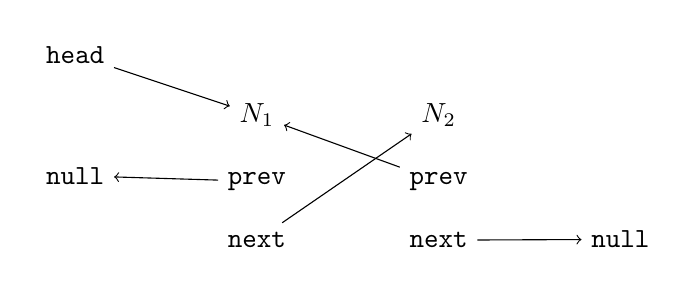
\begin{tikzpicture}
\matrix (m) [matrix of math nodes, row sep=0.8em, column sep=3.8em, minimum width=1.2em]
{
	\texttt{head} & & & \\
	& N_1 & N_2 & \\
	\texttt{null} & \texttt{prev} & \texttt{prev} & \\
	& \texttt{next} & \texttt{next} & \texttt{null} \\
};
\path[->]
(m-1-1) edge node [left] {} (m-2-2)
(m-3-2) edge node [left] {} (m-3-1)
(m-4-2) edge node [left] {} (m-2-3)
(m-3-3) edge node [left] {} (m-2-2)
(m-4-3) edge node [left] {} (m-4-4)
;
\end{tikzpicture} 


You can implement this in the RAM model. A pointer becomes an index into this giant table. In C, do pointer arithmetic to get next element in RAM array.

In this model (pointer machine) you can only follow pointers (costs constant time).

Demaine: RAM model and pointer model are simple, load, store, follow pointer operations take $O(1)$ constant time.

\subsubsection{Python Model}

1. "list" $=$ array (list in Python is an array in RAM).

\begin{verbatim}
L[i] = L[j] + 5	
\end{verbatim}
(takes $O(1)$ time (in Python it's constant time, O(N) for access in a linked list)

2. Object with O(1) attributes

If object has 3 things or 10 things, constant time O(1) operations.

e.g. \verb|x = x.next| is $\Longrightarrow$ O(1) time.

For appending to a list \emph{in Python},

\verb|L.append(x)|

$\Longrightarrow$ \emph{table doubling} (lecture 9) (Python uses an algorithm called table doubling to do appending to a list) \\
$\Longrightarrow$ it's O(1) time 

Demaine: There's a lot more 

\verb|L = L1 + L2| (concatenate 2 lists)

$\equiv $ \verb| L = [] | \\

\verb|for x in L1:| \quad \quad \, O(L1) time \\
\verb|  L.append(x) // O(1) time|
\verb|for x in L2:| \quad \quad \, O(L2) time \\
\verb|  L.append(x) // O(1) time|

In total, O(|L1| + |L2|) time.

Demaine: don't think addition operation sign $+$ means O(1); L1, L2 are large data structures, not words.

\verb|x in L| operation in Python is O(N) worse case is testing every element. \\

\verb|len(L)| O(1): Python stores length of list in beginning. \\

\verb|L.sort()| $\Longrightarrow$ $O(|L| \log{ |L|}) * $ time to compare 2 times.  (Lecture 3; Python uses comparison sort) \\

Python dictionaries, \textbf{dict}.

\verb|D[key]| $=$ val $\Longrightarrow$ O(1) (it's a hash table, lectures 8-10)

Also, alternative syntax: \verb|key in D| \\

Note from Demaine: it's constant time with high probability w.h.p. \\

Demaine: \emph{If you write any code today, use dictionaries to solve problems.} \\

\textbf{long} long integers in Python 3 version 2 (lecture 11) \\

How long does it take to add longs? \\
$x+ y$ \quad \, O(|x| + |y|) \quad \, (EY: think of addition in arithmetic and digit by digit addition)  \\

$x * y$ \quad \, $O((|x| + |y|)^{\log_2{3}})$  Demaine's notation $lg \equiv \log_2$. Now $\lg{3} \approx 1.6$.

\textbf{heapq} heap. Lecture 4.

Demaine: There are more data structures online on the online notes.

\section{Complexity, Big-$O$}

Also note, let $N = $ number of elements in a collection.
\[
\begin{gathered}
	\log_b{N} = n \leftrightarrow b^n = N \\ 
 N \log_b{N} = n \leftrightarrow b^n = N^N \text{ but rather, use Stirling's approximation: } \\
 N \ln N \cong \log_b{N!} = \sum_{i=1}^N \log_b{i} = n  
\end{gathered}
\]
\[
\begin{gathered}
	O(N\log_b{N}) = O(\log_b{N!}) \text{ via Stirling's approximation: } \ln{N!} = N\ln{N} - N + O(\ln{N})
\end{gathered}
\]

cf. Ch. 3 Growth of Functions, 3.1 Asymptotic notation of Cormen, Leiserson, Rivest, and Stein (2009) \cite{CLRS2009}.

\subsection{$\Theta$-notation - worst case}


Formally, \\
given function $g(n)$, 
\begin{equation}
\Theta(g(n)) := \lbrace f(n) | \exists \, c_1, c_2, n_0 > 0 \text{ s.t. } 0 \leq c_1 g(n) \leq f(n) \leq c_2 g(n) \quad \, \forall \, n \geq n_0 \rbrace 
\end{equation}
Formally, \\
\[
f(n) \in \Theta (g(n)) \text{ but notation abuse } f(n) = \Theta(g(n))
\]
$\Theta$-notation asymptotically bounds function from above and below.

\subsection{O-notation - upper bound}

Use O-notation for \textbf{asymptotic upper bound}.

Given function $g(n)$, 
\begin{equation}
O(g(n)) = \lbrace f(n) | \exists \, \text{ positive constants } c, n_0 \text{ s.t. } 0 \leq f(n) \leq c g(n), \quad \, \forall \, n \geq n_0 \rbrace 
\end{equation}
Since for given $f(n) \in \Theta(g(n))$ (abuse notation $f(n) = \Theta(g(n))$, 
\[
\begin{gathered} 
\exists \, c_2, n_0 > 0 \text{ s.t. } f(n) \leq c_2 g(n) \quad \, \forall \, n \geq n_0, \\
f(n) \in O(g(n)) \\
\Longrightarrow \Theta(g(n)) \supseteq O(g(n))
\end{gathered}
\]

$\Omega$-notation, lower bound.

$\Omega$-notation for \textbf{asymptotic lower bound}.

\begin{equation}
\Omega(g(n)) = \lbrace f(n) | \exists \, c, n_0 >0 \text{ s.t. } 0 \leq cg(n) \leq f(n) \quad \, \forall \, n \geq n_0 \rbrace 
\end{equation}

Clearly,
\begin{theorem}[3.1 Cormen, Leiserson, Rivest, and Stein (2009) \cite{CLRS2009}]
$\forall \, $ functions $f(n), g(n)$, $f(n) \in \Theta(g(n))$ iff $f(n) \in O(g(n))$, and $f(n) \in \Omega(g(n))$
\end{theorem}


cf. Demaine and Devadas (2011) \cite{DeDe2001}, \href{https://youtu.be/HtSuA80QTyo}{1. Algorithmic Thinking, Peak Finding, MIT OCW MIT 6.006 Introduction to Algorithms, Fall 2011}. Sept. 8, 2011. PS 1.

\problemhead{PS1, 1-1} \textbf{Asymptotic Practice}

\textbf{Group 1:}

$$
\begin{array}{rcl}
f_1(n) &=& n^{0.999999} \log n \\
f_2(n) &=& 10000000 n \\
f_3(n) &=& 1.000001^n \\
f_4(n) &=& n^2
\end{array}
$$

\textbf{Group 2:}

$$
\begin{array}{rcl}
f_1(n) &=& 2^{2^{1000000}} \\
f_2(n) &=& 2^{100000n} \\
f_3(n) &=& \displaystyle \binom{n}{2} \\
f_4(n) &=& n \sqrt{n}
\end{array}
$$

\solutionhead{1-1, Group 2}

Now
\[
\begin{aligned}
& f_1(n) = 2^{2^{1000000}} = 2^{2^a} \in O(1) \\
& f_2(n) = 2^{100000n} = 2^{Bn} = \exp{(Bn\ln{2})} \\
& f_3(n) = \binom{n}{2} \in O\left( \left( \frac{n}{2} \right)^2 \right) 
\end{aligned}
\]

In general 
\[
\binom{n}{k} \in O\left( \left( \frac{n}{k} \right)^k \right) 
\]

\[
f_4(n) = n \sqrt{n} = n^{3/2} \in O(n^{3/2})
\]

\[
\boxed{
f_1(n) \in O(1) , f_4(n) \in O(n^{3/2}), f_3(n) \in O(n^2) , f_2(n) \in O(2^{Bn})
}
\]


 \textbf{Group 3:}

$$
\begin{array}{rcl}
f_1(n) &=& n^{\sqrt{n}} \\
f_2(n) &=& 2^n \\
f_3(n) &=& n^{10} \cdot 2^{n / 2} \\
f_4(n) &=& \displaystyle\sum_{i = 1}^{n} (i + 1)
\end{array}
$$

\[
\begin{gathered}
	f_4(n) = \sum_{i=1}^n (i + 1) = \sum_{i=1}^n i + \sum_{i=1}^n 1 = \frac{n(n+1)}{2} + n \in O(n^2)
\end{gathered}
\]
\[
\begin{gathered}
	f_1(n) = n^{\sqrt{n}} = n^{n^{1/2}} \\
	\begin{gathered}
		y = n^{n^{1/2}} \\
		\lg{y} = n^{1/2} \lg{n} \\
	y = 2^{n^{1/2} \lg{n}}
	\end{gathered} \quad \quad \, \begin{gathered}
	\ln{y} = n^{1/2} \ln{n} \\ 
	y = \exp{ (n^{1/2} \ln{n})}
	\end{gathered}
\end{gathered}
\]

\[
\begin{gathered}
	f_2(n) = 2^n = \exp{(n\ln{2})}
\end{gathered}
\]

In changing the constant of the function in the \emph{exponent is the same as changing the base of the component}, which does affect asymptotic running time.

\[
\begin{gathered}
f_3(n) = n^{10} \cdot 2^{n/2} \\
\begin{gathered}
y = n^{10} \cdot 2^{n/2} \\
\lg{y} = 10 \lg{n} + \frac{n}{2} \\
y = 2^{10 \log{n} + n/2}
\end{gathered}
\quad \quad \, \begin{gathered}
\ln{y} = 10 \ln{n} + \frac{n}{2} \ln{2} \\
y = \exp{(10 \ln{n} + \frac{ \ln{2}}{2} n )}
\end{gathered}
\end{gathered}
\]

So in order of increasing complexity,

\[
\boxed{
\begin{aligned}
& f_4(n) \in O(n^2) \\
& f_1(n) \in O(2^{n^{1/2} \lg{n}}) \subset O(2^n) \\
& f_3(n) \in O(2^{n/2 + 10 \lg{n}}) \subset O(2^{n/2}) \\
& f_2(n) \in O(2^n)
\end{aligned}
}
\]


\subsection{Multi-Part Algorithms: Add vs. Multiply, e.g. $O(A + B)$ vs. $O(A*B)$}

If your algorithm is "do this ($A$), then, when completed, do that ($B$)" then add runtimes: $O(A+B)$.

If your algorithm is "do this for each time you do that", then multiply runtimes: $O(A*B)$.

\subsection{Amoritized Time (e.g. dynamically resizing array "ArrayList" or maybe \texttt{std::vector})}

Dynamically resize array $x$: if there are $N$ elements, s.t. $N= $ max. capacity at $N$, $|x| = N \mapsto |x| = 2N$ and there are $N$ copies to be made ($T=N$). 

Let $X = $ number of elements to be inserted. 

Suppose when $x=1, 2, 4, 8, 16, \dots 2^j, \dots X$, $x= 2^j$ copies are made. 

total number of copies:
\[
\begin{gathered}
\sum_{j=0}^{ \lfloor \log_2{X} \rfloor } 2^j = \sum_{j=0}^{ \lfloor \log_2{X} \rfloor } 2^{ \lfloor \log_2{X} \rfloor - j} = \sum_{j=0}^{ \lfloor \log_2{X} \rfloor } \frac{X}{2^j} = X\left( \frac{ 1 - 2^{ - (\lfloor \log_2{X} \rfloor  + 1)} }{ 1 - 1/2} \right) = 2X \left( 1 - 2/X \right) \\
\cong 2X \text{ if $X$ large } 
\end{gathered}
\]
Note that $\begin{aligned} & \quad \\ 
 X & = 2^y \\ 
 \log_2{X} & = y \end{aligned}$ 
 
 $X$ insertions take $O(2X)$.  "Amoritized" time for each insertion is $O(1)$.
 
\subsection{$\log{N}$ runtimes ($O(\log{N})$)} 

e.g. binary search. find element (example) $c$ in $N$-element \emph{sorted} array. $x= x_i$, $i=0,1, \dots N-1 \mapsto i' = 1, 2 \dots N$. 

First, compare $c$ to midpoint of array. 

If $c= x_{ \lceil \frac{N}{2} \rceil }$, done.

So let $n_1 =N$.  \\

if $c< x_{ \lceil \frac{N}{2} \rceil }$, consider $x_1, x_2, \dots x_{ \lfloor \frac{N}{2} \rfloor }$, if $c> x_{ \lceil \frac{N}{2} \rceil }$, consider $x_{ \lceil \frac{N}{2} \rceil + 1},  \dots x_N$ \\
 
Let $n_2= \lfloor \frac{N}{2} \rfloor$. 

By induction, $n_j = \lfloor \frac{N}{2^{j-1}} \rfloor$

We stop when we either find the value $c$ or we're down to just 1 element. \\
$\Longrightarrow $ total runtime is the a matter of how many steps (dividing $N$ by 2 each time).

$J = ?$ s.t. $n_J = 1 = \lfloor \frac{N}{2^{J-1}} \rfloor \Longrightarrow  0 = \log_2{N} + (-J + 1)$ or 
\[
J = \log_2{N}
\]
When you see a problem where number of elements $n_0 = N, \dots n_j$ gets halved each time, it'll likely be $O(\log_2{N})$ runtime. 

Finding an element in a \textbf{balanced binary search tree}: $O(\log{N})$; with each comparison, we go either left or right.

\subsection{Recursive run times $O(2^N)$}

\[
\begin{gathered}
	\begin{aligned}
	\text{ Let } & n_1 = N \\
	& n_2 = N - 1 \\
	& \dots  \\
	& n_j = N - j + 1 \\
	& \text{ until } j = N 
	\end{aligned} \qquad \mapsto \qquad 
	\begin{aligned}
	& 2^1 \quad \, f(n_1 - 1) = f(N-1) \text{ calls } \\ 
	& 4 = 2^2 \quad \, f(n_2- 1) \text{ calls }  \\
	& \dots \\
	& 2^j \quad \, f(n_j - 1) \text{ calls }  \\
	& 2^N 
	\end{aligned}
\end{gathered}
\]
\[
\begin{gathered}
	\sum_{j=1}^N 2^j = \sum_{j=0}^{N-1} 2^{N-j} = 2^N \sum_{j=0}^{N-1} 2^{-j} = 2^N \left(\frac{ 1 - 2^{-N} }{ 1 - 1/2} \right) = 2^{N+1} (1- 2^{-N}) \cong 2^N \qquad \, (N \text{ large }) \\ 
 \Longrightarrow 2^{N+1} -1 \text{ nodes } 
\end{gathered}
\]

Try to remember this pattern. When you have a recursive function that makes multiple calls, runtime will often (not always) look like
\begin{equation}
	\boxed{ O(\text{branches}^{\text{depth}}) }
\end{equation}
branches $=$ number of times each recursive call branches.

space complexity is $O(N)$, only $O(N)$ nodes exist at any time.

cf. VI Big O, pp. 46, McDowell, Example 1

\begin{verbatim}
for (int i=0; i < N; i++)
{ sum += array[i]; }
\end{verbatim}
$O(N)$.

cf. VI Big O, pp. 46, McDowell, Example 2

\begin{verbatim}
for (int i = 0; i < N; i++)
{
	for (int j = 0; j < N; j++)
	{
		std::cout << i << j;
	}
}
\end{verbatim}

$O(N*N)= O(N^2)$ Or see it as printing $O(N^2)$ total number of pairs.

cf. VI Big O, pp. 46, McDowell, Example 3
\begin{verbatim}
for (int i = 0; i < N; i++)
{
	for (int j = i + 1; j < N; j++)
	{
		std::cout << i << j;
	}
}
\end{verbatim}
\[
\begin{gathered}
	\begin{aligned}
	& i = 1, 2 \dots N \\
	& j = i+1, \dots N \\
	& \sum_{j=i+1}^N 1 = N-i 
	\end{aligned} \\
\sum_{i=1}^N (N-i) = N\cdot N  - \sum_{i=1}^N i = N^2 - \frac{N(N+1)}{2} = N^2 - \frac{N^2}{2} - \frac{N}{2} = \frac{N^2 - N}{2} \cong N^2 \quad \, \text{(large)}
\end{gathered}
\]

cf. VI Big O, pp. 46, McDowell, Example 4
\begin{verbatim}
for (int i = 0; i < NA; i++)
{
	for (int j = i + 1; j < NB; j++)
	{
		if (a[i] < b[j])
		{
			std::cout << a[i] << b[j];
		}
	}
}
\end{verbatim}
if statement within $j$'s for loop is $O(1)$ time since it's just a sequence of constant time statements.

$\Longrightarrow O(NA \cdot NB)$

cf. VI Big O, pp. 47, McDowell, Example 5

\begin{verbatim}
for (int i = 0; i < NA; i++)
{
	for (int j = i + 1; j < NB; j++)
	{
		for (int k = 0; k < 1000000; k++) 
		{
		//...
		}
	}
}
\end{verbatim}

$\Longrightarrow O(NA \cdot NB \cdot 1000000) = O(100000 (NA)(NB)) \cong O(NA\cdot NB)$

100,000 units of work is still constant, so run time is $O(NA\cdot NB)$.

cf. VI Big O, pp. 48, McDowell, Example 6

\begin{verbatim}
void reverse(int array[], const int N)
{
	for (int i = 0; i < N / 2; i++)
	{
		int other = N - i - 1;
		int temp = array[i];
		array[i] = array[other];
		array[other] = temp;
	}
}
\end{verbatim}
$O(N)$ time. The fact that it only goes through half of the array (in terms of iterations) doesn't impact big O time.

cf. VI Big O, pp. 47, McDowell, Example 8

Let the longest string be of length $L$. \\
sort each string $\to L\log{L}$ (merge sort or best "worst" case for a sort) \\
$N_a= $ number of strings in the array of strings. \\
$N_a L \log{L} = $ total number of sorts. \\

Sort the full array.\\
\emph{You should also take into account that you need to compare the strings.} \\
\emph{Each string comparison takes $O(L)$ time (compare each string element at each position)}. \\
$O(N_a \log{N_a})$ comparisons (sort the full array of strings) \\

\[
\Longrightarrow \boxed{ O(N_a L \log{L}) + O(L N_a \log{N_a}) = O(N_aL (\log{LN_a})) }
\]



\section{Data Structures}

\subsection{Lists (arrays), Python Lists}

cf. \url{https://wiki.python.org/moin/TimeComplexity}, from 4. Quiz: Python Lists, Lesson 2: List-Based Collections, Udacity, \href{https://classroom.udacity.com/courses/ud513/lessons/7117335401/concepts/78894523130923}{Data Structures and Algorithms in Python}
\begin{center}
	\begin{tabular}{ l | c | r }
		\hline
		Operation & Average & Amoritized Worst Case \\ \hline
		Copy & $O(N)$ & $O(N)$ \\ \hline
		Append(1) & $O(1)$ & $O(1)$ \\ \hline
		pop last & $O(1)$ & $O(1)$ \\ \hline
		insert & $O(N)$ & $O(N)$ \\ \hline
		Get item & $O(1)$ & $O(1)$ \\ \hline
		Set item & $O(1)$ & $O(1)$ \\ \hline
		Delete item & $O(N)$ & $O(N)$ \\ \hline
		Get slice & $O(k)$ & $O(k)$ \\ \hline		
		\emph{Get length} & O(1) & O(1) \\ \hline
		\hline
	\end{tabular}
\end{center}

Insert and delete is $O(N)$. Need to move every element with index greater than $k$, and reindex each element.

Get array length is $O(1)$. cf. \url{https://stackoverflow.com/questions/21614298/what-is-the-runtime-of-array-length} 



\subsection{Linked Lists, $O(1)$ insertion}

\subsubsection{Linked Lists vs. arrays}

main difference: Linked lists and arrays store difference information in each element. \\

Both cases: each element stores a value. \\
Both cases: stores 1 more information. \\

Array: index as a number. \\
Linked List: reference to next element, e.g. store addresses of next element, e.g. $x0123$ \\
e.g.
\[
\begin{gathered}
\begin{gathered}
x0122 \\
\text{value}: 8 \\
\text{next}: x0123
\end{gathered} \qquad \qquad \, 
\begin{gathered}
x0122 \\
\text{value}: 8 \\
\text{next}: \text{nullptr}
\end{gathered}
\end{gathered}
\]
Trick to remember: Given elements at addresses 1, 2, 3. If you delete the next reference for 1 (to 2), and replace it with a new object, you'll lose your reference to 3. \\
Assign your next reference to object at 2 before assigning next reference to 1.

Insertion takes constant time since you're just shifting around (constant, finite number of) pointers, instead of iterating every element of the list.

Doubly linked list: Also have pointers to previous element, e.g.
\[
\begin{gathered}
\begin{gathered}
1 \\
\text{value:} 8 \\
\text{next:} 2 \\
\text{prev:} 0
\end{gathered} \qquad \, 
\begin{gathered}
2 \\
\text{value:} 2 \\
\text{next:} 3 \\
\text{prev:} 1
\end{gathered} \qquad \, 
\begin{gathered}
3 \\
\text{value:} 6 \\
\text{next:} 4 \\
\text{prev:} 2
\end{gathered}
\end{gathered}
\]

cf. \url{https://en.wikipedia.org/wiki/Linked_list}

Disadvantages of Linked Lists:
\begin{itemize}
	\item Use more memory than arrays because storage used by their pointers
	\item Nodes in linked list must be read in order from beginning: inherently sequential access
	\item nodes stored in continguously (possibly)
	\item difficult to reverse traverse, doubly linked list helps, but memory consumed in allocating space for back-ptr
\end{itemize}

Linked lists vs. dynamic arrays: \\
List data structures comparison \\

\begin{center}
	\begin{tabular}{ l | c | c | c | c | p{50pt} }
		\hline
		& Linked list & Array & Dynamic Array & Balanced Tree & Hashed \newline array tree \\ \hline 
		indexing & $O(N)$ & $O(1)$ & $O(1)$ & $O(\log{N})$ & $O(1)$ \\ \hline 
		insert/delete at beginning & $O(1)$ &  & $O(N)$ & $O(\log{N})$ & $O(N)$ \\ \hline 
		insert/delete at end & $\begin{gathered} O(1) \text{ when last element is known } \\ O(N) \text{ when last element is unknown }\end{gathered}$ &  & $O(1)$ amoritized  & $O(\log{N})$  & $O(N)$ \\ \hline 
		insert/delete in middle & search time $+ O(1)$ &  & $O(N)$ & $O(\log{N})$ & $O(N)$ \\ \hline 
		wasted space (average) & $O(N)$ & 0  & $O(N)$ & $O(\log{N})$ & $O(\sqrt{N})$ \\ \hline 
		\hline
	\end{tabular}
\end{center}

head of list is 1st. node. \\
tail of 1st. last node in 1st. (or rest of list)

cf. pp. 237-238 of Ch. 10 "Elementary Data Structures" of Cormen, Leiserson, Rivest, and Stein (2009) \cite{CLRS2009}.

Given element $x$ in the list, \\
if \verb|x.next| $=$ NIL, element $x$ has no successor and is therefore the last element or \textbf{tail} of the list.

In a circular list, the prev pointer of the head of the list points to tail, and next pointer of the tail of the list points to the head.

\subsubsection{Inserting into a Linked List, $O(1)$ in front}

Given an element $x$ whose key attribute has already been set, LIST-INSERT "splices" $x$ onto front of linked list.

\subsubsection{Deleting from a Linked List, O(1) if given pointer, or O(N) if given key}

LIST-DELETE removes element $x$ from linked list $L$. \\
It must be given a pointer to $x$, and it then "splices" $x$ out of the list by updating pointers. O(1). \\

If we wish to delete an element with a given key, we must first call LIST-SEARCH to retrieve a pointer to the element. O(N) because we need to do a search.

\subsubsection{Sentinel}

Code for LIST-DELETE would be simpler if we can ignore boundary conditions at head and tail of the list: \\

LIST-DELETE'(L, x) \\
\quad x.prev.next $=$ x.next \\
\quad x.next.prev $=$ x.prev \\

instead of  \\

if x is not head, \\
\quad x.prev.next $=$ x.next \\
else \\
\quad L.head $=$ x.next \\
if x is not tail \\
\quad x.next.prev = x.prev \\

\textbf{Sentinel} is a dummy object that allows us to simplify boundary conditions.

Wherever we have NIL in the code, replace it by sentinel L.nil. \\
e.g. changes doubly linked list into a circular, doubly linked list with sentinel. \\
sentinel L.nil lies between head and tail. \\
attribute L.nil.next points to head of the list, \\
L.nil.prev points to tail. \\
Similarly, \emph{next} attribute of tail and \emph{prev} attribute of head point to L.nil \\

Since L.nil.next points to head, we can eliminate attribute L.head altogether.

\exercisehead{10.2-1, Cormen, Leiserson, Rivest, and Stein (2009) \cite{CLRS2009}}

\emph{Can you implement the dynamic-set operation INSERT on a singly linked list in $O(1)$ time? How about DELETE?}

cf. 3.05.\verb|Linked_lists.pptx| of  Harder (2018) \cite{Hard2018}, assign to the head a new node with the target value and pointing to the previous head, for its next attribute/field. 

To delete, assign a temporary pointer to point to the node being deleted. Then assign head to its next attribute/field. Then delete the temporary pointer that pointed to the original head.

\exercisehead{10.2-2, Cormen, Leiserson, Rivest, and Stein (2009) \cite{CLRS2009}}

\emph{Implement a stack using a singly linked list $L$. The operations PUSH and POP should still take $O(1)$ time.}

PUSH is exactly push front for a linked list. POP is exactly pop front for a linked list. To repeat, push front is assign to head a new node with target value and next attribute/field pointing to original head. pop front is first check if it's empty. If not, then assign a temporary pointer to the head node being deleted. Then assign to head its next. Then delete what the temporary pointer points to.

\exercisehead{10.2-3, Cormen, Leiserson, Rivest, and Stein (2009) \cite{CLRS2009}}

\emph{Implement a queue by a singly linked list $L$. The operations ENQUEUE and DEQUEUE should still take $O(1)$ time}.

Keep a pointer to last element in linked list, as well as the head pointer. \\
To enqueue, insert element after last element of the list, and set it to new, last element (tail). \\
To dequeue, pop front, i.e. delete first element of list and return it. \\

\exercisehead{10.2-7, Cormen, Leiserson, Rivest, and Stein (2009) \cite{CLRS2009}}

\emph{Given a $\Theta(n)$-time nonrecursive procedure that reverses a singly linked list of $n$ elements. The procedure should use no more than constant storage beyond that needed for the list itself.} \\

current $=$ L.head.next \\
previous $=$ L.head \\
while current $\neq$ nullptr, \\
\quad next $=$ current.next \\
\quad current.next = previous (does the actual reversing) \\
\quad previous = current \\
\quad current = next \\
L.head = previous \\

cf. \url{https://sites.math.rutgers.edu/~ajl213/CLRS/Ch10.pdf}

\problemhead{10-1, Comparisons among lists, Cormen, Leiserson, Rivest, and Stein (2009) \cite{CLRS2009}}

\begin{center}
	\begin{tabular}{ l | c | c | c | c }
		& unsorted, singly linked & sorted, singly linked & unsorted, doubly linked & sorted, doubly linked \\
		SEARCH(L, k) & N & N & N & N \\
		INSERT(L, x) & 1 & 1 & 1 & 1 \\
		DELETE(L, x) & N & N & 1 & 1 \\
		SUCCESSOR(L, x) & N & 1 & N & 1 \\
		PREDECCESSOR(L, x) & N & N & N & 1 \\
		MINIMUM(L) & N & 1 & N & 1 \\
		MAXIMUM(L) & N & N & N & 1\\
	\end{tabular}
\end{center}


\subsection{Implementing pointers and objects for data structures}

cf. Sec. 10.3 "Implementing pointers and objects" in Cormen, Leiserson, Rivest, and Stein (2009) \cite{CLRS2009}.

\subsubsection{A multiple-array representation of objects for linked lists}

3 arrays, array \emph{key} holds values of keys currently in the dynamic set. \\
pointers in arrays \emph{next} and \emph{prev} (notation: \emph{previous}). \\
Given array index $x$ (notation: $i$), key[i], next[i], previous[i] represents an object in the linked list. \\

\subsubsection{Allocating and freeing objects; example of doubly linked list represented by multiple arrays}

Suppose arrays in multiple-array representation have length $m$, and at some moment, dynamic set contains $n\leq m$ elements. \\
Then $n$ objects represent elements currently in the dynamic set, \\
remaining $m-n$ objects are \textbf{free}. \\

Keep free objects in a singly linked list, called \textbf{free list}.

Free list uses only next array, which stores next pointers (i.e. index to next element). 

head of free list held in global variable free. 

free list acts like a stack. \\

Allocate-object(): \\
if free $==$ nil, \\
\quad error "out of space" \\
else $x= $ free \\
\quad free $=$ x.next \\
\quad return x \\

free-object(x) \\
x.next $=$ free \\
free $=$ x \\

\exercisehead{10.3-2, Cormen, Leiserson, Rivest, and Stein (2009) \cite{CLRS2009}}

\emph{Write the procedures Allocate-Object and Free-Object for a homogeneous collection of objects implemented by the single-array representation}.

Single array will act like a stack. Keep a "pointer" to index of last element, $i_{\text{last}}$.  \\

Allocate-Object() \\
if full, throw error \\
else, \\
\quad $++i_{\text{last}}$ \\
\quad return x[$i_{\text{last}}$] \\

free-object() \\
\quad $--i_{\text{last}}$ \\

\exercisehead{10.3-3, Cormen, Leiserson, Rivest, and Stein (2009) \cite{CLRS2009}}

\emph{Why don't we need to set or reset the prev attributes of objects in the implementation of the Allocate-Object and Free-Object procedures?}

Allocate object just returns index of some cells that it's guaranteed to not give out again until they've been freed. 

prev attribute isn't modified because only next attribute is used by memory manager.

In Free-Object procedure, we only need to set free to the given object to free.

cf. \url{https://sites.math.rutgers.edu/~ajl213/CLRS/Ch10.pdf}

\subsection{Stack, $O(1)$ pop, $O(1)$ push}

\href{https://classroom.udacity.com/courses/ud513/lessons/7117335401/concepts/71225347790923}{"Stack Details", Udacity, Data Structures and Algorithms}

top element $\mapsto $ Linked List head \\
push top element, pop top element.
Last in, first out. \\
Last element you put in (new head), is the First out (when you pop).

\subsection{Queue, $O(1)$ insert, $O(1)$ delete, $O(N)$ search, $O(N)$ space complexities}

\url{https://en.wikipedia.org/wiki/Queue_(abstract_data_type)}
\href{https://classroom.udacity.com/courses/ud513/lessons/7117335401/concepts/71222050580923}{Lesson 2: List-Based Collections, 11. Queues}

Oldest element (tail) comes out first.

cf. pp. 121, Sec. 1.3 Bags, Queues, and Stacks, Sedgewick and Wayne (2011) \cite{SeWa2011}

First In, First Out (FIFO). \\
first element you put in (tail) is the first out (when you pop). \\

Applications for Queues: cf. Harder (2018) \cite{Hard2018}, 3.03.Queues.pptx
\begin{itemize}
	\item Queuing clients in a client-server model
	\item Breadth-first traversals of trees, i.e. \emph{use queues for breadth-first traversals of trees}
\end{itemize}

\subsubsection{Queue as Circular Array}

cf. pp. 234, Ch. 10 Elementary Data Structures of Cormen, Leiserson, Rivest, and Stein (2009) \cite{CLRS2009}

\verb|Q.head| attribute that indexes, or points to, its head. \\
\verb|Q.tail| indexes next location at which newly arriving element will be inserted. \\
elements reside in \verb|Q.head|, \verb|Q.head| $+1, \dots \verb|Q.tail| - 1$. When $\verb|Q.head| = \verb|Q.tail|$, queue is empty.

Figure 10.2 of Cormen, Leiserson, Rivest, and Stein (2009) \cite{CLRS2009} shows one way to implement a queue of \textbf{at most $n-1$ elements } using an \textbf{array $Q[1\dots n]$}.  This is an important point: see \href{https://stackoverflow.com/questions/16395354/why-q-head-q-tail-1-represents-the-queue-is-full-in-clrs}{Stack overflow}.

\subsubsection{Queue as Linked List}


head. "oldest element in the queue", "first" \\
tail. "newest element in queue", "last", \\
(I guess it grows from the tail) \\
add element to tail, enqueue. \\
Dequeue, remove head. \\
peek - peek at head. \\

Save references to head and tail.

\exercisehead{10.1-2, Cormen, Leiserson, Rivest, and Stein (2009) \cite{CLRS2009}} \emph{Explain how to implement 2 stacks in 1 array $A[1\dots n]$ in such a way that neither stack overflows unless the total number of elements in both stacks together is $n$. The PUSH and POP operations should run in $O(1)$ time.}

The first stack starts at 1 and grows up towards $n$, while the second stack starts from $n$ and grows down towards $n$. Stack overflow happens when an element is pushed when the 2 stack pointers are adjacent.

\exercisehead{10.1-6, Cormen, Leiserson, Rivest, and Stein (2009) \cite{CLRS2009}} \emph{Show how to implement a queue using 2 stacks. Analyze the running time of the queue operations.} 

For a queue q, recall a queue follows LIFO order. Given 2 stacks, s1, s2, recall stacks are FIFO.

The following are the solutions (implementation): \\
enqueue - enqueue pushes an element into s2. Check if s1 empty. \\
dequeue - dequeue pops elements from s1. Check if s1 empty. \\
If at any time, s1 is empty, then pop all elements in s2, into s1 so that the order is reversed.

Case 0. q empty, so s1 and s2 empty, enqueue element x1. Check if s1 empty then pops x1 into s1. Dequeue pops element x1.

Assume n1, n2 cases for s1, s2. Enqueue pushes x into s2. s1 not empty and still in LIFO order from assumption. Dequeue pops x1 from assumption. If n1 = 1, then n2 + 1 elements from s2 will be popped into s1 in reversed or LIFO order.

Average case time complexity for both is O(1). Worst case time complexity is O(N) because of the transfer from s2 to s1 to maintain LIFO order.

\exercisehead{10.1-7, Cormen, Leiserson, Rivest, and Stein (2009) \cite{CLRS2009}} \emph{Show how to implement a stack using 2 queues. Analyze running time of stack operations}.

For a stack s, given 2 queues, choose 1 queue to be active $q_a$, and another to be not active $q_{na}$.

push: given element x, enqueue into $q_a$. O(1) time. 

Because queues when popping or pushing "preserves order", the only way to get the last element in is to dequeue until the very last element.

pop: dequeue $q_a$ until last element is reached (can check if empty afterwards). Then return that last element. Also, enqueue previous elements into $q_{na}$ and label $q_{na} \mapsto q_a$ to be active.




\subsubsection{Deque. double-ended queue}

One can enqueue and dequeue from either end.

\subsubsection{Priority Queue}. 
Assign each element in queue with a priority. \\
Remove oldest and highest priority element first.

\subsection{STL Containers}

cf. Ch. 31, STL Containers, Bjarne Stroustrup (2013) \cite{Stro2013}

pp. 886 Stroustrup (2013) \cite{Stro2013}
\verb|std::vector<T, A>| contiguous allocated sequence of \verb|T|s;

cf. pp. 888 Sec. 31.2.1 "Container Representation", \cite{Stro2013}

\verb|vector| element data structure is most likely an array:

\verb|vector|: rep $\leftarrow$ elements | free space

\verb|list| : likely represented by sequence of links pointing to elements and number of elements; doubly-linked list of \verb|T|; use when you need to insert and delete elements without moving existing elements.

\verb|map| : likely implemented as (balanced) tree of nodes pointing to (key, value) pairs:

\verb|unordered_map| likely implemented as hash table

\verb|unordered_map| rep $\leftarrow $ hash table $\leftarrow$, $\leftarrow$, $\dots$ (k, v), (k, v) , $\dots$

\verb|string| for short strings, characters are stored in the string handle itself, for longer strings elements are stored contiguously on free-store (like \verb|vector| elements). Like \verb|vector|, \verb|string| can grow into "free space" allocated to avoid repeated reallocations.

\verb|string|: rep $\leftarrow$ characters -- free space

Like a built-in array, \verb|array| is simply sequence of elements, with no handle,
\verb|array|: elements

cf. pp. 894, Sec. 31.3, Operations Overview, Stroustrup (2013) \cite{Stro2013}

Standard Container Operation Complexity
\begin{center}
	\begin{tabular}{ l | l | l | l | l | l }
		\hline
		& \verb|[]| Sec. 31.2.2 & List Sec. 31.3.7 & Front Sec. 31.4.2 & Back Sec. 31.3.6 & Iterators  Sec. 33.1.2 \\ \hline \hline
		\verb|vector| & const & $O(n)+$ &  & const $+$ & Ran \\ \hline 
		\verb|list| &  & const &  const  & const & Bi \\ \hline 
		\verb|forward_list| &  & const &  const  &  & For \\ \hline 
		\verb|deque| & const & $O(N)$ &  const  & const & Ran \\ \hline \hline 
		\verb|stack| &  &  &   & const &  \\ \hline 
		\verb|queue| &  &  & const  & const &  \\ \hline 
		\verb|priority_queue| &  &  & $O(\log{(n)})$  & $O(\log{(n)})$ &  \\ \hline \hline
		\verb|map| & $O(\log{(n)})$ & $O(\log{(n)})+$ & & & Bi \\ \hline
		\verb|set| &  & $O(\log{(n)})+$ & & & Bi \\ \hline
		\verb|unordered_map| & const+ & const$+$ & & & For \\ \hline
		\verb|unordered_set| &  & const$+$ & & & For \\ \hline \hline 
		\verb|string| & const & $O(n)+$ & $O(n)+$ & const$+$ & Ran \\ \hline
		\verb|array| & const &  & & & Ran \\ \hline 	
		\hline
	\end{tabular}
\end{center}
Ran - random-access iterator, "For" - "forward iterator", "Bi" - "bidirectional iterator"

\subsection{vector}

\subsubsection{vector and growth}

Layout of \verb|vector| : elem $\leftarrow$ "front" of elements, \\
space $\leftarrow$ "front" of extra space (meets end of elements) \\
last $\leftarrow$ end of extra space \\
alloc

Use of both size (number of elements), and capacity (number of available slots for elements without reallocation) makes growth through \verb|push_back()| reasonably efficient: there's not an allocation operation each time we add an element, only every time we exceed capacity (Sec. 13.6) \\
adding half the size is common, standard doesn't specify by how much capacity is increased

\subsubsection{vector and Nesting}

\verb|vector| (and similarly contiguously allocated data structures) has 3 major advantages:
\begin{itemize}
	\item elements of \verb|vector| compactly stored; no per-element memory overhead (contiguous on memory address) \\
	amount of memory consumed by \verb|vec| of type \verb|vector<X>| roughly \\
	\verb|sizeof(vector<X>)+vec.size()*sizeof(X)|; \verb|sizeof(vector<X>)| is about 12 bytes, insignificant for large vectors
	\item fast traversal, consecutive access, to get to next element, code doesn't have to indirect through a pointer 
	\item simple and efficient random access, makes sort and binary search efficient
\end{itemize}

vs. doubly-linked list, \verb|list|, incurs 4-words-per-element memory overhead (2 links plus free-store allocation header)

be careful don't unintentional compromise efficiency of access, e.g. 2-dim. matrix \\
don't do \verb|vector<vector<double>>|, \\
do \verb|vector<double>| and compute locations from the indices 

\subsubsection{vector vs. array}

\verb|vector| resource handle, i.e. allows it to be resized and enable efficient move semantics, \\
disadvantage to arrays that don't rely on storing elements separately from handle; keeps sequence of elements on stack or in another object.

\subsection{Trees}

value, left pointer, right pointer,

levels - how many connections it takes to reach the root $+ 1$
child can only have 1 parent
height - number of edges between it and farthest leaf \\
depth - number of edges to root.

height, depth are inverse

\subsubsection{Rooted Trees representation}

cf. Sec. 10.4 "Representing rooted trees", Cormen, Leiserson, Rivest, and Stein (2009) \cite{CLRS2009}

Assume each node contains a key attribute.

\subsubsection{Binary trees representation}

p, left, right store pointers to parent, left child, right child. \\
if x.p = NIL, then x is root \\
if x.left = NIL, node x has no left child. \\
if x.right = NIL, node x has no right child. \\

root of entire tree T is printed to by attribute T.root 

\subsubsection{Rooted trees with unbounded branching}

If (class of) tree has number of children of each node is at most some constant k.

Replace the left, right attributes by child1, child2, ... childk

For arbitrary numbers of children, \textbf{left-child, right-sibling representation} \\
each node has parent pointer p \\
T.root points to root of tree T \\
each node has only 2 pointers \\
1. x.left-child points to left most child of node x \\
2. x.right-sibling points to sibling of x immediately to its right \\

If node x has no children, then x.left-child =NIL \\
If node x is rightmost child of its parent, then x.right-sibling = NIL

\exercisehead{10.4-2, Cormen, Leiserson, Rivest, and Stein (2009) \cite{CLRS2009}}

\emph{Write an $O(n)$-time recursive procedure that, given an $n$-node binary tree, prints out the key of each node in the tree}.

cf. \url{https://sites.math.rutgers.edu/~ajl213/CLRS/Ch10.pdf}

(this is for pre-order)
print-tree(node) \\
if node == NIL, return \\
else \\
\quad print node.key \\
\quad print-tree(node.left) \\
\quad print-tree(node.right) \\

\subsubsection{Preorder, postorder, inorder traversal, recursive}

To reiterate from \href{https://en.wikipedia.org/wiki/Tree_traversal#Depth-first_search}{wikipedia, "Tree Traversal"}, \\

\textbf{preorder traversal} \\
\begin{enumerate}
	\item visit current node
	\item recursively traverse left subtree
	\item recursively traverse right subtree
\end{enumerate}

\textbf{postorder traversal} \\
\begin{enumerate}
	\item recursively traverse left subtree
	\item recursively traverse right subtree
	\item visit current node
\end{enumerate}

\textbf{inorder traversal} \\
\begin{enumerate}
	\item recursively traverse left subtree
	\item visit current node
	\item recursively traverse right subtree
\end{enumerate}

\exercisehead{10.4-3, Cormen, Leiserson, Rivest, and Stein (2009) \cite{CLRS2009}}

\emph{Write an $O(n)$-time nonrecursive procedure that, given an $n$-node binary tree, prints out the key of each node in the tree. Use a stack as an auxiliary data structure}.

printWithStack(node)  \\
let S by an empty stack. \\
push(S, node) \\
while S is not empty, \\
\quad U = pop(S) \\
\quad U $\neq $ NIL, then \\
\quad \quad print U.key \\
\quad \quad push(S, U.left) \\
\quad \quad push(S, U.right) \\

Keep in mind that this \emph{does not} reproduce inorder recursive traversal. This instead exhibits interesting behavior of immediately printing a node. It's because recursion relies on a termination condition, which is typically that a node is a leaf.

\subsubsection{Postorder Traversal with stack}

Consider the following from \href{https://www.geeksforgeeks.org/iterative-postorder-traversal-using-stack/}{geeksforgeeks, iterative postorder}: \\

Create an empty stack. \\
2.1 while root is not NIL, \\
\quad push root's right and then root to stack, \\
\quad set root as root's left child. \\
2.2 pop item from stack and set as root \\
\quad if popped item has right child, and right child is top of the stack, then remove right child from stack, push root back and set root as root's right child \\
\quad else print root's data and set root as nullptr \\
2.3 repeat steps 2.1, 2.2 while stack isn't empty. \\

Consider also the following: \\

Create empty stack S, push(S, node) \\
currentptr=node, previousptr=NIL \\
while S is not empty, \\
\quad currentptr = S.top() \\
\quad if currentptr is a leaf or we've traversed right node of currentptr or left node of currentptr, \\
\quad \quad print currentptr.value \\
\quad \quad S.pop() \\
\quad \quad previousptr = currentptr \\
\quad else \\
\quad \quad if currentptr.right is not NIL, S.push(currentptr.right) \\
\quad \quad if currentptr.left is not NIL, S.push(currentptr.left) \\

The predicate "we've traversed right node of currentptr or left node of currentptr" is to reproduce the recursive stack callback.


\subsection{Graphs}

edges can store data too. \\
Directed graph edges have a sense of direction. \\
$A =$ set of ordered pairs of vertices. \\
undirected graph. \\
acyclic (no cycles) \\
DAG Directed graph with no cycles.

\subsubsection{Connectivity} 

connected graph has only 1 connected component. $\exists \, $ path $\forall \, $ pair of vertices. \\
\qquad \, minimum number of elements (edges) to remove, to disconnect a component. \\

weakly connected directed graph if replacing all its directed edges with undirected edges produces a connected (undirected) graph. 

\subsubsection{Graph Representation} 

vertex object: \\
list of edges. 

Edge Object \\
vertices. 

Edge List: $=E$ 

Adjacency list $l = l(i)$ s.t. $\forall \, i \in V$, $l(i) \in \textbf{Set}$ s.t. $l(i) = $ set of all adjacent vertices. \\

Adjacent Matrix. 

Let $V=$ set of all vertices. \\
$\forall \, v \in V$, label them: $v=v(i)$, $i \in \mathbb{N}$ \\

$\forall \, v_i \in V$, so $\forall \, i = 0, 1, \dots N-1$, \\
Consider $\forall \, w = w_j \in V$, so $\forall \, j = 0 , 1, \dots N-1$. \\

If $v_i, w_j$ are adjacent, let $a(i,j) = 1$, otherwise $w(i,j) =0$. (adjacent means $\exists \,$ edge s.t. $E = \lbrace v_i, w_j \rbrace$) \\
$\Longrightarrow a$ is an adjacency matrix. 

Adjacency list. 

$\forall \, v = v_i \in V$, $i=0,1,\dots N-1$ \\
$E = \lbrace (v_o, v_t) | v_o, v_t \in V \rbrace$ \\
if $\exists \, e \in E$ s.t. $v_i = e(0) = v_o$, then $e(1) = v_t$ is adjacent to it. 

Adjacency list useful for counting number of edges that a node has or number of adjacencies.

\subsubsection{Graph Traversal}  

Depth-first search (DFS) \\
Breadth-first search (BFS) \\

DFS. \\
implementation: stack. \\
keep 2 structures: 1. Seen list, 2. stack. 

If seen before, pop stack and go back. \\
$O(|E| + |V|)$ visit every edge twice $O(2|E| + |V|) = O(|E| + |V|)$. \\
$O(|V|)$ time to look up a vertex. 

More on procedure:

begin with any node $v_1$. Put $v(v_1)$ into seen. Put $v_1$ on stack. \\
if $\exists \, \lbrace e \rbrace \subset E$ s.t. for $e = (v_o, v_t)$ , $v_o = v_1$, then, put $v(v_t)$ into seen. Put $v_t$ on stack.

Then consider $v_t$. \\
If $v(v_t) \in $ seen, consider another edge. \\
If you run out of edges with new node, pop stack. 

Eulerian path $O(|E|) $ 

Hamiltonian path


\subsection{Tries}

Leaves of tree indicate the end of a word.

Each node contains a character of a word. Each branch (path) from child from root to leaf is a word in a collection of words. 

class Nodes $\lbrace $ array of all children or \\
lookup table to do you have child? \\
e.g. HashMap

is end of word

Used in word validation. Given this list of strings, word list validation.
is CA prefix.

Keep state, build on a lookup by keeping state in trie or return by reference to the Node.

\href{https://youtu.be/zIjfhVPRZCg}{Data Structures: Tries, HackerRank}

Insert and search costs O(key length) however, memory requirements of Trie is O(Alphabet size * key length * N) where $N$ is number of keys in Trie.

\section{Searching}

cf. Ch. 9, "Searching", Shaffer (2011) \cite{Shaf2011}.

Suppose we have a collection $\mathbf{L}$ of $n$ records of form
\[
(k_1, I_1), (k_2, I_2) , \dots (k_n, I_n)
\]
where $I_j$ is information associated with key $k_j$ from record $j$ for $1\leq j \leq n$.

Given a particular key value $K$, search problem is to locate record $(k_j, I_j)$ in $\mathbf{L}$ s.t. $k_j = K$ (if one exists). Successful search is 1 in which record with key $k_j = K$ found.




\section{Hash Tables}

\subsection{Direct-address tables}

Direct addressing works well when universe U of keys is small. \\
Suppose dynamic set in which each element has key drawn from universe $U = \lbrace 0 , 1 \dots m - 1 \rbrace$ $m$ not too large. \\
Assume no 2 elements have same key. \\
To represent dynamic set, use array, or \textbf{direct-address table}, $T[0, \dots m-1]$ in which each position, or \textbf{slot}, corresponds to key in universe U. \\
Slot k points to element in set with key k. \\
If set contains no element with key k, then T[k] = NIL \\

Direct-Address-Search(T, k) \\
\quad return T[k] \\

Direct-Address-Insert(T, x) \\
\quad T[x.key] = x \\

Direct-Address-Delete(T,x) \\
\quad T[x.key] = NIL \\

O(1) time.

\exercisehead{11.1-1, Cormen, Leiserson, Rivest, and Stein (2009) \cite{CLRS2009}}

\emph{Suppose that a dynamic set S is represented by a direct-address table T of length m. Describe a procedure that finds the maximum element of S. What is the worst-case performance of your procedure?}

Start at i = m-1. Consider T[i]. $\forall \, m - 1, m- 2, \dots 0$, until T[i] is an element O(m).

\exercisehead{11.1-2, Cormen, Leiserson, Rivest, and Stein (2009) \cite{CLRS2009}}

\emph{A \textbf{bit vector} is simply an array of bits (0s and 1s). A bit vector of length m takes much less space than an array of m pointers. Describe how to use a bit vector to represent a dynamic set of distinct elements with no satellite data. Dictionary operations should run in O(1) time.}

Let x be a bit vector of length $m$. Let dynamic set of n elements s.t. $n\leq m$ of distinct elements with key values from $0, 1, \dots n-1$. \\

insert(k) \\
\quad x[k] = 1\\

Delete(k) \\
\quad x[k] = 0\\

search(k) \\
\quad return x[k] \\

cf. 11.2 "Hash Tables" of Cormen, Leiserson, Rivest, and Stein (2009) \cite{CLRS2009}

Let K of keys stored in dictionary much smaller than universe U of all possible keys, we can reduce storage requirements to $\Theta(|K|)$, while search requires only O(1) time. \\

Given an element with key k, \\
direct addressing: k stored in slot k \\
hashing: element stored in slot H(k), i.e. \textbf{hash value} h(k) of key k \\
hash function $\begin{aligned} & \quad \\ 
& h : U \to \lbrace 0, 1, \dots m -1 \rbrace \\
& h:k \mapsto h(k) \end{aligned}$ s.t. T[h(k)] = k \\

where size m of hash table typically m $< |U|$ \\

\textbf{collision}: 2 keys may hash to same slot. 

\subsubsection{Collision resolution by chaining for Hash Tables}

\textbf{chaining}- place all elements that hash to same slot into same linked list. \\
slot j contains pointer to head of list of all stored elements that hash to j \\
if there are no such elements, slot j contains NIL. \\

Dictionary operations: \\
Chained-Hash-Insert(T,x) \\
\quad insert x at head of list T[j(x.key)] \\

Chained-Hash-Search(T, k) \\
\quad search for element with key k in list T[h(k)] \\

Chained-Hash-Delete(T, x) \\
\quad delete x from list T[h(x.key)] \\

 
For searching, worst-case running time is O(N). \\
Delete an element in O(1) time if list doubly linked. If lists only singly linked, then first have to find x.
 
\subsubsection{Analysis of hashing with chaining}
 
Given hash table T with m slots, stores n elements, define \textbf{load factor} $\alpha := \frac{n}{m}$, i.e. average number of elements stored in chain.

\textbf{simple uniform hashing} - assumption that any given element is equally likely to hash into any of m slots.

$\forall \, j = 0, 1, \dots m - 1$, let length of list T[j] $\equiv n_j$, so that \\
\[
n = n_0 + n_1 + \dots + n_{m-1}
\] 

expected value of $n_j \equiv E[n_j] = \alpha = \frac{n}{m}$ \\

\begin{theorem}[11.1, Cormen, Leiserson, Rivest, and Stein (2009) \cite{CLRS2009}]
In hash table in which collisions are resolved by chaining, unsuccessful search takes average case time $\Theta(1+\alpha)$, under assumption of simple uniform hash.
\end{theorem}

\begin{proof}

By simple uniform hashing assumption, any key k not already stored is equally likely to hash to any m slots.

Expected time to search unsuccessfully for key k is expected time to search to end of list T[h(k)], which has expected length $E[n_{h(k)}] = \alpha$. \\

Thus expected number of elements examined is unsuccessful search is $\alpha$. \\
$\Longrightarrow $ take time required $\Theta(1+\alpha)$
\end{proof}


\begin{theorem}[11.2, Cormen, Leiserson, Rivest, and Stein (2009) \cite{CLRS2009}]
In a hash table in which collisions resolved by chaining, successful search takes average-case time $\Theta(1+\alpha)$, under simple uniform hashing assumption.	
\end{theorem}
\begin{proof}
Assume element being searched equally likely to be any of the n elements stored in table. \\
number of elements examined during successful sesarch for x is 1 more than number of elements that appear before x in x's list. \\
Let $x_i \equiv i$th element inserted into table, $i = 1, 2, \dots n$ \\
\phantom{Let } $k_i \equiv x_i$.key \\

$\forall \, $ keys $k_i, k_j$, define indicator random variable $X_{ij} = I\lbrace h(k_i) = h(k_j) \rbrace$ \\
under simple uniform hashing assumption, $Pr\lbrace h(k_i) = h(k_j) \rbrace = \frac{1}{m}$, because probability to hash into any slot is $\frac{1}{m}$ and so probability to hash into this particular slot is also $\frac{1}{m}$ since it must be as equally likely as any other. \\

$E[X_{ij}] = \frac{1}{m}$ since Lemma 5.1 of Cormen, Leiserson, Rivest, and Stein (2009) \cite{CLRS2009} which is, recall, really simple: $E[X_{ij}] = 1 \cdot Pr\lbrace h(k_i) = h(k_j) \rbrace + 0 \cdot Pr\lbrace h(k_i) = h(k_j) \rbrace$. \\

Note that because new elements placed at front of list, elements before x in list inserted after x inserted. \\

Take average, over n elements in table, of 1 plus expected number of elements added to x's list after x was added to list.

Thus, expected number of elements examined in a successful search,
\[
\begin{gathered}
E\left[ \frac{1}{n} \sum_{i=1}^n \left( 1 + \sum_{j={i+1}}^n X_{ij} \right) \right] = \frac{1}{n} \sum_{i=1}^n \left( 1 + \sum_{j=i+1}^n E[X_{ij}] \right) = \frac{1}{n} \sum_{i=1}^n \left( 1 + \sum_{j=i+1}^n \frac{1}{n} \right) = 1 + \frac{1}{nm} \sum_{i=1}^n (n-i) = \\
= 1 + \frac{n}{m} - \frac{1}{nm} \left( \frac{n (n+1) }{2} \right) = 1 + \frac{n-1}{2m} = 1 + \frac{\alpha}{2} - \frac{\alpha}{2n}
\end{gathered}
\]

Thus total time required for successful search is $\Theta\left(2 + \frac{\alpha}{2} - \frac{\alpha}{2n}\right) = \Theta(1+\alpha)$

\end{proof}

\exercisehead{11.2-1, Cormen, Leiserson, Rivest, and Stein (2009) \cite{CLRS2009}}

cf. \url{https://sites.math.rutgers.edu/~ajl213/CLRS/Ch11.pdf}

Given n distinct keys, suppose keys are totally ordered $\lbrace k_1, \dots k_n \rbrace$. Given key $k_i$, consider $\forall \, l $ s.t. $l > k_i$ and $h(l) = h(k_i)$, \, $Pr[h(l)=h(k)] =\frac{1}{m}$. \\

Probability that for some key there's a collision, 
\[
\sum_{i <j}^n Pr[h(k_j) = h(k_i)] = \sum_{j > i} \frac{1}{m} = \frac{n-i}{m}
\]
Using simple uniform hashing assumption.

Expected number of collisions 
\[
\sum_{i=1}^n \frac{n-i}{m} = \frac{n^2 - \frac{n(n+1)}{2} }{m} = \frac{n (n-1) }{m}
\]

The hash process: 

\[
\begin{gathered}
	\begin{tikzpicture}
		\matrix (m) [matrix of math nodes, row sep=2.8em, column sep=4.8em, minimum width=2.2em]
		{
			\text{Object} & & \\
			\text{32-bit integer} & & \\
			\text{Map to an index } 0, \dots M - 1 & & \\ 
			\text{Deal with collisions} & & \\
			& \text{Linear probing} & \text{Chained hash tables} \\
			& \text{Quadratic probing} & \text{Open addressing} \\
			& \text{Double Hashing} & \\
		};
		\path[->]
		(m-1-1) edge node [auto] {$$} (m-2-1)
		(m-2-1) edge node [right] {Modulus, mid-square, multiplicative, Fibonacci} (m-3-1)
		(m-3-1) edge node [auto] {$$} (m-4-1)
		(m-5-3) edge node [auto] {$$} (m-5-2)
		;
	\end{tikzpicture}   \\
\end{gathered}
\]

\subsection{Hash functions}

cf. 11.3 "Hash functions" of Cormen, Leiserson, Rivest, and Stein (2009) \cite{CLRS2009}

\subsubsection{What makes a good hash function?}

A good hash function satisfies (approximately) assumption of simple uniform hashing: that each key equally likely to hash to any of m slots, independently of where any other key hashed to. \\
Unfortunately, probability distribution from which keys drawn unknown, and drawing itself might not be independent. \\

However, if we know keys are random real numbers k independently, uniformly distributed in range $0\leq k < 1$, then
\begin{equation}
h(k) = \lfloor km \rfloor
\end{equation}
satisfies condition of simple uniform hashing.

Create well-performing hash function: \\
e.g. consider compiler's symbol table, in which keys are character strings, representing identifiers in a program. Closely related symbols, e.g. pt and pts, often occur in same program. \\
- good hash function would minimize change such variants hash to the same slot. \\

A good approach derives hash value independent of patterns that might exist in data: \\
e.g. "division method"; key divided by prime number $\mapsto$ remainder; choose prime number unrelated to problems in keys distribution. \\

example: want keys that are "close" to yield hash values far apart; e.g. universal hashing (11.3.3 of Cormen, Leiserson, Rivest, and Stein (2009) \cite{CLRS2009}).

\subsubsection{Interpreting keys as natural numbers for hash functions}

Most hash functions assume universe of keys is set $\mathbb{N} = \lbrace 0, 1,2, \dots \rbrace$ of natural numbers; thus if keys aren't natural numbers, find a way to interpret as natural numbers. \\
e.g. interpret a character string as integer expressed in suitable radix notation. \\
e.g. pt as p = 112, t = 116, radix-128 int $\mapsto (112 \cdot 128) + 116 = 14452$, i.e.
\[
r(s) = \sum_{j=0}^{N- 1} 128^j \cdot s[j]
\]

\subsubsection{Division method}

map key k into m slots by taking remainder of k divided by m, i.e. 
\begin{equation}
h(k) = k \mod{m}
\end{equation}

m shouldn't be power of 2, since if $m=2^p$, h(k) is just p lowest-order bits of k \\
Unless we know all low-order p bit patterns equally likely better off designing hash function to depend on all bits of key. \\
Exercise 11.3-3 (of Cormen, Leiserson, Rivest, and Stein (2009) \cite{CLRS2009}) shows choosing $m=2^p - 1$ when k is character string interpreted in radix $2^p$ maybe poor choice, because permuting characters of k doesn't change hash value. \\

prime not too close to exact power of 2 often good choice for m \\
e.g. hash table, with collisions resolved by chaining, to hold n = 2000 character strings, where a character has 8 bits = 1 byte \\
We don't mind examining average of 3 elements in an unsuccessful search, so allocate hash table of size m = 701.  \\
Choose m= 701 because it's a prime near $2000/3$ but not near any power of 2
\begin{equation}
h(k) = k \mod{701}
\end{equation}

\subsubsection{Multiplication method}

\[
h(k) = \lfloor m (kA \mod{1}) \rfloor
\]
where $0 < A < 1$, where $kA \mod{1}$ means take the fractional part of $kA$, i.e. $kA - \lfloor kA \rfloor$ \\

advantage of multiplication method: value of $m$ is not critical. \\
typically choose m to be a power of 2 ($m = 2^p$ for some $p \in \mathbb{Z}$). \\

Suppose word size of machine is $w$ bits, $k$ fits into single word. \\

Restrict A to be fraction of form $s/2^w$, where $s$ is an integer in range $0 < s < 2^w$.  \\

So $k \times s = k \times A \cdot 2^w$, \\
where first multiply k by w-bit integer s $= A \cdot 2^w$.  \\

Result is $2w$ bit value $r_1 2^w + r_0$ where $r_1$ is high-order word of product, $r_0$ is low-order word of product desired $p$-bit hash value consists of p most significant bits of $r_0$. \\

Although this method works with any value of constant $A$, optimal choice depends on characteristics of data being hashed. Knuth suggests
\[
A \approx (\sqrt{5} - 1) / 2 = 0.6180339887
\]

e.g. $k= 123456, \, p = 14$ (14-bit has value), $m = 2^{14} = 16384, \, w = 32$ (32-bit word size).

Adapting Knuth's suggestion, choose $A = s/2^w$, and $A \approx (\sqrt{5} - 1) / 2$, so $A = 2654435769 / 2^{32}$. \\
$ k \cdot s = 327706022297664 = (76300 \cdot 2^{32}) + 17612864$, so $r_1 = 76300$, $r_0 = 17612864$. \\
14 most significant bits of $r_0$ yield $h(k) = 67$ since 
\[
17612864 \mapsto 0000000 \, 10000110011000 \, 000010 \, 00000
\]
so 14 most significant bits of 32 are 
\[
00000 \, 00 1000011 = 67
\]

\subsubsection{Universal hashing}

Let $\mathcal{H}$ be a finite collection of hash functions that map given universe $U$ of keys into range $\lbrace 0 ,1 , \dots m -1 \rbrace$. \\
collection $\mathcal{H}$ called \textbf{universal} if $\forall \, $ pair of distinct $k, l \in U$, number of hash functions $h \in \mathcal{H}$ for which $h(k) = h(l)$ is at most $|\mathcal{H}| / m$.

i.e. with hash function randomly chosen from $\mathcal{H}$, chance of collision between distinct keys $k$ and $l$ is chance $\frac{1}{m}$ of a collision if $h(k), h(l)$ were randomly and independently chosen from $\lbrace 0, 1, \dots m -1 \rbrace$.

This Thm. shows a universal class of hash functions gives good average-case behavior. \\
$n_i \equiv $ length of list $T[i]$

\begin{theorem}[11.3, Cormen, Leiserson, Rivest, and Stein (2009) \cite{CLRS2009}]
Suppose hash function $h$ chosen randomly from universal collection of hash functions and has been used to hash $n$ keys into table $T$ of size $m$, using chaining to resolve collisions.

If key $k$ not in table, then expected length $E[n_{h(k)}]$ of list that key $k$ hashes to is at most load factor $\alpha = n/m$.

If key $k$ is in the table, then expected length $E[n_{h(k)}]$ of the list containing key $k$ is at most $1+\alpha$.
\end{theorem}

\begin{proof}
Note expectations here are over choice of hash functions and don't depend on any assumptions about distribution of keys.

$\forall \, $ distinct $k, l$ keys, define indicator random variable $X_{kl} = I\lbrace h(k) = h(l) \rbrace$ \\
Since by definition of universal collection of hash functions, single pair of keys collides at most $\frac{1}{m}$, so
\[
\text{Pr}\lbrace h(k) = h(l) \rbrace \leq \frac{1}{m}
\]

By Lemma 5.1, i.e. $E[X_{kl}] = 1 \cdot \text{Pr}\lbrace h(k) = h(l) \rbrace + 0 \leq \frac{1}{m}$, we have $E[X_{kl}] \leq \frac{1}{m}$.

Next, define, $\forall \,$ key $k$, random variable $Y_k$ that equals number of keys other than $k$ that hash to same slot as $k$, s.t. 
\[
Y_k = \sum_{\substack{l \in T \\ l \neq k} } X_{kl} \underbrace{=}_{\text{ by linearity of expectation }} \sum_{ \substack{l \in T \\ l \neq k }} E[X_{kl}] \leq \sum_{ \substack{ l \in T \\ l \neq k } } \frac{1}{m}
\]

Remainder of proof depends on whether key $k$ is in table $T$. \\
If $k \notin T$, then $n_{h(k)} = Y_k$ and $| \lbrace l : l \in T \text{ and } l\neq k \rbrace | = n$. Thus $E[n_{h(k)}] = E[Y_k] \leq n /m = \alpha$. \\
If $k \in T$, then because key $k$ appears in list $T[h(k)]$ and count $Y_k$ doesn't include key $k$, we have $n(k) = Y_k + 1$ and $| \lbrace l : l \in T \text{ and } l \neq k \rbrace | = n-1$. \\
Thus $E [n_{h(k)}] = E[Y_k] + 1 \leq (n-1) / m + 1 = 1 + \alpha - \frac{1}{m} < 1 + \alpha$

\end{proof}

Following Corollary says universal hashing pays off: it's impossible for adversary to pick a sequence of operations that forces worst-case running time.  \\
By cleverly randomizing choice of hash function at run time, we guarantee that we can process every sequence of operations with good average-case running time.

\section{Search}

\subsection{Binary Search $O(\log{(N)})$}

\url{https://classroom.udacity.com/courses/ud513/lessons/7123524086/concepts/71154040750923}

$O(\log{(N)} + 1) = O(\log{(N)})$ Binary search efficiency.

Given array $a=a_i$, $i=0,1,\dots N-1$, $N$ elements in an array, s.t. $a(i) \leq a(j)$ if $i\leq j$, $i,j \in 0, 1\dots N-1$ (i.e. sorted array) \\
Given $x$ to search for, \\
Consider $m_j$ s.t. \\
For $j=1$, given $N$, $m_1 := \begin{cases} \frac{N}{2} & \text{ if $N$ odd } \\
\frac{N}{2} -1 & \text{ if $N$ even } \end{cases} $ \\

$m_1=$ midpoint to compare against. \\


if $x=a(m_1)$ done. \\
if $x< a(m_1)$, consider $a_i$ s.t. $i=0, \dots m_1-1$ \\
if $x>a(m_1)$, consider $a_i$ s.t. $i=m_1+1 \dots N-1$ \\

For $j$, given $a_i$, $i=l, \dots r$ $l\leq r$, ($l, r$ are included in the range), \\
Let $L_j := r - l +1$ \\
\[
m_j := \begin{cases} \frac{L_j}{2} + l & \text{ if $N$ odd } \\
	\frac{L_j}{2} - 1 + l & \text{if $N$ even } \end{cases} 
\]

If $x=a(m_j)$ done, \\
if $x<a(m_j)$, consider $a_i$ s.t. $i=0,\dots m_j -1$ \\
If $x> a(m_j)$, consider $a_i$ s.t. $i=m_j+1, \dots N-1$ 

Stop when $L_j=0$.

cf. \href{https://web2.qatar.cmu.edu/~mhhammou/15122-s16/lectures/06-binsearch.pdf}{Pfenning (2016)}

Given array $A$ of $N$ elements, $a_0, a_1, \dots a_{N-1}$, sorted, s.t. $a_0 \leq a_1 \leq \dots \leq a_{N-1}$, target value $T$, \\
Pfenning (2016) defines variables $l$ (\texttt{lo}), $h$ (\texttt{hi}) s.t. subinterval in array to consider is from $l$ to $h-1$. (i.e. subarray includes $l$ and excludes $h$). $l\leq 0 $, $h\leq N$ and $l <h$ (if $l\geq h$, contradiction since for $l=h$, $l$ is included but $h$ is excluded).

Given $l\geq 0$, $h\leq N$, $l<h$ (so subarray to consider is nonzero size).

Calculate midpoint, for $m\in \mathbb{Z}$, $m = l + \frac{h-l}{2}$.  We don't use $n = \frac{h+l}{2}$ because of \textbf{possible overflow}. \\

$h-l =$ size of subarray to consider. \\
if $h-l$ even (i.e. $h-l = 2L_{h,l}$), $m$ is the "left most" element of the "right" half. \\
if $h-l$ odd (i.e. $h-l = 2L_{h,l}$), $m$ is the middle. \\

Suppose $\forall \, i = 0, 1, \dots l -1$, $a_i <T$, and $\forall \, i = h, h+1, \dots N-1$, $a_i >T$ i.e. $a_{l-1} < T$, and $a_h > T$. 

Be careful, when accessing element of an array, \emph{access must be in bounds}!

If $a_m < T$, let $l= m + 1$, if $a_m > T$, let $h=m$.

\exercisehead{2.3-5, Cormen, Leiserson, Rivest, and Stein (2009) \cite{CLRS2009}}

\emph{Referring back to the searching problem (see Exercise 2.1-3), observe that if the sequence A is sorted, we can check the midpoint of the sequence against v and eliminate half of the sequence from further consideration. The \textbf{binary search} algorithm repeats this procedure, halving the size of the remaining portion of the sequence each time. Write pseudocode, either iterative or recursive, for binary search. Argue that worst-case running time of binary search is $\Theta(\ln{n})$}

Iterative:

iterative-binary search(A, v, low, high) \\
\quad while low $\leq$ high \\
\quad \quad mid = floor ((low + high) / 2) (gets highest value in left half; lies on "left side" of middle pt. if number of elements is even) \\
\quad \quad if v = A[mid] \\
\quad \quad \quad return mid \\
\quad \quad else if v $\geq $ A[mid] \\
\quad \quad \quad low = mid + 1 \\
\quad \quad else high = mid - 1 \\
\quad return NIL \\

Recursive-binary search (A, v, low, high) \\
\quad if low $>$ high, \\
\quad \quad return NIL \\
\quad mid  = floor((low + high) / 2) \\
\quad if v == A[mid] \\
\quad \quad return mid \\
\quad else if v $>$ A[mid] \\
\quad \quad return recursive-binary search(A, v, mid + 1, high) \\
\quad else return recursive-binary search(A, v, low, mid - 1) \\

Time we do comparison of v with middle element, search range continues with range of elements halved.

Recurrence is 
\[
T(n) = \begin{cases} \Theta(1) & \text{ if } n = 1 \\
	T(n/2) + O(1) & \text{ if } n > 1 \end{cases}
\]
\[
\Longrightarrow T(n) = \Theta(\log{n})
\]

\subsubsection{Binary Search for leftmost or rightmost occurrence}

Consider this question from \href{https://leetcode.com/discuss/interview-question/algorithms/124724/facebook-onsite-count-occurrences-of-a-number-in-a-sorted-array}{leetcode}, where we count the number of occurrences of a number in a sorted array.

To get the number of occurrences, it's easier to find the position of the left most appearance of the number and the position of the right most appearance of the number. Then we'll need a binary search that'll find such a position when the numbers are not unique in an array.

Consider finding the leftmost occurrence: \\
if (m= 0 or x $>$ a (m - 1)) and a(m) = x, \\
(contrapositive (m $\neq$ 0 and x $\leq $ a(m-1)) or a(m) $\neq$ x \\
\quad \, if a(m) $<$ x \\
\quad \, $\Longrightarrow $ (m+1, h) \\
\quad \, else \\
\quad \, $\Longrightarrow (l, m - 1)$ \\

Consider finding the rightmost occurrence: \\
if (m= n - 1 or x $<$ a (m + 1)) and a(m) = x, \\
(contrapositive (m $\neq$ n - 1 and x $\geq $ a(m  + 1)) or a(m) $\neq$ x \\
\quad \, if a(m) $>$ x \\
\quad \, $\Longrightarrow $ (l, m - 1) \\
\quad \, else (a(m) $<$ x or a(m+1) $\leq $ x and m $\neq $ n -1) \\
\quad \, $\Longrightarrow (m + 1, h)$ \\


\subsection{Breadth-first search (BFS)}

\url{https://en.wikipedia.org/wiki/Breadth-first_search}

starts at tree root, or some arbitrary node, and explores all neighbor nodes at present depth prior to moving on to nodes at next depth level.

Worst-cast performance $O(|V|+|E|) = O(b^d)$, Worst-case space complexity $O(|V|) = O(b^d)$

\href{https://www.quora.com/What-are-the-advantages-of-using-BFS-over-DFS-or-using-DFS-over-BFS-What-are-the-applications-and-downsides-of-each}{Quora, What are the advantages of using BFS over DFS or using DFS over BFS? What are the applications and downsides of each?}

Pro: \\
1. Solution definitely found out by BFS, 2. never get trapped in blind alley, unwanted nodes, 3. if there are more than 1 solution, will find solution with shortest steps

Con: \\
1. Memory constraints: as it stores all nodes of present level to go for next level
2. if solution far away, consumes time

Application of BFS: \\
1. Find shortest Path,
2. Check graph with bipertiteness

\subsection{Depth-first search}

Pre-order - check off nodes as soon as you see it, before seeing children. \\
root check it off, pick first left child, ... \\

In-order. \\
check off node once left child is seen. \\
went left most to right, went through all nodes in order. \\

cf. \href{https://www.geeksforgeeks.org/tree-traversals-inorder-preorder-and-postorder/}{Geeks for Geeks, Tree traversals (Inorder, Preorder and Postorder)}

inorder traversal (left root right) is a depth first traversal. e.g.

\[
\begin{gathered}
\begin{matrix}
	& & 1 & \\
	& 2 & & 3 \\
	4 & & 5 & \\
\end{matrix} \xrightarrow{ \text{ inorder traversal } } 4 \, 2 \, 5 \, 1 \, 3
\end{gathered}
\]

Algorithm for Inorder (tree)
\begin{enumerate}
	\item Traverse the left subtree, i.e., call Inorder(left-subtree)
	\item Visit the root.
	\item Traverse the right subtree, i.e., call Inorder(right-subtree)
\end{enumerate}

\subsubsection{Uses of Inorder} In case of binary search trees (BST), inorder traversal gives nodes in non-decreasing order. To get nodes of BST in non-increasing order, variation of Inorder traversal where Inorder traversal is reversed can be used.

Post-order. \\
Check off leaf, don't check off parent, check right child. \\

Delete $O(N)$.
insert.

When do we want to use these structures? pros and cons.

\subsection{Binary Search Tree (BST), $O(\log{N})$ height of the tree, run-time complexity, worst case $O(N)$}

\quad \\

Given node $x$, functions $l, r, v$ s.t. $l(x), r(x) \in \textbf{Nodes} \cup \emptyset$, $v(x)$ is some ordered value, so $v(x) \in \textbf{OrderedSet}$. 

Binary Search tree has the condition that $\forall \, x$, 
\[
v(l(x)) \leq v(x) \leq v(r(x))
\]

i.e., cf. \href{https://leetcode.com/explore/learn/card/introduction-to-data-structure-binary-search-tree/}{LeetCode Binary Search Tree Overview, Introduction}, value $\forall \, $ node must be greater than (or equal to) any values in its left subtree; but less than (or equal to) any value in its right subtree.

Like a normal binary tree, traverse binary search tree (BST) in preorder, inorder, postorder, level-order. Note, most frequently used is \textbf{inorder traversal} for BST. 

cf. \href{https://leetcode.com/explore/learn/card/introduction-to-data-structure-binary-search-tree/140/introduction-to-a-bst/1017/}{LeetCode, Binary Search Tree, Introduction to BST, Definition of the Binary Search Tree}.



Given search value $y$, \\
if $v(x) = y$, done, \\
if $v(x) < y$, $x_1 = r(x)$ \\
if $v(x) > y$, $x_1= l(x)$ \\

height of tree is $O(\log{N})$, run-time complexity. \\
insert $O(\log{(N)})$ \\
delete $O(\log{(N)})$ \\

Unbalanced, distribution of nodes skewed, worse case $O(N)$ search, insert, delete e.g. $5 \to 10 \to 15 \to 20$

Strength of BST is performing, \\
\textbf{search, insertion, deletion} in $O(h)$ time complexity ($h = $ height of tree) even in \emph{worst case}. \\

e.g. Design a class to find $k$th largest element in a stream. \\

cf. \href{https://leetcode.com/explore/learn/card/introduction-to-data-structure-binary-search-tree/142/conclusion/1009/}{LeetCode, Introduction to Binary Search Tree - Conclusion}. 

If we use \emph{array}, sort array in descending order and return $k$th element (that's one way).  

But insert new element, must re-sort. Re-sorting required for $O(1)$ search (that's what we originally want).

Time complexity of insertion is $O(N)$ in average. Therefore time complexity will be $O(N^2)$ in total.

$\forall \, $ node, all values in right subtree are larger than value of node itself, while all values in left subtree are smaller than value of node. \\
Consider node $x$:
\[
v(l(x)) < v(x) < v(r(x))
\]
So while $v(l(r(x))) < v(r(x))$, but if we insert in accordingly, we could guarantee that $v(x) < v(l(r(x)))$ because $l(r(x))$ would not be the left node of $x$ unless $v(x) < v(l(r(x)))$ was checked first.

If $m$ nodes in the right subtree, node itself is $m+1$ largest for the current tree.

Consider counter $\forall \,$ node to indicate how many nodes there are in subtree rooted at this node.

\subsection{Heaps}

max-heap: parent must always have bigger value than its child. \\
min-heap: parent must always have smaller value than its children. \\
Unlike binarytree, heap can have any number of children. 

Pro: \\ 
1. heap finds max, min (root)
2. heap data structure efficiently use graph algorithm, e.g. Dijkstra

Con: \\
1. takes more time to compare and execute. \\
heap $ = $ max. efficient implementation of priority queue. 

\begin{center}
	\begin{tabular}{ l | l | l | l | l  }
		\hline
		Heap & find min & delete min & insert & decrease-value \\ \hline
		Binary Heap & $O(1)$ & $O(\log{N})$ & $O(\log{N})$ & $O(\log{N})$ \\ \hline 
		\hline
	\end{tabular}
\end{center}

e.g. max binary heap.

"complete" all levels except last are completely full. \\
if not, continue adding values from left to right. \\

Search: $O(N)$ no guarantee child is $\lessgtr$. end up searching entire tree.

improved search: if $x >$ root, quit search (for max-heap) \\
In general, if $v(\text{node}) =$ node value $< x$, no need to check children of node. \\

Search: worse cast: $O(N)$ \\
\phantom{Search} Average case: $O(N/2) = O(N)$ \\

\subsubsection{Heapify (Worst case $O(\log{N})$)} 

stick new element in open spot of the tree. \\
heapify - reorder tree based on heap property: $\forall \, $ given node $C$, if parent node $P$ of $C$, $v(P) \geq v(C)$ (max heap) \\

Swap $P$ and $C$ when $v(C) > v(P)$ \\
Extract; remove root. replace root with right most element. Then swap when necessary. \\

Heapify: worst case $O(\log{N})$. \\
As many operations as height of the tree.

\subsubsection{Heap implementation (array)}

max-binary heap: since we know how may children (2), $\forall \, $ parent, \\
Use some math to find next mode. If level $l$, nodes per level $l= 2^{l-1}$ \\
Sorted array into tree.

Let sorted array be $a=a_i$ s.t. 
\[
\begin{gathered} 
	a_0 \mapsto l = 1\\ 
a_1, a_2 \mapsto l = 2 \\ 
a_3, a_4, a_5, a_6 \mapsto l = 3 
\end{gathered} 
\]

$\left(\sum_{m=1}^{l-1} 2^{m-1} \right) - 1 = k$ index to start from. 

Tree vs. Array

if tree uses nodes, need pointers: Arrays save space. 

\subsection{Self-balancing tree}

Balanced minimize number of levels to use

\subsection{Red-Black Tree; search $O(\log{N})$, space $O(N)$, insert $O(\log{N})$, delete $O(\log{N})$ }

root black, \\
level 1 black \\
level 2 red \\
level 3 black \\

null leaf nodes must be colored black (i.e. all leaves are black)

Rule 4 (optional) root must be black.

Rule 5 every node; every path descending down must contain same number of black nodes. i.e. $\forall\, $ path from given node, to any of its descendant NIL nodes (leaf) must contain same number of black nodes. 

red-black tree = self balancing binary search tree ($\forall \, $ node $x$, $v(l(x)) \leq v(x) \leq v(r(x))$)

\subsubsection{Red-Black Trees, insertion}

Insert Red Nodes Only. 

runtime for insertion worst case $O(\log{N})$. Binary search tree worse case $O(N)$ because BST could be unbalanced. 


\section{Recursion}

cf. \url{https://en.wikipedia.org/wiki/Recursion},  Udacity 

Recursion
\begin{itemize}
	\item must call itself at some pt.
	\item base case
	\item alter input parameter
\end{itemize}

\begin{theorem}[Recursion (from set theory)]
Given $X \in \textbf{Set}$, $a\in X$, $f:X \to X$ \\
$\exists \, ! \, F: \mathbb{N} \to X$ s.t. \\
$\begin{aligned}
& F(0) = a \\
& F(n+1) = f(F(n))
\end{aligned}$

e.g. $\begin{aligned} & \quad \\ 
	& \text{Fib}(0) = 0  \\
	& \text{Fib}(1) = 1 \end{aligned}$ 
	
	$\forall \, n > 1, \, n \in \mathbb{Z}$, $\text{Fib}(n) := \text{Fib}(n-1) + \text{Fib}(n-2) = f(\text{Fib}(n-1), \text{Fib}(n-2))$
\end{theorem} 

cf. \href{https://ncatlab.org/nlab/show/recursion}{NCatlab}

Let $\mathbb{N}$ be (parametrizable) natural number object in category with finite products with zero $0 : 1 \to \mathbb{N}$, and successor $s: \mathbb{N} \to \mathbb{N}$. \\
$\forall \, $ morphism $f_0 : Y \to Z$, ($Y, Z$ are sets i.e. $Y,Z \in \textbf{Sets}$), and $\forall \, $ morphism $h: \mathbb{N} \times Y \times Z \to Z$, \\
$\exists \, !$ morphism $f: \mathbb{N} \times Y \to Z$ s.t.
\begin{equation}
\begin{aligned} 
& f(0, -) = f_0 \text{ and } \\
& f(s(x), y) = h(s(x), y, f(x,y))
\end{aligned}
\end{equation}

where $x: \mathbb{N} \times Y \to \mathbb{N}$ is the first projection and \\
\phantom{where } $y : \mathbb{N} \times Y \to Y$ is the 2nd. projection.  \\

From \href{https://en.wikipedia.org/wiki/Recursive_definition}{wikipedia on "Recursive" definition}, \\
Let set $A$, $a_0 \in A$. \\
If $\rho : f \to A$ s.t. \\
\phantom{If $\rho $ } $f: $ nonempty section of positive integers $\to A$ \\
the $\exists \, ! h : \mathbb{Z}^+ \to A$ s.t. \\
\begin{equation}
\begin{aligned}
& h(1) = a_0 \\ 
& h(i) = \rho( \left. h \right|_{\lbrace 1, 2, \dots i -1 \rbrace }) \quad \, \text{ for } i > 1
\end{aligned}
\end{equation}


cf. Neagole (2020) \cite{Neag2020}, "Algorithms:Recursion" - 151 Recursion Introduction, 


- \href{https://youtu.be/KEEKn7Me-ms}{HackerRank, "Algorithms: Recursion",  Gayle Laakmann McDowell}

Bell, Grimson, Guttag (2016) \cite{BGG2016}

\subsection{Time Complexity, Space Complexity}

\subsubsection{Fibonacci, $O(2^n)$ time, $O(n)$ space ($n$ stack frames)}

For $n$th Fibonacci number, 2 branches as $n$ decreases by 1 until base cases, or "leaves". $n$ number of stack frames; once a base case is returned, pointer goes to previous stack frame, and then goes into next branch, and so there's at most $n$ stack frames needed.

cf. \href{https://youtu.be/oBt53YbR9Kk?t=1190}{Dynamic Programming - Learn to Solve Algorithmic Problems and Coding Challenges}

\subsection{Binary Trees and Recursion}

cf. \href{https://leetcode.com/explore/learn/card/data-structure-tree/17/solve-problems-recursively/534/}{LeetCode, Solve Problems Recursively}

\subsubsection{"Top-down" Solution}

"Top-down" means that in each recursive call, visit the node first to come up with some value, and pass these values to its children when calling the function recursively. So the "top-down" solution can be considered as a kind of \emph{preorder} traversal.

For recursive function \emph{topDown(root, params)}, it would work something like this:

\begin{enumerate}
	\item Return specific value for a null node
	\item Update answer if needed. (answer <- parameters)
	\item left answer $=$ topDown(root left, left parameters) (left parameters <- root value, parameters)
	\item right answer $=$ topDown(root right, right parameters) (right parameters <- root value, parameters)
	\item Return the answer if needed. (answer <- left answer, right answer)
\end{enumerate}

\subsubsection{"Bottom-up" Solution}

"Bottom-up" - in each recursive call, first call the function recursively for all children nodes and then come up with answer according to the returned values and value of the current node itself. This process can be regarded as a kind of \emph{postorder} traversal.

Typically, a "bottom-up" recursive function \emph{bottomUp(root)} will be something like this:

\begin{enumerate}
	\item Return specific value for null node.
	\item left answer $=$ bottomUp(root left) (call function recursively for left child)
	\item right answer $=$ bottomUp(root right) (call function recursively for right child)
	\item Return answers (answer <- left answer, right answer, root value)
\end{enumerate}

When you meet a tree problem, ask yourself 2 questions: 
\begin{itemize}
	\item Can you determine some parameters to help the node know its answer?
	\item Can you use these parameters and the value of the node itself to determine what should be the parameters passed to its children?
\end{itemize}
If the answer is yes to both, try to solve this problem using "top-down" recursive solution.

Or,
\begin{itemize}
	\item If you know the answer of its children, can you calculate the answer of that node?
\end{itemize}
If answer is yes, solve problem recursively using a bottom-up approach.


\section{Sorting}

cf. Harder (2018) \cite{Hard2018}

8.1 Sorting algorithms. 

\begin{definition}[Sorting]
	\textbf{sorting}
	\begin{equation}
	(a_0, a_1, \dots a_{n-1}) \mapsto (a'_0, a'_1, \dots a'_{n-1}) \text{ s.t. } a'_0 \leq a'_1 \leq \dots \leq a'_{n-1}
	\end{equation}
\end{definition}
Seldom will we sort isolated values. \\
Usually we sort a number of records containing a number of fields based on a \emph{key}. \\


\subsection{Loop Invariant}

cf. pp. 18-20, Sec. 2.1 Insertion Sort of Cormen, Leiserson, Rivest, and Stein (2009) \cite{CLRS2009}

\begin{definition}[Loop invariant]
	At the start of each iteration of a \textbf{for} loop (or other loop), this must hold true.
	
	A loop invariant must have 3 things:
	\begin{itemize}
		\item \textbf{Initialization}: It is true prior to the first iteration of the loop.
		\item \textbf{Maintenance}: If it's true before an iteration of the loop, it remains true before the next iteration.
		\item \textbf{Termination}: When loop terminates, the invariant gives us a useful property that helps show that the algorithm is correct.
	\end{itemize}
\end{definition}

e.g. $A[1.. j-1]$ subarray constitutes the currently sorted hand, i.e. the elements \emph{originally} in positions 1 through $j-1$, but now in sorted order. So a loop invariant is, at the start of each iteration of the for loop, subarray $A[1.. j-1]$ consists of the elements originally in $A[1..j-1]$, but in sorted order.

e.g. \textbf{Maintenance}: move $A[1..j-1]$ to right until finding proper position for $A[j]$. Subarray $A[1..j]$ sorted. Increment $j$ for next iteration of the \textbf{for} loop then preserves loop invariant.

\textbf{Termination} property causes loop to terminate; differs from mathematical induction in which we apply inductive step infinitely.

Typically, show Initialization and Maintenance of a Loop Invariant by induction. Use Termination to show the algorithm solves the problem and gives the final solution.

\subsection{Selection Sort}

pp. 248, Ch. 2, Sedgewick and Wayne (2011) \cite{SeWa2011}

First, find smallest item in the array, and exchange it with the first entry (itself, if first entry is already the smallest). \\
Then, find next smallest item and exchange it with the second entry. Continue.

The work of moving items around is outside the inner loop; each exchange puts an item into its final position, so number of exchanges is $N$. Thus, running time is dominated by number of compares.

\begin{proposition}
	Selection sort uses $ \approx N^2 /2 $ compares and $N$ exchanges to sort an array of length $N$
\end{proposition}

\begin{proof}

Sum over each element, summing the number of comparisons.

\[
\begin{gathered}
	\sum_{i=1}^{N} (N - (i)) = N^2 - (N (N + 1) ) / 2 = N (N - 1) / 2
\end{gathered}
\]
So it is $N^2$ compares.

\end{proof}

\emph{Running time is insensitive to input}. For example, it takes about as long to run selection sort for an array that's already in order as it does a randomly-ordered array.

\emph{Data movement is minimal}. $N$ exchanges, that change value of 2 array entries. Number of array accesses is \emph{linear} function of array size. 



\subsection{Insertion Sort, Straight Insertion Sort}

\textbf{Best case} (Bester Fall): $O(N)$ comparisons, $O(1)$ swaps. \\
\textbf{Worst case} (Schlechter Fall): $O(N^2)$ comparisons and swaps (array sorted in reverse order) \\
\emph{Average}: $O(N^2)$ comparisons and swaps. \\

Worst case \emph{space complexity}: $O(N)$ total, $O(1)$ auxiliary. \\


cf. Dietzfelbinger (2019) \cite{Diet2019}

Softieralgorithmen. \\

Input $x = (a_1, \dots a_n)$ von Objekten $a_i$ mit Schl\"{u}ssel-(key) und Datenteil ("data") $\forall \, i$, \\
\quad \quad \, $a_i .$ key, $a_i . $ data \\

Gegeben Array $A[1,\dots n]$ oder lineare Liste (linear list).

Schongesehen: Sortieralgorithmus Straight Insertion Sort \\
Sortierverfahren heisst stabil.

4. wenn dieser nur $O(1)$, also von $n$ unabh\"{a}ngig, ist: Algorithmus arbeitet "int situ" oder "in-place".

Straight Insertion Sort: \\

Schlechtester Fall: $\frac{1}{2}n(n-1) \approx \frac{n^2}{2}$ \quad \, Vergleiche, Zeit $\Theta(n^2)$, \\
$\frac{1}{2} n (n-1) = \sum_{i=1}^{n-1} i $ i.e. \\

For $n-1$ iterations for input array of size $n$, \\
$k = 1, \dots n-1$, \\
for each sorted list of length $k$, \\
consider, in the \emph{worst case} (Schlechtester Fall), $k$ comparisons to find correct position to insert: 
\[
\Longrightarrow \sum_{k=1}^{n-1} k = \frac{1}{2} n ( n -1) \approx \Theta(n^2)
\]cf. 8.2 Harder (2011) \cite{Hard2018}. \\


Bester Fall: $n-1$ \, Vergleiche, Zeit $\Theta(n)$ \\ Very few inversions, $d= O(n)$ or already sorted, so do $n$ insertions. cf. 8.2.3 Harder (2018), "Insertion sort, Consequences of Our Analysis" \cite{Hard2018}. 

Durchschnittlicher Fall, alle Eingabereihenfolgen gleich Wahrscheinlich: Zeit $\Theta(n^2)$ \\

Average $O(d+n)$, slow if $d= \omega(n)$.

Stabil, in situ.

cf. Harder (2018) \cite{Hard2018}.

List with 1 element is sorted $(a_0)$ (trivial proof). \\

If list of size $k-1$ sorted, insert $k$th new object, by starting from back, and swap adjacent values until find location for it.

In analyzing insertion sort, from pp. 27, 2.2 of Cormen, Leiserson, Rivest, and Stein (2009) \cite{CLRS2009}, \textbf{worst-case running time} gives upper bound on running time for any input. Also, for some algorithms, worst case occurs fairly often. And the "average case" is often roughly as bad as the worst case.

One simplifying abstraction, \textbf{rate of growth} or \textbf{order of growth} just means to consider only the leading term of a formula for large values of $n$.

cf. pp. 18, Cormen, Leiserson, Rivest, and Stein (2009) \cite{CLRS2009}

insertion sort takes parameter array A[1$\dots$ n]. Sorts inplace. \\

Insertion-Sort(A) \\
for j = 2 to A.length \\
\quad key = A[j] \\
\quad // insert A[j] into sorted sequence A[1 $\dots$ j - 1] \\
\quad i = j - 1\\
\quad while i > 0 and A[i] > key \\
\quad \quad A[i + 1] = A[i] \\
\quad \quad i = i - 1\\
\quad A[i + 1] = key \\

\subsection{Bubble Sort, $O(N^2)$ in time, $O(1)$ in space}

cf. \href{https://classroom.udacity.com/courses/ud513/lessons/7123524086/concepts/71191848070923}{Efficiency of Bubble Sort, Lesson 3: Searching and Sorting, Data Structures and Algorithms, Python}

Time complexity of bubble sort: \\
$\forall \, $ iteration, there were $N-1$ comparisons. Worst case is $N - 1$ iterations to order all $N$ elements. \\
$\Longrightarrow $ $O(N^2)$ worse case \\
\phantom{$\Longrightarrow$} $O(N^2)$ average case \\
\phantom{$\Longrightarrow$} $O(N)$ best case (it was already sorted!) \\

Space complexity $O(1)$ no extra arrays needed. Sort was "in-place."

From wikipedia, "Bubble Sort" (Optimizing Bubble Sort), cf. \url{https://en.wikipedia.org/wiki/Bubble_sort}, Observe that for an array of elements $a$ indexed by $i = 1, 2 \dots N$,  \\
$j = 1 \mapsto a(N) $ largest (otherwise it would not have been swapped; contradiction) \\
$j = 2 \mapsto a(N-1)$ 2nd. largest. Iterated on $ 2, \dots N-1$ $N-2$ total (don't include the first).
$ \vdots$ \\
$ j \mapsto a(N-j +1)$ $j$th largest, iterated on $2, \dots N- j +1$, $N-j$ total.

\subsection{Merge Sort, $O(N \log{N})$ in time, $O(N)$ in space}

cf. \href{https://classroom.udacity.com/courses/ud513/lessons/7123524086/concepts/71254347930923}{Efficiency of Merge Sort, Lesson 3: Searching and Sorting, Data Structures and Algorithms, Python}

Use approximation (approximate to the \emph{worse case}!) to count the number of comparisons (operations) in a "pass" (iteration) \\
multiply each iteration with number of comparisons per iteration.

Number of iterations $\cong \log{N}$ since $2^J - 1 = $ array size. 

$N$ comparisons for $\log{(N)}$ steps $\Longrightarrow O(N \log{N})$

Space complexity. Auxilliary space $=O(N)$ at each step we need total arraying size $N$ to copy into.

\subsection{Quick Sort, $O(N \log{N})$ average time complexity, $O(N^2)$ worst time complexity, $O(1)$ in space (if inplace)}

\subsubsection{First element pivot Implementation}

cf. \url{https://stackoverflow.com/questions/22504837/how-to-implement-quick-sort-algorithm-in-c}

Consider array $a=a_i$, $i=0,1, \dots N-1$; $|a|=N$ (array of length $N$).

Given $l, r \in 0,1,\dots N-1$, \\
Let $p:= a(l)$ (pivot value) \\
$i=i_i$; $i_1=l$ \\
Let $j=j_j$ s.t. $j_1=l+1, \dots , j_{r-l-1} = r-1$ (range over $r-1 - (l+1)+1 = r-l-1$) \\
\qquad \, if $a(j_j) \leq p$ \\
\qquad \, \phantom{if} $i_{j+1} = i_j+1$ \\
\qquad \, \phantom{if} $a(i_{j+1}) = a(i_j+1) \leftrightarrow a(j_j)$. \\

$a(i_{r-l-1}) \leftrightarrow a(l)$ \\
$\mapsto i_{r-l-1}$.

Let's work out a table for the first few steps:
\begin{center}
	\begin{tabular}{ l | c | c | l | r | c }
		\hline
		iteration & $i$ & $j$ & swaps & condition & example \\ \hline
		1 & $l$ & $l+1$ & & & \\ \hline
		& $l + 1$ &  $l + 1$ & $a(l + 1) \leftrightarrow a(l+1)$ & $p\geq a(l+1)$ & 5 \, 3 \, 4 \\
		2 & $l$ & $l+2$ & & & \\
		& $l+1$ & $l+2$ & & & \\
		& $l + 1$ & $l+2$ & $a(l+1) \leftrightarrow a(l+2)$ & $p \geq a(l+2)$ & 5 \, 6 \, 3 \\
		& $l + 2$ & $l+ 2$ & $a(l+2) \leftrightarrow a(l+2)$ & $p \geq a(l+2)$ & 5 \, 3 \, 4 \\
		3 & $l+1$ & $l+3$ & $a(l+1) \leftrightarrow a(l+3)$ & $p\geq a(l+3)$ & 5 \, 8 \, 6 \, 3 $\mapsto $ 5 \, 3 \, 6 \, 8 \\
		\hline
	\end{tabular}
\end{center}

\subsubsection{Complexity of Quick Sort}

Worst case if \emph{all} pivots are in place, e.g. $1,2,8,13$ \\
Cannot "split" (partition) by pivots since it's already sorted $\Longrightarrow O(N^2)$. \\
Average case $O(N\log{N})$ ($N$ iterations (for each element) $\log{N}$ comparisons (via split)) \\
$O(1)$ space complexity.

Best case; move pivot to middle and divide each partition by 2.
Bad case; array already somewhat sorted, hard to move pivot to middle.


\subsection{Time Complexities of all Sorting Algorithms}

\url{https://www.geeksforgeeks.org/time-complexities-of-all-sorting-algorithms/}

"Best" complexity (best of worst case) sort is $O(N \log{N})$.

\subsection{Hashing, $O(1)$ lookup, or $O(n)$ bucket lookup}


\subsubsection{Hash maps} 

key $\xrightarrow{ \text{ Hash function } }$  $\begin{aligned} & \quad \\ 
& \text{ Hash: } \\
& \text{ Value: } \end{aligned}$ Key 

$\langle \text{Key}, \text{ Value} \rangle \xrightarrow{ \text{ Hash function on Key } } \begin{aligned} & \quad \\ 
& \text{ Hash: } \\
& \text{ Value: } \end{aligned}$ \quad $\langle K , V \rangle$ 

Use keys are inputs to has function.

Store Key, Value pair in map $\langle K, V \rangle$

\subsubsection{Hash Functions}

Value $\xrightarrow{ \text{ Hash function } }$ Hash Value (often index in an array)

Fast $O(1)$ look up

e.g. ticket number  \\
$8675309 \xrightarrow{?} $ some index.

Take last two digits of a big number \\
$01234956 \mapsto 56 \mapsto 56/100 = 5$

"last few digits are the most random"

collisions \\
e.g. 
$\begin{aligned} 
& \quad \\ 
& 0123456 \mapsto 56 \% 10 \\
& 6543216 \mapsto 16 \% 10 \end{aligned}$ 

To deal with collisions
1) change value(s used in hash function) in hash function or change hash function completely, or 2) change structure of array $\mapsto $ buckets.

Normal Array vs. Bucket \\
Value \phantom{ Array vs. } collection \\

\begin{enumerate}
	\item $ X \% 1000000$, $O(1)$ 
	\item Bucket, iterate through bucket $O(n)$, $n$ allocated size of each bucket
	\begin{enumerate}
		\item  Hash function inside 
	\end{enumerate}
\end{enumerate}

\textbf{load factor} - how "full" has table is.

Load factor $=$ number of entries $/$ number of buckets 

e.g. 10 values in 1000 buckets, load factor $=0.01$, majority of buckets in table will be empty. \\
waste memory with empty buckets, so rehash i.e. come up with new hash function with less resulting buckets. \\

closer load factor to 1, better to rehash and add more buckets \\
any table with load value greater than 1, guaranteed to have collisions.

100 numbers $N$ \\
a number is a multiple of 5: $x = 5n$ 

Number of values $= 100$ numbers = $N$

Number of buckets $= 100$ ($0$ to $99$)

$\Longrightarrow 100/ 100 = 1$ load factor.

$100/107 < 1$ (good)

125 is a multiple of 5.

$x=5n$. $\frac{x}{125} = \frac{5n}{125} = \frac{n}{25} \mapsto $ loss of collisions.

$\frac{100}{87} > 1 \mapsto$ collisions.

$\frac{100}{1000} = 0.1$ but waste memory, ton of empty buckets.

\subsubsection{Hash Table}

Constant time lookup important to speed up.

String Keys.

ASCII values from letters.

30 or less words, Use ASCII. 

e.g. "UD" $\mapsto \begin{aligned} & \quad \\
& U = 85 \\
& D = 68 \end{aligned}$ 

$31 = (32 : 326)$ 

Huge has values for 4-letter strings \\
31 \\
$s(0) 31^{n-1} + s(1) 32^{n-2} + \dots + s(n-1)$

cf. Dietzfelbinger (2019) \cite{Diet2019}

WS19. Algorithmen und Datenstrukturen 1. 5. Kapitel. Martin Dietzfelbinger. Dezember 2019. \textbf{Hashverfahren} ()Hash procedures).

cf. 5.1 Grundbegriffe (First principle) \cite{Diet2019}

Gegeben: Universum $U$ (auch ohne Ordnung) und Wertebereich $R$. (Given collection $U$ without order and range $R$), \\
Hashverfahren (oder Schl\"{u}sseltransformationsverfahren),
\begin{equation}
f:S \to R, \text{ mit } S \subseteq U \text{ endlich }
\end{equation}

$f$ is a mapping that goes from keys to the desired data.

Ziel: Zeit $O(1)$ pro Operation \\

Gegensatz Suchb\"{a}ume: Zeit $O(\log{(n)})$ pro Operation.

Hashfunktion; to hash (engl): Kleinhacken, Kleinschneiden
\begin{definition}[Hashfunction, Hashfunktion]
\begin{equation}
\begin{gathered} 
h: U \to [m ] \text{ mit } 
U \equiv \text{ Universum der Schl\"{u}ssel  (collection of keys?) } \\
[m] = \lbrace 0 , \dots , m-1 \rbrace \quad \, \text{ Indexbereich f\"{u}r Tabelle } T \\
S \subseteq U, \, |S| = n
\end{gathered} 
\end{equation}
\end{definition}


Grundansatz (basic, fundamental approach): Spoichrun von $f: S \to R$ in Tabelle $T[0, \dots m-1]$ \\

Aus Schl\"{u}ssel, $x\in U$ wird ein \\
Index $h(x) \in [m]$

Idealvorstellung (ideal, concept, ideal conception): \\
Speichere Paar $(x, f(x))$ in Zelle (cell, booth, element) $T[h(x)] = T[j]$ \\

Example, Beispeil: $U = \lbrace A \dots Z, a\dots z \rbrace^{3 \dots 20}$. \\
Words of length $l$ s.t. $3\leq l \leq 20$.

\[
\begin{aligned}
& h : U \to [m] \\
& h(c_1c_2 c_3 \dots c_r) = \text{num}(c_3) \mod{ 13}
\end{aligned}
\]

Wobei (where) 
\[
\begin{aligned}
& \text{num}{(A)} &= \text{num}{(a)} = 0 \\
& \text{num}{(A)} &= \text{num}{(a)} = 0 \\
& \vdots & \vdots 
& \text{num}{(A)} &= \text{num}{(a)} = 0 
\end{aligned}
\]

\[
\begin{gathered}
\begin{aligned} 
x & f(x) (\text{ further desired target data }) & \text{num}(c_3) & h(x) \\
\text{Ja\textbf{n}uar} & 31 & 13 & 0 \\
\text{Fe\textbf{b}ruar} & 28 & 1 & 1 \\
\text{Ma\textbf{e}rz} & 31 & 4 & 4 \\
\text{Ap\textbf{r}il} & 30 & 17 & 4 \\
\vdots & \vdots & \vdots & \vdots \\ 
\text{Ju\textbf{n}i} & 30 & 13 & 0 \\
\vdots & \vdots & \vdots & \vdots 
\end{aligned} 
\quad \quad \, 
\begin{aligned}
h(c_1 \dots c_r) & = \text{num}(c_3) \mod{13} \\
j & (x,f(x)) \text{ mit } h(x) = j \\ 
0 & (\text{Januar}, 31), (\text{Juni}, 30) \\
1 & (\text{Februar}, 28) \\
\vdots & \\
4 & (\text{Maerz}, 31) 
\end{aligned}
\end{gathered}
\]

Kollisionen (Collision) bei $j= 0,4, \dots  \quad \,$ Kollision $x, y \in S$, $x\neq y$, $h(x) = h(y)$.  \\

\textbf{Beh\"{a}lter}, \textbf{bucket}
\begin{definition}[Bucket]
	\begin{equation}
	B_j := \lbrace x \in S | h(x) = j \rbrace, \, S\subseteq U \text{ for hash function } h : U\to [m] 
	\end{equation}
\end{definition}

Fall: $h$ "rein zuf\"{a}llig", $|S| = n$, $S= \lbrace x_1 \dots x_n \rbrace$ \\
$h : U \to [m]$ \\
$h: S \subset U \to [m]$; $h(x_1) \dots h(x_n)$ in $[m]^n$ sind rein zuf\"{a}llig".  \\

Jeder der $m^n$ Vectoren $(j_1 \dots J_n) \in [m]^n$ kommt mit derselben Wahrscheinlichkeit $1/m^n$ \\
als $(h(x_1), \dots h(x_n))$ vor.

e.g. IP Addresses. Suppose we want to associate IP addresses and any corresponding domain names.

\subsubsection{Hashfunctions}

cf. \href{https://leetcode.com/explore/learn/card/hash-table/182/practical-applications/1110/}{LeetCode, Keys to Design a Hash Table}

Hash function $h$ examples:

\begin{center}
	\begin{tabular}{ c  c  r  l }
		Key Type & Key range, $S$, & Number of Buckets $m$ & $h$ examples \\ \hline \\
		integer & $[0, 100000]$ & 1000 & $y = x \mod{1000} $ \\
		char & 'a' \dots 'z' & 26 & $ y = x - 'a'$ \\ 
		array of integers & size $< 10, \, \forall \,$ number $\in [0,1]$ & $1024=2^{10}$ & $ y = \sum_{i=0}^9 x_i 2^i$ \\
		array of integers & size $< 10, \, \forall \, $ number $\in [0,3 ]$ & $1024 = 2^{10}$ & $y = \sum_{i=0}^4 x_i 4^i = \sum_{i=0}^4 x_i 2^{2i}$ 
	\end{tabular}
\end{center}

Remember,
\begin{equation}
\boxed{
\begin{gathered}
	\begin{aligned}
	& f:S \to R, \, S \subseteq U \\ 
	& f:x \mapsto f(x) \\
	& h:U\to [m] \\ 
	& h:x \mapsto h(x) = j
	\end{aligned}
\end{gathered} }
\end{equation}
Suppose $f= \text{id}: S \to S$, $R=S$ (identity map) \\
$h:U \mapsto [m] $.

Consider $|S| = N$ large. Consider load balance $N/m $; we still need $m < N$ for a reasonable number of buckets.

\section{LeetCode Strategies}

Given an array, aim for O(N). Consider sorting first.

\section{References for Data Structures and Algorithms}

\url{https://ece.uwaterloo.ca/~dwharder/aads/Lecture_materials/} \\
\url{https://www.tu-ilmenau.de/en/institute-of-theoretical-computer-science/lehre/lehre-ss-2017/aud/}

\href{https://www.cs.bham.ac.uk/~jxb/DSA/dsa.pdf}{Lecture Notes for Data Structures and Algorithms. Revised each year by John Bullinaria. School of Computer ScienceUniversity of BirminghamBirmingham, UK}

\url{https://www.tu-ilmenau.de/fileadmin/public/iti/Lehre/AuD/WS19Ing/AuD1-Kap-2-statisch2.pdf} \\
\url{https://www.tu-ilmenau.de/en/institute-of-theoretical-computer-science/lehre/lehre-ws-20192020/aud-1/} \\


\part{Linux System Programming}

\section{File Descriptors}

cf. \url{https://medium.com/@copyconstruct/nonblocking-i-o-99948ad7c957}

Let byte $b \in (\mathbb{Z}_2)^8 \equiv B \equiv o$ (when referring to exactly 8 bits).

The fundamental building block of I/O in Unix is a sequence of bytes $(b_n)_{n\in \mathbb{N}}$, $b_n \in B$. 

Most programs work with an even simpler abstraction - a stream of bytes or an I/O stream.

File descriptors $\equiv fd$. $fd$ references I/O streams.  $fd \in \mathbb{N}$ (by definition and the Linux programmer's manual).

\[
\begin{gathered}
\mathbb{N} \to B^{\mathbb{N}} \\
fd \xmapsto{\text{surj}} (b_n)_{n \in \mathbb{N}}
\end{gathered}
\]

e.g. Pipes, files, FIFOs, POSIX IPC's (message queues, semaphores, shared memory), event queues are examples of I/O streams referenced by a fd, i.e. $fd \xmapsto{\text{surj}} (b_n)_{n \in \mathbb{N}}$.

\subsection{Creation and Release of Descriptors}

fd's are either 
\begin{itemize}
	\item explicitly created by system calls like \texttt{open, pipe, socket}, etc. or 
	\item inherited from parent process
\end{itemize}

fd's released when
\begin{itemize}
	\item process exists
	\item calling \texttt{close} system call
	\item implicitly after an \texttt{exec} when fd marked as \textbf{close on exec}; i.e. fd automatically (and atomically) closed when \texttt{exec}-family function succeeds
\end{itemize}

\section{Unix execution model}

cf. \url{https://stackoverflow.com/questions/4204915/please-explain-the-exec-function-and-its-family/37558902}

\subsection{Processes and Programs}

A process is something in which a program executes. $pid \in \mathbb{N} \xmapsto{\text{surj}} \text{ process }$

These 2 operations that you can do is the entire UNIX execution model:

\texttt{fork} - creates new process containing duplicate of current program, including its state. There are differences between the processes so to be able to distinguish which is parent, which is child:

\[
\begin{gathered}
	pid_P \xmapsto{\text{surj}} pid_C > 0 \\
	\text{prog}_i \text{ s.t. } \text{prog}_i \in pid_P \mapsto \text{prog}_i \in pid_C 
\end{gathered}
\]

\texttt{exec} - replaces program in current process with brand new program:
\[
\begin{gathered}
\text{prog}_i \in pid_i \mapsto \text{prog}_{i'} \in pid_i \\
\text{ s.t. } \text{prog}_i = \emptyset, \, \text{prog}_i \neq \text{prog}_{i'}
\end{gathered}
\]

More details:

$\texttt{fork()}$ makes a near duplicate of current process, identical in almost every way; 1 process calls \texttt{fork()} while 2 processes return from it:
\[
pid_P \xmapsto{\texttt{fork()}} pid_P, pid_C >0
\]

Examples:

- When \texttt{fork}, \texttt{exec} used in sequence: 
In shells, \texttt{find}: 
\[
pid_{\text{shell}} \xmapsto{\texttt{fork()}} pid_{\text{shell}}, pid_C \qquad \, \text{prog}_j, pid_C \xmapsto{\texttt{exec()}} \text{prog}_{j'} \in pid_C
\] 

Shell forks, then child loads \texttt{find} program into memory, setting up all command line arguments, standard I/O, etc.

- \texttt{fork()} only.
Daemons simply listening on TCP port and fork copy of themselves to process specific request, while parent goes back to listening. 

Notice that nominally, parent waits for child to exit. 

\textbf{close-on-exec} flag, if set, will have fd automatically be closed during a successful \textbf{execve} (or \texttt{exec}) (cf. \url{http://man7.org/linux/man-pages/man2/fcntl.2.html})

\subsection{File entry}

Every fd points to a data structure called \emph{file entry} in the kernel.

\[
fd \mapsto \text{ file entry }
\]
i.e. $\forall \, fd$, $\exists \,$ \text{ file entry } and pointer to that file entry.


\textbf{open file description} - an entry in system-wide table of open files. \\
open file description records file offset and file status flags.

$n_{\text{offset}} \equiv $ file offset, per fd, from the beginning of file entry.

\texttt{fork()} results in both parent and child processes using same fd and reference to same offset $n_{\text{offset}}$ in file entry.

If process was last to reference file entry, kernel then deallocates that file entry.


Each file entry contains
\begin{itemize}
	\item the type
	\item array of function pointers, that translates generic operations on fds to file-type specific implementations.
\end{itemize}

\texttt{open} call implementation greatly varies for different file types, even if higher level API exposed is the same.

e.g. sockets - Same \texttt{read, write} used for byte-stream type connections, but different system calls handle addressed messages like network datagrams.


For a process pid, consider fd table of fds. $\forall \, $ fd, $fd \mapsto $ open file description $\in$ open file table (system-wide).

$\forall \, $ open file description $\in $ open file table, \\
\qquad \, open file description $= n_{\text{offset}}$, status flags, and \\
\qquad \, open file description $\xmapsto{ \text{ inode ptr } }$ inode table.

A blocking system call is 1 that suspends or puts calling process on wait until an event occurs \footnote{\url{https://stackoverflow.com/questions/19309136/what-is-meant-by-blocking-system-call}, \url{https://www.quora.com/What-is-the-difference-between-a-blocking-system-call-and-an-non-blocking-system-call}}

\subsection{Readiness of fds}

cf. \url{https://medium.com/@copyconstruct/nonblocking-i-o-99948ad7c957}

A fd is considered \emph{ready} if process can perform I/O operation on fd without blocking (i.e. without process having to wait or be suspended). For fd to be considered "ready", it doesn't matter if \textbf{the operation actually transfer any data} - all that matters is that the I/O operation can be performed without blocking (i.e. the calling process won't wait or be suspended).

A fd changes into a \emph{ready} state when an I/O \emph{event} happens, such as the arrival of new input or completion of a socket connection or when space is available on previously full socket send buffer after TCP transmits queued data to the socket peer.

There are 2 ways to find out about the readiness status of a descriptor - edge triggered and level-triggered.

\subsection{Level Triggered}

cf. \url{https://medium.com/@copyconstruct/nonblocking-i-o-99948ad7c957}

To determine if fd is ready, the process tries to perform a non-blocking I/O operation. Also seen as "pull" or "poll" model. (User "pull" on the fd).

At time $t_0$, process pid tries I/O operation on non-blocking fd. If I/O operation blocks, system call returns error \texttt{err}. \\
At time $t_1 > t_0$, pid tries I/O on fd (again). Say call blocks again, and returns \texttt{err}. \\
At time $t_2 > t_1$, pid tries I/O on fd (again). Assume call blocks again, and returns \texttt{err}. \\
At time $t_3 > t_2$, pid polls status of fd, and fd is ready. pid can then choose to actually perform entire I/O operation (e.g. read all data available on socket). \\
At time $t_4 > t_3$, assume pid polls status of fd, and fd isn't ready; call blocks (again), and I/O operation returns \texttt{err}. \\
At time $t_5 > t_4$, pid polls for status of fd, and fd is ready. pid can then choose to only perform a partial I/O operation (e.g., reading only half of all data available) \\
At time $t_6 > t_5$, pid polls status of fd, and fd is ready. This time, pid can choose to perform no I/O.

\subsection{Edge Triggered}

Process $pid$ receives a notification only when fd is "ready" (usually when there's any new activity on fd since it was last monitored). This can be seen as the "push" model, in that a notification is pushed to the process about readiness of a fd.

process pid only notified that fd is ready for I/O, but not provided additional information like for instance how many bytes arrived on socket buffer.

Thus, pid only armed with incomplete data as it tries to perform any subsequent I/O operation 
e.g. 
 at $t_2 > t_0$, pid gets notification about fd being ready.
 
 byte stream $(b_n)_{n\in \mathbb{N}}$ available for I/O stored in buffer.
 
 Assume $N_b = 1024$ bytes available for reading, when pid gets notification at $t= t_2$. 
 \[
 \Longrightarrow (b_n)_{n <N_b} \subset (b_n)_{n\in \mathbb{N}}
 \]
 
Assume pid only reads $N_b' = 500$ bytes $<N_b$

That means for $t=t_3, t_4, \dots t_{i_2}$, there are still $N_b - N_b' = $ 524 bytes available in $(b_n)_{n < N_b}$ that pid can read without blocking.

But since pid can only perform I/O once it gets next notification, these $N_b - N_b'$ bytes remain sitting in buffer for that duration.

Assume pid gets next notification at $t_{i_2} = t_6$, when additional $N_b$ bytes have arrived in buffer.

Then total amount of data available on $(b_n)_{n\in \mathbb{N}} = 2N_b - N_b' = 1548 = 524 + 1024$.

Assume pid reads in $N_b = 1024$ bytes.

This means that at end of 2nd. I/O operation, $N_b - N_b' = 524$ bytes still remain in $(b_n)_{n\in \mathbb{N}}$ that pid won't read before next notification arrives.

While it might be tempting to perform all I/O immediately once notification arrives, doing so has consequences. 
\begin{itemize}
	\item large I/O operation on single fd has potential to starve other fd's 
	\item Furthermore, even with case of level-triggered notifications, an extremely large Write or send call has potential to block.
\end{itemize}

\section{Concurrent Programming}

cf. Ch. 12, Concurrent Programming, Bryant and O'Hallaron (2015) \cite{BrOH2016}

From Ch. 8, Bryant and O'Hallaron (2015) \cite{BrOH2016}, logical control flows are \textbf{concurrent} if they overlap in time. This general phenomenon, \emph{concurrency}, shows up at many different levels of a computer system, e.g. hardware exception handlers, processes, and Linux signal handlers.

Consider application-level concurrency, not just to the kernel, concurrency a mechanism that the operating system kernel uses to run multiple application programs.

\begin{itemize}
	\item \emph{Accessing slow I/O devices}. When an application is waiting for data to arrive from a slow I/O device such as a disk, kernel keeps CPU busy by running other processes. Individual applications can exploit concurrency in a similar way by overlapping useful work with I/O requests.
	\item \emph{Reducing latency by deferring work}. Sometimes, applications can use concurrency to reduce latency of certain operations by deferring other operations and perform them concurrently, (EY?) e.g. dynamic storage allocator might reduce the latency of individual \verb|free| operations by deferring coalescing to a concurrent "coalescing" flow that runs at a lower priority, soaking up spare CPU cycles as they become available
\end{itemize}

Modern operating systems provide 3 basic approaches for building concurrent programs:
\begin{itemize}
	\item \emph{Processes} - each logical control flow is a process that's scheduled and maintained by the kernel \\
	processes have separate virtual address spaces, flows that want to communicate with each other must use some explicit \emph{interprocess communication} (IPC) mechanism
	\item \emph{I/O multiplexing} - applications explicitly schedule their own logical flows in the context of a single process. Logical flows are modeled as state machines that the main program explicitly transitions from state to state as a result of data arriving on file descriptors. Since program is a single process, all flows share the same address space
	\item \emph{Threads} - Threads are logical flows that run in context of a single process, and are scheduled by kernel.
\end{itemize}
Use Sec. 11.4.9 concurrent version of iterative echo server from Bryant and O'Hallaron (2015) \cite{BrOH2016} as concrete example.

\section{Multiplexing I/O on fds}

In above, we only described how pid handles I/O on a single fd.

Often, pid wants to handle I/O on more than 1 fd.

e.g. program prog needs to log to \texttt{stdout}, \texttt{stderr}, while accept socket connections, and make outgoing RPC connections to other services. 


There are several ways of multiplexing I/O on fds.
\begin{itemize}
	\item nonblocking I/O (fd itself is marked as non-blocking; operations may finish partially)
	\item signal-drive I/O (pid owning fd is notified when I/O state of fd changes)
	\item polling I/O (e.g. \texttt{select}, \texttt{poll}, both provide level-triggered notifications about readiness of fd)
\end{itemize}

\subsection{Multiplexing I/O with Non-blocking I/O}

We could put all fds in non-blocking mode.

pid can try to perform I/O operations on fds to check if any I/O operations result in error.

\emph{kernel} performs I/O operation on fd and returns err, or partial output, or result of I/O operation if it succeeds.

\textbf{Cons}:
\begin{itemize}
	\item Frequent checks
	\item Infrequent checks. If such operations are conducted infrequently, then it might take pid unacceptably long time to respond to I/O event that's available.
\end{itemize}

\emph{When does this approach make sense?}

Operations on output fds (e.g. writes) don't generally block.  \\
- In such cases, it might help to try to perform I/O operation first, and revert back to polling when operation returns err.

It might also make sense to use non-blocking approach with edge-triggered notifications, where fds can be put in nonblocking mode, and once pid gets notified of I/O event, it can repeatedly try I/O operations until system calls would block with an \texttt{EAGAIN} or \texttt{EWOULDBLOCK}. 

\subsection{Multiplexing I/O via signal driven I/O}.

Kernel instructed to send the pid a signal when I/O can be performed on any of the fds.

pid will wait for signals to be delivered when an of the fds is ready for I/O operation.

\textbf{Cons}: Signals are expensive to catch, rendering signal drive I/O impractical for cases where large amount of I/O is performed.

Typically used for "exceptional conditions."

\subsection{Multiplexing I/O via polling I/O}.

fds placed in non-blocking mode.

pid uses \textbf{level triggered mechanism} to ask kernel by means of system call (\texttt{select} or \texttt{poll}) which fds are capable of performing I/O. 

\subsubsection{\texttt{poll}, and \texttt{select} vs. \texttt{poll} }

With \texttt{select}, we pass in 3 sets of fds we want to monitor for reads, writes, and exceptional cases.

With \texttt{poll}, we pass in a set of fds, \textbf{each marked with the events it specifically needs to track}.

\subsubsection{What happens in the kernel (with \texttt{select} and \texttt{poll})?}

Both \texttt{select} and \texttt{poll} are \emph{stateless}, meaning, \\
every time a \texttt{select} or \texttt{poll} system call is made, the kernel checks \emph{every fd}, in the input array passed as 1st. argument, for the occurrence of an event and return the result to the pid. \\
$\Longrightarrow$ this means that the cost of \texttt{select}/\texttt{poll} is O(N), where N is the number of fds monitored.

The implementation of \texttt{select} and \texttt{poll} comprises 2 tiers:
\begin{itemize}
	\item Specific top tier which decodes incoming request, as well as several device or socket specific bottom layers
	\item bottom layers comprise of \emph{kernel poll functions} used both by \texttt{select}, \texttt{poll}
\end{itemize}

\section{\texttt{epoll} Event poll}

cf. \href{https://medium.com/@copyconstruct/the-method-to-epolls-madness-d9d2d6378642}{"The method to epoll's madness" by Cindy Sridharan}\cite{Srid2017}

\texttt{epoll}, a Linux specific construct, allows for a pid to monitor multiple fds and get notifications when I/O is possible on them. 


\subsection{\texttt{epoll} Syntax}

\emph{epoll}, unlike \emph{poll}, is not a system call. It's a kernel data structure that allows a pid to multiplex I/O on multiple fds.

This data structure can be created, modified, deleted by 3 system calls: \texttt{epoll\_create}, \texttt{epoll\_ctl}, \texttt{epoll\_wait}.


\section{Network Time Protocol (NTP), \texttt{ntpq}}

\url{https://www.eecis.udel.edu/~mills/ntp.html}

\section{Concurrency}

cf. \href{http://web.mit.edu/6.031/www/sp20/classes/20-concurrency/}{Concurrency}, Goldman and Miller, 6.031 Spring 2020 \cite{6dot005and6dot031}. 

There are 2 models for concurrent programming: \emph{shared memory} and \emph{message passing}. 

\subsection{Shared memory concurrency model}

In the shared memory concurrency model, concurrent modules interact by reading and writing shared objects in memory. For example, if A and B are concurrent modules, A and B access the same shared memory space. In "shared" memory, A or B can have private objects (only 1 module can access it). But shared object is shared by both A and B (both modules have reference to it).

Examples of shared-memory model:
\begin{itemize}
	\item A and B might be 2 processors or processor cores in same computer, sharing same physical memory.
	\item A and B might be 2 programs running on same computer, sharing a common filesystem with files they can read and write.
	\item A and B might be 2 threads in the same Java program, sharing same Java objects.
\end{itemize}

\subsection{Message passing concurrency model}

Concurrent modules interact by sending messages to each other through a communication channel. Modules send off messages, and incoming messages to each module are queued up for handling.

\subsection{Processes, threads, time-slicing}

Message-passing and shared-memory models are about how concurrent modules communicate. The concurrent modules \emph{themselves} come in 2 different kinds: \emph{processes} and \emph{threads}. \\

\subsubsection{Process}

A process is an instance of a running program that's \emph{isolated} from other processes on the same machine. Particularly, it has its own private section of the machine's memory.

Process abstraction is a \emph{virtual computer}; it makes the program feel like it has the entire machine to itself - like a fresh computer has been created, with fresh memory, just to run that program.

\begin{itemize} 
\item Processes normally share no memory between them, e.g. computers connected across a network.
\begin{itemize} 
\item Process can't access another process's memory or objects at all. \\
\begin{itemize}
	\item Sharing memory between processes is \emph{possible} on most OS, but needs special effort.
\end{itemize}
\end{itemize} 
\item Process is automatically ready for message passing, because it's created with standard input and output streams.
\end{itemize}

Whenever you start any program on your computer, it starts a fresh process to contain the running program. \\

\subsubsection{Thread}

"A thread is a locus of control inside a running program." (EY: ???). Think of it as a place in the program that is being run, plus the stack of method calls that led to that place (so thread can go back up the stack when it reaches \texttt{return} statements).

Thread abstraction represents a \emph{virtual processor}. Making a new thread simulates making a fresh processor inside virtual computer represented by the process. This new virtual processor runs the same program and shares the same memory as other threads in the process.

\begin{itemize}
	\item Threads automatically ready for shared memory, because threads share all the memory in the process.
	\begin{itemize}
		\item Takes special effort to get "thread-local" memory that's private to a single thread.		
	\end{itemize}
\item Neccessary to set up message-passing explicitly, by creating and using queue data structures.
\end{itemize}

Whenever you run a Java program, program starts with 1 thread, which calls \verb|main()| as its first step. This thread is referred to as the \emph{main thread}.

\subsubsection{Time slicing}

When there are more threads than processors, concurrency is simulated by \textbf{time slicing}, meaning the processor switches between threads.

On most systems, time slicing happens unpredictably and nondeterministically, meaning that a thread may be paused or resumed at any time.

\subsection{Context Switching}

cf. \href{https://en.wikipedia.org/wiki/Context_switch}{wikipedia, "Context Switch"}

context switch - process of storing state of a process or thread, so it can be restored and resume execution at a later point. This allows multiple processes to share a single CPU.

Context switch in varying contexts: in multitasking, refers to process of storing system state for 1 task, so task can be paused and another task resumed.

If interrupt, such as task needs disk storage access, context switch can occur to free up CPU time for other tasks.

Some OS require context switch to move between user mode and kernel mode.

\subsubsection{Costs of context switching}

\emph{Costs}: time to save and load registers, memory maps, update tables and lists.

What's actually involved depends on architectures, OS, number of resources shared (threads that belong to same process share many resources compared to unrelated non-cooperating processes). \\
e.g. Linux kernel, context switching involves switching registers, stack pointer (its typical stack-pointer register), program counter, flushing translation lookaside buffer (TLB), and loading page table of next process to run (unless old process shares memory with new).  \\
analogous context switching between user threads, notably green threads, and is very lightweight, saving and restoring minimal context. \\

\subsubsection{Switching cases, i.e. 3 potential triggers: Multitasking, Interrupt handling, User and kernel mode switching}

\emph{Multitasking}: 1 process must be switched out of CPU so another process can run. This context switch can be triggered by the process making itself unrunnable, such as waiting for IO or synchronization operation to complete. \\
On pre-emptive multitasking system (use an interrupt to suspend currently executing process and invokes scheduler to determine which process should execute next so all processes get some amount of CPU time at any given time), scheduler may also switch out processes that are still runnable. To prevent other processes from being starved of CPU time, pre-emptive schedulers often configure timer interrupt to fire when process exceeds its time slice. This interrupt ensures scheduler will gain control to perform a context switch. \\

\emph{Interrupt handling}: Interrupt driven - meaning, e.g. if CPU requests data from disk, it doesn't need to busy-wait until read is over; it can issues request (to IO device) and continue with some other task. When read is over, CPU can be interrupted (in this case by hardware, which sends interrupt request to PIC) and presented with read.

\emph{User and kernel mode switching}: When system transitions between user mode and kernel mode, context switch isn't necessary; a \emph{mode transition} isn't by itself a context switch. Depends on OS.

\subsubsection{Performance in Context Switching}

Context switching has cost in performance due to running task scheduler, TLB (translation lookaside buffer) flushes, and indirectly due to sharing CPU cache between multiple tasks.

Switching between threads of a single process can be faster than between 2 separate processes because threads share the same virtual memory maps, so a TLB flush isn't necessary.

Time to switch between 2 separate processes is \textbf{process switching latency}. Time to switch between 2 threads of same process is \textbf{thread switching latency}. 

Switching between 2 processes in single address space OS can be faster than switching between 2 processes in OS with private per-process address spaces.




\section{IPC: Interprocess Communications}

\subsection{Queues and Message Passing}

cf. \href{http://web.mit.edu/6.031/www/sp20/classes/23-queues/}{Reading 23: Queues and Message-Passing}, Goldman and Miller, 6.031 Spring 2020 \cite{6dot005and6dot031}. 

Recall the \href{http://web.mit.edu/6.031/www/sp20/classes/20-concurrency/#two_models_for_concurrent_programming}{2 models for concurrent programming}: \emph{shared memory} and \emph{message passing}:
\begin{itemize}
	\item \emph{shared memory}, concurrent modules interact by reading and writing shared mutable objects in memory. Creating multiple threads inside a single process is a primary example of shared-memory concurrency.
	\item \emph{message passing}, concurrent modules interact by sending immutable messages to 1 another over a communication channel; that communication channel might connect different computers over a network, e.g. web browsing, instant messaging, etc.
\end{itemize}

Advantages of message passing model over shared memory model:
\begin{itemize}
	\item boils down to greater safety from bugs,
	\item Message passing shares only immutable objects (the messages) between modules, whereas shared memory \emph{requires} sharing mutable objects, which can be \href{http://web.mit.edu/6.031/www/sp20/classes/08-immutability/#risks_of_mutation}{a source of bugs}.
\end{itemize}

Consider as an example in the following of implementing message passing within a single process, as opposed to between processes over the network. In the example in the following, use \textbf{blocking queues} (an existing threadsafe type) to implement message passing between threads within a process.

\subsubsection{Message passing with threads}

Previous message passing between processes: \href{http://web.mit.edu/6.005/www/fa15/classes/21-sockets-networking/#network_sockets}{clients and servers communicating over network sockets}. 

We can also use message passing between threads within the same process, and this design is often preferable to shared memory design with locks.

Use a synchronized queue for message passing between threads. \\
Queue serves same function as buffered network communication channel in client/server message passing.

In ordinary queue (Java's \texttt{Queue}), \\
\begin{itemize}
	\item Java's \texttt{add(e)} adds element \texttt{e} to end of queue
	\item Java's \texttt{remove()} removes and returns element at head of the queue, or throws an exception if queue is empty.
\end{itemize}

A blocking queue (Java's \verb|BlockingQueue|) extends this interface, additionally supports operations that \\
wait for queue to become non-empty when retrieving an element, and \\
wait for space to become available in queue when storing an element. \\

Analogous to client/server pattern for message passing over a network is the \textbf{producer-consumer design pattern} for message passing between threads. 
\begin{itemize} 
\item Producer threads and consumer threads share a synchronized queue
\item Producers put data or requests onto the queue, and consumers remove and process them
\begin{itemize}
	\item 1 or more producers and 1 or more consumers might all be adding and removing items from the same queue; this queue must be safe for concurrency
\end{itemize}
\end{itemize} 

Java provides 2 implementations of a blocking queue:
\begin{itemize}
	\item \verb|ArrayBlockingQueue| is a fixed-size queue that uses an array representation. \verb|put|ting a new item on queue will block if queue is full.
	\item \verb|LinkedBlockingQueue| is a growable queue using linked-list representation. If no max. capacity is specified, queue will never fill up, so \verb|put| will never block.
\end{itemize}

Unlike streams of bytes sent and received by sockets, these synchronized queues (like normal collections classes in Java) can hold objects of an arbitrary type. Instead of designing a wire protocol, we must choose or design a type for messages in the queue. \textbf{It must be an immutable type}. 


\subsubsection{Bank account example}



\subsection{Message Queues}

cf. Ch. 51, \emph{Introduction to POSIX IPC}, Kerrisk (2010) \cite{Kerr2010}.

\emph{Message queues} can be used to pass messages between processes. \\
As with System V message queues, message boundaries are preserved, so readers and writers communicate in units of messages (as opposed to undelimited byte stream provided by a pipe). \\
POSIX message queues permit each message to be assigned a priority.

cf. \textbf{IPC object names}, Sec. 51.1 API Overview, pp. 1058, Kerrisk (2010) \cite{Kerr2010}.

To access a POSIX IPC object, we must identify it and only portable means that SUSv3 specifies is using a \emph{name consisting of an initial slash}, e.g. \verb|/myobject|.

On Linux, names for POSIX message queue objects (and shared memory) are limited to \verb|NAME_MAX| (255) characters.

Rules for creating IPC object names on some systems are different. e.g. on Tru64 5.1, IPC object names created as names within standard file system, so if caller doesn't have permission to create a file in that directory, then IPC \emph{open} call fails.

cf. pp. 1063, Ch 52, \emph{POSIX Message Queues}, Kerrisk (201) \cite{Kerr2010}.

\begin{itemize}
	\item POSIX message queues are reference counted - a queue that's marked for deletion is removed only after its closed by all processes that are currently using it.
	\item POSIX messages have associated priority and messages are always strictly queued (and thus received) in priority order. Each System V message has integer type and messages can be selected in a variety of ways using \verb|msgrcv()|
	\item POSIX message queues provide feature that allows process to be asynchronously notified when message is available on a queue.
\end{itemize}



\subsection{TCP, UDP, Unix Network Programming}

cf. Stevens, Fenner, Rudolf (2004) \cite{SFR2004}

When writing programs that communicate across a computer network, one must first invent a \textbf{protocol}, an \emph{agreement} on how those programs will communicate.

For example, a Web server is typically thought of as a long-running program (or \textbf{daemon}) that sends network messages only in response to requests coming in from the network.

Other side of the protocol is a Web client, e.g. browser, which always \emph{initiates} communication with the server.

Deciding that client always initiates requests tends to simplify protocol - basic client/server model.

Some more complex network applications require \emph{asynchronous callback} communication.

% cf. https://texample.net//tikz/examples/simple-flow-chart/

% Define block styles
\tikzstyle{decision} = [diamond, draw, fill=blue!20, 
text width=4.5em, text badly centered, node distance=3cm, inner sep=0pt]
\tikzstyle{block} = [rectangle, draw, fill=blue!20, 
text width=5em, text centered, rounded corners, minimum height=4em]
\tikzstyle{line} = [draw, -latex']
\tikzstyle{cloud} = [draw, circle, fill=red!20, node distance=3cm,
minimum height=2em]

\begin{tikzpicture}[node distance = 2cm, auto]
% Place nodes
\node [block]  (leftwebclient) {Web client (user process)};
\node [block, below of=leftwebclient] (tcpleft) {TCP (part of protocol stack within kernel)};
\node [block, below of=tcpleft] (ipleft) {IP (part of protocol stack within kernel)};
\node [block, below of=ipleft] (ethernetdriverleft) {Ethernet driver};
\node [block, right of=ethernetdriverleft] (ethernetdriverright) {Ethernet driver (datalink layer)};
\node [block, above of=ethernetdriverright](ipright) {IP (network layer)};
\node [block, above of=ipright](tcpright) {TCP (transport layer)};
\node [block, above of=tcpright](webright) {Web Server (application layer)};
% Draw edges
%\path [line] (leftwebclient) -- {application protocol} (webright);
\path [line] (leftwebclient) -- (tcpleft);
%\path [line] (tcpleft) -- {TCP protocol} (tcpright);
\path [line] (tcpleft) -- (ipleft);
%\path [line] (ipleft) -- {IP protocol} (ipright);
\path [line] (ipleft) -- (ethernetdriverleft);
%\path [line] (ethernetdriverleft) -- {Ethernet Protocol} (ethernetdriverright);
\path [line] (ethernetdriverright) -- (ipright);
\path [line] (ipright) -- (tcpright);
\path [line] (tcpright) -- (webright);
\end{tikzpicture}

\subsubsection{Simple TCP/IP "Daytime" (get the time) client, server}

cf. pp. 6, Ch. 1, Introduction, Sec. 1.2 "A Simple Daytime Client", Stevens, Fenner, Rudolf (2004) \cite{SFR2004}

In "Read and display server's reply", pp. 9, Sec. 1.2 of Stevens, Fenner, Rudolf (2004) \cite{SFR2004}, we must be careful when using TCP because it is a \emph{byte-stream} protocol with no record boundaries. 

Server's reply is normally a 26-byte string.

With byte-stream protocol, these 26-bytes can be returned in numerous ways: \\
single TCP segment containing all 26 bytes of data, \\
in 26 TCP segments each containing 1 byte, \\
any combination that totals to 26 bytes.

Normally, a single segment containing all 26 bytes returned, but with larger data sizes, can't assume server's reply will be returned by single \verb|read|. \\
Therefore, when reading from TCP socket, we \emph{always} need to code the \verb|read| in a loop and terminate the loop when \verb|read| either returns 0 (i.e. the other end closed connection) or value less than 0 (an error).

In this example and in HTTP 1.0, end of record denoted by server closing connection. \\
SMTP (Simple Mail Transfer Protocol), marks end of record with 2-byte sequence of an ASCII carriage return (\verb|\r|) followed by ASCII linefeed (\verb|\n|). \\
RPC (Sun Remote Procedure Call) and Domain Name System (DNS) place binary count containing record length in front of each record that's sent when using TCP.

The important concept here is that TCP itself provides no record markers.

cf. pp. 13, Sec. 1.5 "A Simple Daytime Server", Stevens, Fenner, Rudolf (2004) \cite{SFR2004}

\subsubsection{Bind server's well-known port to socket}

Server's well-known port (13 for daytime service) is bound to socket by filling in an Internet socket address structure and calling \verb|bind|. \\
Specify IP address as \verb|INADDR_ANY|, which allows server to accept client connection on any interface, in case server host has multiple interfaces.

\subsubsection{Convert socket to listening socket}

By calling \verb|listen|, socket is converted into a listening socket, on which incoming connections from clients will be accepted by the kernel. These 3 steps, \verb|socket, bind, listen| are the normal steps for any TCP server to prepare the \emph{listening descriptor}.

Specify maximum number of client connections kernel will queue for this listening descriptor.

\subsubsection{Accept client connection, send reply}

Normally, server process is put to sleep in call to \verb|accept|, waiting for client connection to arrive and be accepted. A TCP connection uses what's called a \textbf{3-way handshake} to establish connection. When this handshake completes, \verb|accept| returns, and return value from function is a new descriptor (\verb|connfd|) that's called the \emph{connected descriptor}. This new descriptor is used for communication with the new client.

A new descriptor is returned by accept for each client that connects to our server.

\subsubsection{Terminate connection} 

Server closes its connection with client by calling \verb|close|. This initiates the normal TCP connection termination sequence: a FIN is sent in each direction and each FIN is acknowledged by the other end. Sec. 2.6 of Stevens, Fenner, Rudolf (2004) \cite{SFR2004} for more about TCP's 3-way handshake and 4 TCP packets used to terminate a TCP connection.

% TODO: keep reading from here and review code.

\subsubsection{Transport Layer: TCP, UDP, SCTP}

Stream Control Transmission Protocol (SCTP), originally designed for transport of telephony signaling across the Internet.

TCP, UDP, SCTP - these transport protocols use network-layer protocol IP, either IPv4, or IPv6. \\
While it's possible to use IPv4 or IPv6 directly, bypassing transport layer, this technique, \emph{raw sockets}, is used much less frequently. 

UDP is simple, unreliable datagram protocol, while TCP is sophisticated, reliable byte-stream protocol.

cf. Sec. 2.2, The Big Picture, pp. 32, Stevens, Fenner, Rudolf (2004) \cite{SFR2004}


% https://latexdraw.com/block-diagram-in-latex-step-by-step-tikz-tutorial/
\[
\begin{gathered}
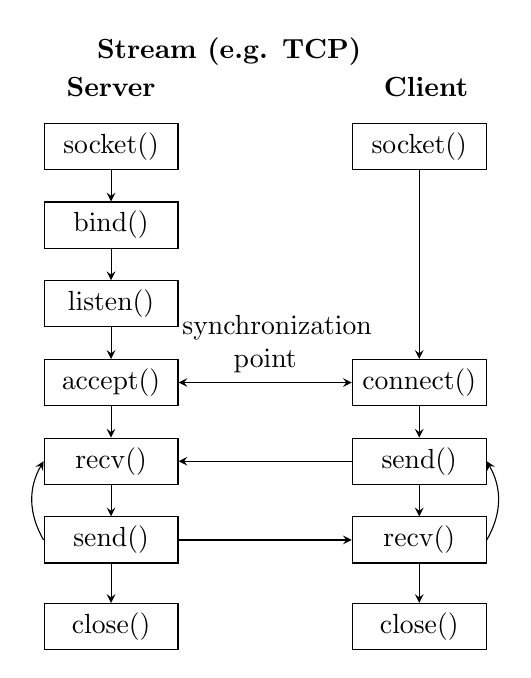
\begin{tikzpicture}
%
% cf. https://latexdraw.com/block-diagram-in-latex-step-by-step-tikz-tutorial/
%
% socket, server
\node [draw,
minimum width=1.7cm,
minimum height=0.4cm]  (serverSocket) at (0, 0) {socket()};

% socket, client
\node [draw,
minimum width=1.7cm,
minimum height=0.4cm,
right=2.2cm of serverSocket]  (clientSocket) {socket()};

% bind, server
\node [draw,
minimum width=1.7cm, 
minimum height=0.4cm,
below=0.4cm of serverSocket
] (serverBind) {bind()};

% listen, server
\node [draw,
minimum width=1.7cm, 
minimum height=0.4cm,
below=0.4cm of serverBind
] (serverListen) {listen()};

% accept, server
\node [draw,
minimum width=1.7cm, 
minimum height=0.4cm,
below=0.4cm of serverListen
] (serverAccept) {accept()};

% connect, client
\node [draw,
minimum width=1.7cm, 
minimum height=0.4cm,
right=2.2cm of serverAccept
] (clientConnect) {connect()};

% recv, server
\node [draw,
minimum width=1.7cm, 
minimum height=0.4cm,
below=0.4cm of serverAccept
] (serverRecv) {recv()};

% send, client
\node [draw,
minimum width=1.7cm, 
minimum height=0.4cm,
right=2.2cm of serverRecv
] (clientSend) {send()};

% send, server
\node [draw,
minimum width=1.7cm, 
minimum height=0.4cm,
below=0.4cm of serverRecv
] (serverSend) {send()};

% recv, client
\node [draw,
minimum width=1.7cm, 
minimum height=0.4cm,
right=2.2cm of serverSend
] (clientRecv) {recv()};


% close, server
\node [draw,
minimum width=1.7cm, 
minimum height=0.4cm,
below=0.5cm of serverSend
] (serverClose) {close()};

% close, client
\node [draw,
minimum width=1.7cm, 
minimum height=0.4cm,
right=2.2cm of serverClose
] (clientClose) {close()};

% Arrows with text label
\draw[-stealth] (serverSocket.south) -- (serverBind.north){};
\draw[-stealth] (serverBind.south) -- (serverListen.north){};
\draw[-stealth] (serverListen.south) -- (serverAccept.north){};
\draw[-stealth] (serverAccept.south) -- (serverRecv.north){};
\draw[-stealth] (serverRecv.south) -- (serverSend.north){};
\draw[-stealth] (serverSend.south) -- (serverClose.north){};

\draw[-stealth] (clientSocket.south) -- (clientConnect.north){};
\draw[-stealth] (clientConnect.south) -- (clientSend.north){};
\draw[-stealth] (clientSend.south) -- (clientRecv.north){};
\draw[-stealth] (clientRecv.south) -- (clientClose.north){};

\draw[-stealth] (clientSend.west) -- (serverRecv.east){};
\draw[-stealth] (serverSend.east) -- (clientRecv.west){};

\draw [-stealth](serverSend.west) to [bend left = 30] (serverRecv.west){};
\draw [-stealth](clientRecv.east) to [bend right = 30] (clientSend.east){};

\draw[stealth-stealth](serverAccept.east) -- (clientConnect.west)
% cf. https://tex.stackexchange.com/questions/228364/is-it-possible-to-set-a-maximum-node-width-in-tikz
node[midway,above, text width=2.1cm, align=center]{synchronization point};

\draw (serverSocket.north)  (0, 1) node[anchor=north] {\textbf{Server}};
\draw (clientSocket.north)  (4, 1) node[anchor=north] {\textbf{Client}};

\draw (serverSocket.north)  (1.5, 1.5) node[anchor=north] {\textbf{Stream (e.g. TCP)}};

\end{tikzpicture}
\qquad \, 
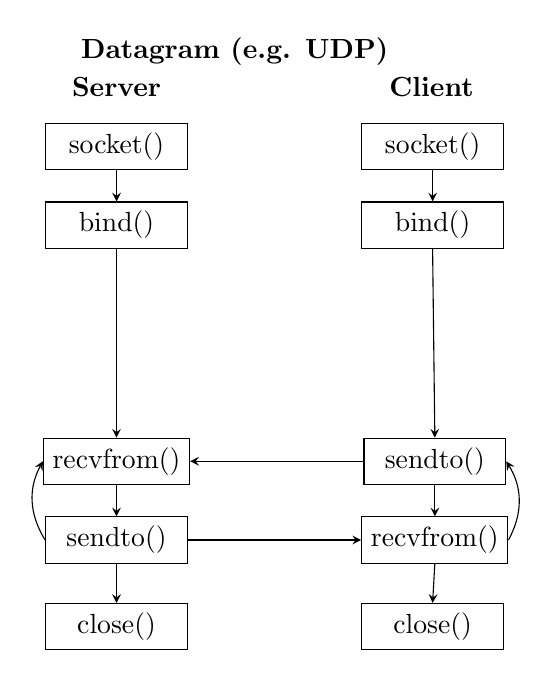
\begin{tikzpicture}
%
% cf. https://latexdraw.com/block-diagram-in-latex-step-by-step-tikz-tutorial/
%
% socket, server
\node [draw,
minimum width=1.8cm,
minimum height=0.4cm]  (serverSocket) at (0, 0) {socket()};

% socket, client
\node [draw,
minimum width=1.8cm,
minimum height=0.4cm,
right=2.2cm of serverSocket]  (clientSocket) {socket()};

% bind, server
\node [draw,
minimum width=1.8cm, 
minimum height=0.4cm,
below=0.4cm of serverSocket
] (serverBind) {bind()};

% bind, client
\node [draw,
minimum width=1.8cm, 
minimum height=0.4cm,
right=2.2cm of serverBind
] (clientBind) {bind()};

% recvfrom, server
\node [draw,
minimum width=1.8cm, 
minimum height=0.4cm,
below=2.4cm of serverBind
] (serverRecvfrom) {recvfrom()};

% sendto, client
\node [draw,
minimum width=1.8cm, 
minimum height=0.4cm,
right=2.2cm of serverRecvfrom
] (clientSendto) {sendto()};

% sendto, server
\node [draw,
minimum width=1.8cm, 
minimum height=0.4cm,
below=0.4cm of serverRecvfrom
] (serverSendto) {sendto()};

% recvfrom, client
\node [draw,
minimum width=1.8cm, 
minimum height=0.4cm,
right=2.2cm of serverSendto
] (clientRecvfrom) {recvfrom()};


% close, server
\node [draw,
minimum width=1.8cm, 
minimum height=0.4cm,
below=0.5cm of serverSendto
] (serverClose) {close()};

% close, client
\node [draw,
minimum width=1.8cm, 
minimum height=0.4cm,
right=2.2cm of serverClose
] (clientClose) {close()};

% Arrows with text label
\draw[-stealth] (serverSocket.south) -- (serverBind.north){};
\draw[-stealth] (serverBind.south) -- (serverRecvfrom.north){};
\draw[-stealth] (serverRecvfrom.south) -- (serverSendto.north){};
\draw[-stealth] (serverSendto.south) -- (serverClose.north){};

\draw[-stealth] (clientSocket.south) -- (clientBind.north){};
\draw[-stealth] (clientBind.south) -- (clientSendto.north){};
\draw[-stealth] (clientSendto.south) -- (clientRecvfrom.north){};
\draw[-stealth] (clientRecvfrom.south) -- (clientClose.north){};

\draw[-stealth] (clientSendto.west) -- (serverRecvfrom.east){};
\draw[-stealth] (serverSendto.east) -- (clientRecvfrom.west){};

\draw [-stealth](serverSendto.west) to [bend left = 30] (serverRecvfrom.west){};
\draw [-stealth](clientRecvfrom.east) to [bend right = 30] (clientSendto.east){};

\draw (serverSocket.north)  (0, 1) node[anchor=north] {\textbf{Server}};
\draw (clientSocket.north)  (4, 1) node[anchor=north] {\textbf{Client}};

\draw (serverSocket.north)  (1.5, 1.5) node[anchor=north] {\textbf{Datagram (e.g. UDP)}};

\end{tikzpicture}
\end{gathered} 
\]
cf. \href{https://www.csd.uoc.gr/~hy556/material/tutorials/cs556-3rd-tutorial.pdf}{CS556 - Distributed Systems, Tutorial by Eleftherios Kosmas, Introduction to Sockets Programming in C using TCP/IP}

cf. \href{https://www.cs.colostate.edu/~massey/Teaching/cs457/}{CS 457, Colorado State, Lecture 20 "Transport Layer: UDP and TCP"}

Recall the application layer is for communication between networked applications. Protocols for application layer include HTTP, FTP, NNTP, etc. \\
Transport layer is for communication between processes (e.g. socket). It relies on network layer and server the application layer. Protocols are TCP and UDP. \\
FYI, network layer is communication between nodes and protocols are IP. \\

So for the \emph{Internet Transport Protocols}, being UDP and TCP, \\
\begin{itemize}
	\item UDP (datagram \emph{messaging} service) 
	\begin{itemize}
		\item No-frills extension of "best-effort" IP
		\item Just send the data - \emph{each send is a message}
	\end{itemize}
	\item TCP (reliable, \emph{streaming}, in-order delivery)
	\begin{itemize}
		\item Connection set-up
		\item Discarding of corrupted packets
		\item Retransmission of lost packets
		\item flow control
		\item congestion control
	\end{itemize}
\end{itemize}

\subsubsection{Multiplexing and Demultiplexing with TCP and UDP}

For the TCP/UDP segment format, the host


\section{References and Resources for Linux System Programming}

\url{http://igm.univ-mlv.fr/~yahya/progsys/linux.pdf} \\
\url{http://www.cs.fsu.edu/~baker/opsys/examples/forkexec/fork_wait.c} \\
\url{http://cs241.cs.illinois.edu/coursebook/}

CS556 - Distributed Systems. Tutorial by Eleftherios Kosmas.
\url{https://www.csd.uoc.gr/~hy556/material/tutorials/cs556-3rd-tutorial.pdf}


\url{https://www.cs.rutgers.edu/~pxk/417/notes/content/02r-sockets-programming-slides.pdf}
\url{https://www.cs.cmu.edu/~srini/15-441/S10/lectures/r01-sockets.pdf}

\url{https://db.in.tum.de/teaching/ss19/c++praktikum/}

\url{https://www.cs.cmu.edu/afs/cs/academic/class/15213-f99/www/class26/}

\part{Networking}

\section{Introduction}

\subsection{Services and Protocols}

cf. 1.5.5 The Relationship of Services to Protocols, Tanenbaum, Feamster, and Wetherall (2021) \cite{TFW2021}

Services and protocols are distinct concepts - this distinction is so important, we emphasize it again.

A \emph{service} is a set of primitives (operations) that a layer provides to the layer above it. \\
- service defines what operations the layer is able to perform on behalf of its users, but says nothing at all about how these operations are implemented. \\

A \emph{protocol} is a set of rules governing the format and meaning of the packets, or messages that are exchanged by peer entities within a layer. Entities use protocols in order to implement their service definitions. They're free to change their protocols at will provided they don't change the service visible to their users. \\
This way, service and protocol are completely decoupled. This is a key concept that any network designer should understand well.

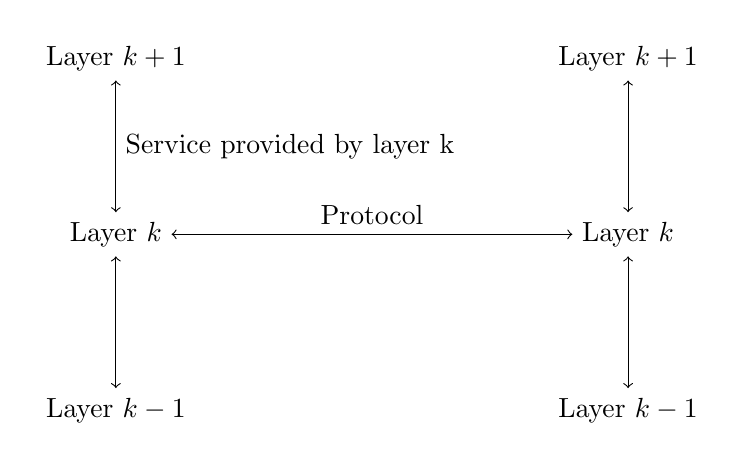
\begin{tikzpicture}
	\matrix (m) [matrix of math nodes, row sep=4.8em, column sep=12.8em, minimum width=1.2em]
	{
		\text{Layer } k + 1 & \text{Layer } k + 1 \\
		\text{Layer } k & \text{Layer } k \\
		\text{Layer } k - 1 & \text{Layer } k - 1 \\
	};
	\path[<->]
	(m-1-1) edge node [right] {\text{Service provided by layer} k} (m-2-1)
	(m-1-2) edge node [left] {} (m-2-2)
	(m-2-1) edge node [left] {} (m-3-1)
	(m-2-2) edge node [left] {} (m-3-2)
	;
	\path[<->]
	(m-2-1) edge node [dashed, above] {\text{Protocol}} (m-2-2)
;
\end{tikzpicture} 

\subsection{Reference Models}

\subsubsection{The OSI Reference Model}

cf. 1.6.1 The OSI Reference Model, Tanenbaum, Feamster, and Wetherall (2021) \cite{TFW2021}

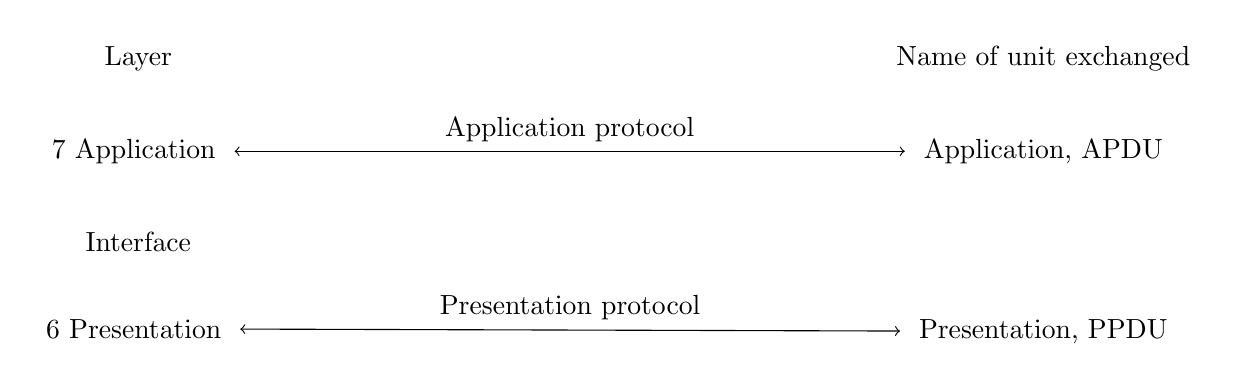
\begin{tikzpicture}
	\matrix (m) [matrix of math nodes, row sep=1.8em, column sep=7.8em, minimum width=1.1em]
	{
		\text{Layer} & & & \text{Name of unit exchanged} \\
		7 \text{ Application } & & & \text{ Application, APDU } \\
		\text{ Interface }  & & &  \\
		6 \text{ Presentation } & & & \text{ Presentation, PPDU } \\
	};
	\path[<->]
	(m-2-1) edge node [dashed, above] {\text{Application protocol} } (m-2-4)
	(m-4-1) edge node [dashed, above] {\text{Presentation protocol}} (m-4-4)
	;
\end{tikzpicture} 

Principles that were applied to arrive at the 7 layers:
\begin{enumerate}
	\item layer should be created where different abstraction is needed
	\item Each layer should perform a well-defined function.
	\item Function of each layer should be chosen with eye toward defining internationally standardized protocols
	\item layer boundaries should be chosen to minimize information flow across the interfaces
	\item number of layers should be large enough that distinct functions need not be thrown together in the same layer out of necessity and small enough that the architecture doesn't become unwieldy.
\end{enumerate}

3 concepts central to OSI model:
\begin{enumerate}
	\item Services
	\item Interfaces
	\item Protocols
\end{enumerate}

\section{Physical Layer}

See Ch. 2 "The Physical Layer", Tanenbaum, Feamster, and Wetherall (2021) \cite{TFW2021}.



\section{Medium Access Control (MAC) Sublayer}

Data link layer or layer 2 is concerned with local delivery of frames between nodes on same level of network; e.g. Ethernet, Point-to-Point Protocol (PPP), HDLC, ADCCP.



\part{C++ Template Metaprogramming}

From this question on \href{https://stackoverflow.com/questions/112277/best-introduction-to-c-template-metaprogramming}{stack overflow}, comes this \href{http://www.cs.rpi.edu/~musser/design/blitz/meta-art.html}{tutorial}. 

cf. Vandevoorde, Josuttis, and Gregor (2017) \cite{VJG2017}. 

\part{Functional Programming and Category Theory}

Best discussion of the relation to monads in category theory to monads in "computer science": \url{https://ncatlab.org/nlab/show/monad+%28in+computer+science%29}

Best article on practical implementation (real daily programming, real programming experiences) of functional programming without pulling punches on Category Theory:

\url{https://nalaginrut.com/archives/2019/10/31/8%20essential%20patterns%20you%20should%20know%20about%20functional%20programming%20in%20c%2B%2B14}

More links:

\url{https://nbviewer.jupyter.org/github/ivanmurashko/articles/blob/master/cattheory/cattheory.pdf}
\url{https://wiki.ifs.hsr.ch/SemProgAnTr/files/mof_categories_final.pdf}

\section{Actors, Concurrent Systems}

\url{https://sourceforge.net/projects/sobjectizer/}
\url{https://github.com/Stiffstream/sobjectizer#helloworld-example}

\v{C}uki\'{c} (2018) \cite{Cuki2018}

Ch. 12, pp. 250, \v{C}uki\'{c} (2018) \cite{Cuki2018}

Consider that multiple (e.g. person) objects shouldn't have any shared data - real people \emph{share} data by \emph{talking} to each other; they don't have shared variables everyone can access and change.

\textbf{actors} - in actor model, actors are completely isolated entities that share nothing but can send messages to 1 another.
\begin{itemize}
	\item actor receives messages and processes them 1 by 1, message $\to$ actor
	\item reaction to message can be change the actor itself or send message to another actor, actor $\to $ another actor in system
\end{itemize}

design actors as follows:

\begin{itemize}
	\item Actors can receive only messages of a signle type, and send messages of a single (not necessarily same) type. If you need to support multiple different types for input or output messages, use \verb|std::variant| or \verb|std::any|, as in Ch. 9, \v{C}uki\'{c} (2018) \cite{Cuki2008}
	\item Leave choice of whom to send message to external controller so can compose actors in a functional way. External controller will schedule which sources an actor should listen to
	\item leave it up to external controller to decide which messages should be processed asynchronously and which shouldn't
\end{itemize}

\url{https://cs.lmu.edu/~ray/notes/messagepassing/} Message passing notes
	
\part{Technical Interviews}

\href{https://classroom.udacity.com/courses/ud513/lessons/7707710408/concepts/77114606610923}{"Interview Introduction", Data Structures and Algorithms in Python, Udacity}

\begin{itemize}
	\item Clarifying the Question
	\item Generating Inputs and Outputs
	\item Generating Test Cases
	\item Brainstorming
	\item Runtime Analysis
	\item Coding
	\item Debugging
\end{itemize}

\section{Puzzles, Brain-teasers}

\url{http://www.mytechinterviews.com/four-people-on-a-rickety-bridge}

20170525 Cyril Zeller, Nvidia had asked this.

Bridge crossing problem. 4 people on 1 side of a bridge. For each A, B, C, D \\
A takes 1 minutes \\
B takes 2 minutes \\
C takes 5 minutes \\
D 10 minutes. \\

At night, only 1 flash light.

No more than 2 people can walk together. Minimize time to cross.

\emph{To reduce the amount of time} find a way for C, D to go together; if they cross together then we need another to come back to get the others. So have a "fast person" like A or B already on the other side. \\

A and B go cross. 2 \\
A or B comes back. 1 \\
C and D go across. 10 \\
B or A comes back. 2 \\
A and B go across (done). \\

Total $ = 2 + 1 + 10 + 2 + 2 = 17$.

\section{Suggested questions to ask the interviewer}

What is the job function? Team? (e.g. what is the function of the team), last is SpaceX itself, What role does this team play in SpaceX?

\section{How to do Code Review}

cf. \href{https://ocw.mit.edu/ans7870/6/6.005/s16/classes/04-code-review/index.html}{6.005, Software Construction, MIT OCW, Reading 4: Code Review}

Core review has 2 purposes:
\begin{itemize}
	\item \textbf{Improving the code}:
	\begin{itemize}
		\item Finding bugs,
		\item anticipating possible bugs,
		\item check clarity of the code,
		\item check consistency with project's style standards
	\end{itemize}
\item \textbf{Improving the programmer}: It's an important way programmers learn and teach each other, about new language features, changes in design of the project or its coding standards, and new techniques
\end{itemize}

Further \href{https://ocw.mit.edu/ans7870/6/6.005/s16/general/code-review.html}{Code review guidelines} for the MIT OCW 6.005 class:

\subsection{Benefits of Code Review}

\begin{itemize}
	\item \emph{Reviewing helps find bugs}, complimentary to other techniques (static checking, testing, assertions, reasoning)
	\item uncovers code that's confusing, poorly documented, unsafe, or otherwise not ready for maintenance or future change
	\item spreads knowledge, allowing developers to learn from each other by explicit feedback and example 
\end{itemize}

\subsection{What to look for}

\textbf{Bugs or potential bugs}
\begin{itemize}
	\item Repetitive code (remember DRY, Don't Repeat Yourself)
	\item Disagreement between code and specification
	\item Off-by-one erros
	\item Global variables, and other too-large variable scopes
	\item optimistic, undefensive programming
	\item magic numberes
	\item \dots (other)
\end{itemize}

\textbf{Unclear, messy code}
\begin{itemize}
	\item Bad variable or method names, 
	\item Inconsistent indentation
	\item Convoluted control flow (if and while statements) that could be simplified
	\item Packing too much into one line of code, or too much into 1 method
	\item Failing to comment obscure code.
	\item Having too many trivial comments that are simply redundant with the code
	\item Variables used for more than 1 purpose.
	\item \dots (other)
\end{itemize}

\textbf{Misusing (or failing to use) essential design concepts}
\begin{itemize}
	\item Incomplete or incorrect specification for a method or class,
	\item representation exposure for a data abstraction,
	\item Immutable datatypes that expose themselves to change,
	\item invariants that aren't really invariant, or aren't even stated
\end{itemize}

Positive comments are good; don't be afraid to make comments about things you really like, e.g.:
\begin{itemize}
	\item \textbf{Unusually elegant code}
	\item \textbf{Creative solutions}
	\item \textbf{Great design}
\end{itemize}

\subsubsection{Respect in Code Review}
\textbf{Be polite}. \\
\textbf{Be constructive}. Don't just criticize, but be helpful: point the way toward solutions.

\subsubsection{Further FAQ}

\textbf{I don't feel like I know anything. How can I possibly review other people's code?} You know more than you think you do. You can read for clarity, comment on places where the code is confusing, look for problems we read about, know about, talked about, etc.

\textbf{What if I can't find anything wrong?} You can write a specific positive comment about something good.


\subsubsection{On Style, Style Standards}

cf. \href{https://ocw.mit.edu/ans7870/6/6.005/s16/classes/04-code-review/index.html}{Reading 4: Code Review, Software in 6.005}

It's \emph{very} important to follow the conventions of the project. For instance, if you're the programmer who reformats every module you touch to match your personal style, your teammates will hate you, and rightly so. Be a team player.

\subsubsection{Smelly Example 1}

Programmers often describe bad code as having a "bad smell" that needs to be removed.

\begin{verbatim}
public static int dayOfYear(int month, int dayOfMonth, int year) {
if (month == 2) {
dayOfMonth += 31;
} else if (month == 3) {
dayOfMonth += 59;
} else if (month == 4) {
dayOfMonth += 90;
} else if (month == 5) {
dayOfMonth += 31 + 28 + 31 + 30;
} else if (month == 6) {
dayOfMonth += 31 + 28 + 31 + 30 + 31;
} else if (month == 7) {
dayOfMonth += 31 + 28 + 31 + 30 + 31 + 30;
} else if (month == 8) {
dayOfMonth += 31 + 28 + 31 + 30 + 31 + 30 + 31;
} else if (month == 9) {
dayOfMonth += 31 + 28 + 31 + 30 + 31 + 30 + 31 + 31;
} else if (month == 10) {
dayOfMonth += 31 + 28 + 31 + 30 + 31 + 30 + 31 + 31 + 30;
} else if (month == 11) {
dayOfMonth += 31 + 28 + 31 + 30 + 31 + 30 + 31 + 31 + 30 + 31;
} else if (month == 12) {
dayOfMonth += 31 + 28 + 31 + 30 + 31 + 30 + 31 + 31 + 30 + 31 + 31;
}
return dayOfMonth;
}
\end{verbatim}

\subsubsection{Don't Repeat Yourself}

Duplicated code is a risk to safety. If you have identical or very similar code in 2 places, then the fundamental risk is there's a bug in both copies, and some maintainer fixes the bug in 1 place, but not the other.

EY: If you're doing the same computation, with small change, consider defining it in another place.

\subsubsection{Comments Where Needed}

Good comments should make code easier to understand, safer from bugs (because important assumptions have been documented), and ready for change.

One kind of crucial comment is a \emph{specification}, which appears above a method or above a class and documents the behavior of the method or class.

Specifications document assumptions. 

Another crucial comment is one that specifies the provenance or source of a piece of code that was copied or adapted from elsewhere. 

For example,

\begin{verbatim}
// read a web page into a string
// see http://stackoverflow.com/questions/4328711/read-url-to-string-in-few-lines-of-java-code
String mitHomepage = new Scanner(new URL("http://www.mit.edu").openStream(), "UTF-8").useDelimiter("\\A").next();
\end{verbatim}

One reason for documenting sources is to avoid copyright violations. Also another is that code can fall out of date; a Stack Overflow answer from which code came from could have evolved significantly since the years it was first answered.

Some comments are bad and unnecessary. For instance, direct transliterations of code into English do nothing to improve understanding., e.g.

\begin{verbatim}
while (n != 1) { // test whether n is 1   (don't write comments like this!)
++i; // increment i
l.add(n); // add n to l
}
\end{verbatim}

But obscure code should get a comment:
\begin{verbatim}
sendMessage("as you wish"); // this basically says "I love you"
\end{verbatim}

\subsubsection{Fail Fast}

\emph{Failing fast} means code should reveal its bugs as early as possible. 

For instance, static checking fails faster than dynamic checking, and dynamic checking fails faster than producing a wrong answer that may corrupt subsequent computation.

In the \verb|dayOfYear| example, there should be static checking of input arguments, because if you pass arguments in wrong order, it'll quietly return the wrong answer.

\subsubsection{Avoid Magic Numbers}

\subsubsection{Don't Use Global Variables}

Avoid global variables.

In Java, \verb|static| means there's a single instance of the variable.

In general, change global variables into parameters and return values, or put them inside objects that you're calling methods on.


\subsection{Summary for Code Review}

\begin{itemize}
	\item Don't Repeat Yourself (DRY)
	\item Comments where needed
	\item Fail fast
	\item Avoid magic numbers
	\item One purpose for each variable
	\item Use good names
	\item No global variables
	\item Use whitespace for readability
\end{itemize}

\part{Embedded Systems}

Lee and Seshia (2016) \cite{LeSe2016}.

cf. Ch. 3 Discrete Dynamics, Lee and Seshia (2016) \cite{LeSe2016}. 

showed how state machines can be used to model discrete dynamics.

cf. Sec. 3.1., Lee and Seshia (2016) \cite{LeSe2016}. 

pp. 43, Ex. 3.1., Lee and Seshia (2016) \cite{LeSe2016}. e.g. Consider system that counts number of cars that enter and leave parking garage in order to keep track of how many cars are in garage at any time. 

Ignore for now how to design sensors that detect entry or departure of cars.

Assume \texttt{ArrivedDetector} actor produces an event when car arrives, and \texttt{DepartureDetector} actor produces an event when car departs.

\texttt{Counter} actor keeps running count, starting from initial value $i$. 

Each time count changes, it produces an output event that updates display.

Each entry or departure modeled as \textbf{discrete event}. Discrete event \textbf{occurs at} an instant of time rather than over time.

EY: So there are \emph{3} actors:

\begin{enumerate}
	\item Arrival Detector $\to$ produces event when car arrives
	\item Departure Detector $\to$ produces event when car departs
	\item Counter actor (keeps running count, each time count changes (so it's a FSM)) -> produces output event that updates a display
\end{enumerate}

Signal $u$ into \texttt{up} input port (from \texttt{ArrivalDetector}, upon arrival) is function of form
\[
u : \mathbb{R} \to \lbrace \text{absent}, \text{present} \rbrace, \text{ i.e. }
\]

$\forall \, $ time $t\in \mathbb{R}$, $u(t) $ either absent, i.e. there's no event at that time, or present, meaning there is a \\

\textbf{pure signal} - signal or function of form $u:\mathbb{R} \to \lbrace \text{ absent, present} \rbrace$, carries no value, but instead provides all its information by either being present or absent at any given time. \\

Counter: when \textbf{event} is present at up input port, increment count and produce output of new count value. \\
When event present at down input, decrements count and produces output new count value. \\
At other times, produces no output (count output is absent) \\

Hence, 
\[
c: \mathbb{R} \to \lbrace \text{ absent } \rbrace \bigcup \mathbb{Z}
\]
Counter signal is not pure. \\

Input to counter is pair of discrete signals that at certain times have an event, at other times have no event. Output is also discrete signals. \\

signals $\xrightarrow{ \text{ counter } }$ output signal \\

EY: separate FSM logic from this signal or message passing function.


\begin{definition}[Signal and discrete signal]
	Signal is a function of the form $e : \mathbb{R} \to \lbrace \text{absent}  \rbrace \bigcup X, \, X \in \text{Obj}{\mathbf{Set}}$ s.t. \\
	$\exists \,$ 1-to-1 $f: T \to \mathbb{N}$, s.t. $f$ order preserving, i.e. $\forall \, t_1, t_2 \in T$, if $t_1 \leq t_2$, then $f(t_1) \leq f(t_2)$, where $T = T_{\text{present}} = \lbrace t \in \mathbb{R} | e(t) \neq \text{absent} \rbrace$.

	$e$ is \textbf{discrete} if $\exists \,$ 1-to-1 $f:T\to \mathbb{N}$ such that $f$ order preserving.
\end{definition} 

pp. 46, Sec. 3.1 Discrete Systems, Lee and Seshia (2016) \cite{LeSe2016}, \\
dynamics of discrete system can be described as sequence of steps called \textbf{reactions}. \\
Assume reactions instantaneous. \\
reactions of discrete system triggered by environment which discrete system operates. e.g. Fig. 3.1, reactions of counter actor triggered when 1 or more input events present. \\
$\to$ reactions are \textbf{event-triggered} in this case.

\subsection{Modeling Actors as Functions}

Integrator actor (cf. Sec.2.2, Fig. 3.2):
\[
\begin{gathered}
\begin{aligned}
& I_i : \mathbb{R}^{\mathbb{R}^+} \to \mathbb{R}^{\mathbb{R}^+}, \, \text{ i.e. } \\
& I_i : (\mathbb{R}^+ \to \mathbb{R}) \to (\mathbb{R}^+ \to \mathbb{R})
\end{aligned}\\
y = I_i(x)
\end{gathered}
\]

where $i\equiv $ initial value of integration, $x,y$ are cont.-time signals; \\
e.g. if $i=0$, and $\forall \, t \in \mathbb{R}^+$, $x(t) = 1$, then 
\[
y(t) = i + \int_0^t x(\tau) d\tau = t
\]

Fig. 3.1, Counter modeled by
\[
C_i: (\mathbb{R}^+ \to \lbrace \text{absent}, \text{present} \rbrace)^P \to (\mathbb{R}^+ \to \lbrace \text{absent} \bigcup \mathbb{Z})
\]
where $P = $ set of inputs or input ports. \\

Recall $A^B \equiv$ set of all functions from $B$ to $A$. \\

Input to function $C$ is function whose domain is $P$ that $\forall \, $ port $p\in P$ yields function in $(\mathbb{R}^+ \to \lbrace \text{ absent , present } \rbrace )$, i.e.

\[
C_i: \text{Hom}( \text{Hom}(\mathbb{R}^+ , \lbrace \text{absent, present} \rbrace )) \to \text{Hom}(\mathbb{R}^+, \lbrace \text{ absent } \bigcup \mathbb{Z} )
\]

Suppose actor has input ports $P = \lbrace p_1, \dots p_N \rbrace$ where $p_i \equiv $ name of $i$th input port. \\

Assume $\forall \, $ input port $p\in P$, set $V_p$ denotes values that may be received on port $p$ when input present; $V_p \equiv$ called \textbf{type} of port $p$. \\
At reaction, treat each $p \in P$ as variable that takes $p\in V_P \bigcup \lbrace \text{ absent } \rbrace$. \\
\textbf{valuation} of inputs $P$ is assignment of value in $V_P$\, $\forall \, p \in P$ or assertion that $p$ absent. \\
If port $p$ receives pure signal, then $V_p = \lbrace \text{ present } \rbrace$. \\

Example 3.2. For garage counter, set of input ports $P = \lbrace \text{ up, down } \rbrace$. Both receive pure signals, so $V_{\text{up}} = V_{\text{down}} = \lbrace \text{ present } \rbrace$. If car is arriving at time $t$ and none departing, then at reaction, $\text{up}(t) = $ present, $\text{down}(t) = $ absent. \\

\subsubsection{Outputs}

output ports $Q = \lbrace q_1, \dots q_M \rbrace$ with types $V_{q_1}, \dots V_{q_m}$. \\
At each reaction, system assigns value $q\in V_q \bigcup \lbrace \text{absent} \rbrace \, \forall \, q \in Q$, producing a valuation of outputs. \\

Example 3.3. Counter actor, Fig. 3.1, 1 output port named count, so $Q = \lbrace \text{ count } \rbrace$, type $V_{\text{count}} = \mathbb{Z}$, at reaction, count is assigned count of cars in garage.

EY: Lee and Seshia (2016) \cite{LeSe2016} fails to model the Arrival Detector and Departure Detector actors, which should not carry state because state is not required to modeled its behavior. Also, if Lee and Seshia claim that ArrivalDetector and DepartureDetector actors are \emph{event-driven}, as strongly implied by the fact that they produce events when car arrives or departs respectively, and those events become the input signals to Counter, then the inputs into their "ports" aren't necessarily of the form $\lbrace \text{absent, present} \rbrace$, nor $\text{Hom}(\mathbb{R}^+, \lbrace \text{absent, present} \rbrace)$. It could be much simpler. 

cf. pp. 52 Lee and Seshia (2016) \cite{LeSe2016}

For example, in Figure 3.5, for the thermostat with hysteresis (so that it avoids \textbf{chattering}, heater would turn on and off rapidly when temperature is close to setpoint temperature), the finite state machine (FSM) could be \textbf{event triggered}, like the garage counter, in which case it'll react whenever a \emph{temperature} input is provided.

Alternatively, it could be \textbf{time triggered} - it reacts at regular time intervals.

The definition of FSM doesn't change in these two cases: it's up to the environment in which an FSM operates when it should react.

cf. pp. 52, Sec. 3.3.2 "When a Reaction Occurs", Lee and Seshia (2016) \cite{LeSe2016}

Recall the notion of "reaction": from pp. 48, Sec. 3.2 "The Notion of State", formally define state to be encoding of everything about past that has an effect on system's reaction to current or future inputs. From Sec. 3.3 "Finite-State Machines", 
\begin{definition}[State Machine, Sec. 3.3 Finite State Machines, Lee and Seshia (2016)\cite{LeSe2016}, pp. 48]
	\textbf{state machine} is a model of a system with discrete dynamics that at each \emph{reaction} maps valuations of inputs to valuations of outputs, where map may depend on its current state.
	\textbf{finite-state machine} (FSM) is a state machine where the set \emph{States} of possible states is finite.
\end{definition}

However, \emph{nothing in the definition of a state machine constrains \textbf{when} it reacts}. The environment determines when machine reacts. Chapters 5, 6 of Lee and Seshia (2016) \cite{LeSe2016} describe a variety of mechanisms and give precise meaning to terms like \textbf{event triggered} and \textbf{time triggered}.

cf. Sec. 3.4 Extended State Machines, Lee and Seshia (2016) \cite{LeSe2016}

Pushes problem of large number of states into a variable, and there's only 1 state.

e.g. garage counter of Fig. 3.4, in Fig. 3.8

pp. 62, "Extended state machines can provide a convenient way to keep track of the passage of time." but merely pushes tracking time to input variable. e.g. Ex. 3.9, traffic light, Fig. 3.10. \\

Lee and Seshia mixes extended state machine state with discrete state and variables; but variables act as input.

Sec. 3.5 Nondeterminism, Fig. 3.11 nondeterministic model of pedestrians (as FSM)

state machine nondeterministic if more than 1 initial state (sufficient condition) or \\
if $\forall \,$ state, $\exists !$ 2 distinct transitions with guards that can evaluate to true in same reaction \\

\part{Design}

cf. Daniel Jackson. 6.170 Software Studio. Spring 2013. Massachusetts Institute of Technology: MIT OpenCourseWare, \url{https://ocw.mit.edu}. License: Creative Commons BY-NC-SA. \cite{Jack2013}

\section{System Design}

\subsection{Client-Server}

Let (notation) \\
client $\equiv \text{cli}$, \\
server $\equiv \text{ser}$, \\

$\text{cli}$ actions : $\lbrace $ request data, speak to $\text{ser} \rbrace$  \\
$\text{ser}$ actions: $\lbrace$ listen, send data $\rbrace$ \\

$\text{cli}$ action: make DNS query. Obtain IP address. \\

e.g. $\text{cli} \equiv $ browser. \\
browser makes DNS query. gets back IP address. \\
IP address $\equiv $ unique identifier for machine on network and internet. \\

$\text{cli}$ http request $\to  \text{ser}$ \\

$\text{ser}$ listen to requests on ports $\sim 16000$ ports. \\
Need to specify port. \\
For http, port 80, https port 443 (decided upon long time ago). \\

Try the following:

\begin{lstlisting}
dig algoexpert.io
dig google.com

nc -l 8081 # l for listen
nc 127.0.0.1 # 127.0.0.1 for local machine
\end{lstlisting}

\subsection{Relational Databases}

Structure imposed on data. \\
2 (major) structures. \\
Relational Databases (Db's) vs. Non-relational Db's \\
Tables or relations \\
columns represent attributes \\
rows referred to often as records. \\

Non-relational Db's.

SQL - structured query.

\subsubsection{SQL query (time complexity)}

$O(1)$ - hash index on id, or cached result on id from previous query. \\
$O(n)$ - Do full scan and look at each row; \\
$O(\log{(n)})$ sort id and do binary search. \\

cf. \url{https://www.geeksforgeeks.org/sql-query-complexity/}

\subsubsection{Databases definition}

Databases (db) uses disk or memory for 2 actions: record data, query data. \\
In general, they're themselves servers that are long lived and interact with rest of application through network calls, with protocols on top of TCP or even HTTP. 

Some db's keep records in memory, users of such db's are aware records maybe lost forever if machine or process dies.


\subsection{Example: Payments, payments processing system}

Payment design. \\
Users authorize payments, system interfaces with external payment processes like Visa to copmlete payment. \\
Queue based architecture. \\
Payment systems demand high reliability. Not making payments users requested or charging users multiple times - consequences too high. 

To achieve this reliability, system puts "payment task" onto a queue that's processed asynchronously.

\begin{enumerate}
	\item user $u$. action, payment request. front-end service accepts $u$'s payment request. \\
	Set up record in database that says $u$'s request, says status request received, payment pending. \\
	record will be used to communicate with user what states of payment is. \\
	front-end service $\equiv s_{fr}$. $s_{fr}$ has action accepts, accepts $ : u$
	\item $s_{fr}$ has action put message on payment queue. \\
	message has information: reference to newly created database record, details about payment (which credit card to use, amount, etc.) \\
	If either step or previous one failed, user immediately notified. 
	\item asynchronous processor reads from queue, process individual payments. \\
	primary objective if the processing is to make the payment using external payment service (like Visa) and update $u$'s payment database record based on result.
	\item Once payment goes through or fails in nonrecoverable way (e.g. external service rejects payment due to insufficient funds), asynchronous processor notifies user.
\end{enumerate}

cf. \url{https://www.linkedin.com/pulse/system-design-practice-designing-payment-avik-das/}


\end{multicols*}

\begin{thebibliography}{9}

\bibitem{BrOH2016}
Randal E. Bryant, David R. O'Hallaron. \textbf{Computer Systems: A Programmer's Perspective} (3rd Edition). ISBN-13 : 978-0134092669
ISBN-10 : 013409266X
 Pearson; 3rd Edition (March 12, 2015) 
\url{https://csapp.cs.cmu.edu/}


\bibitem{Meye1997}
Bertrand Meyer. \textbf{Object-Oriented Software Construction} (Book/CD-ROM) (2nd Edition) 2nd Edition.   Prentice Hall; 2 edition (April 13, 1997).  ISBN-13: 978-0136291558

\bibitem{Hyde2004}
Randall Hyde.  \textbf{Write Great Code: Volume 1: Understanding the Machine} October 25, 2004.  No Starch Press; 1st edition (October 25, 2004).  ISBN-13: 978-1593270032

\bibitem{Hyde2006}
Randall Hyde.  \textbf{Write Great Code, Volume 2: Thinking Low-Level, Writing High-Level}.   1st Edition.  No Starch Press; 1 edition (March 18, 2006).  ISBN-13: 978-1593270650

\bibitem{Shaw2015}
Zed A. Shaw.  \textbf{Learn C the Hard Way: Practical Exercises on the Computational Subjects You Keep Avoiding (Like C)} (Zed Shaw's Hard Way Series) 1st Edition.  Addison-Wesley Professional; 1 edition (September 14, 2015) ISBN-13: 978-0321884923.  

\bibitem{Bend}
Eli Bendersky.   \href{https://eli.thegreenplace.net/2009/10/21/are-pointers-and-arrays-equivalent-in-c}{Are pointers and arrays equivalent in C?}

\bibitem{KeRi1988}
Brian W. Kernighan, Dennis M. Ritchie.  \textbf{C Programming Language}, 2nd Ed. 1988.   

\bibitem{Vand1994}
Peter van der Linden.  \textbf{Expert C Programming: Deep C Secrets} 1st Edition.  Prentice Hall; 1st edition (June 24, 1994)  ISBN-13: 978-0131774292

\bibitem{Ferr2010}
Leo Ferres.  "Memory management in C: The heap and the stack".  \href{http://www.inf.udec.cl/~leo/teoX.pdf}{Memory management in C: The heap and the stack}


\bibitem{Stro2013}
Bjarne Stroustrup.  \textbf{The C++ Programming Language}, 4th Edition. Addison-Wesley Professional; 4 edition (May 19, 2013).  ISBN-13: 978-0321563842

\bibitem{Gott2015}
Peter Gottschling. \textbf{Discovering Modern C++: An Intensive Course for Scientists, Engineers, and Programmers (C++ In-Depth Series)}. Addison-Wesley Professional; 1st edition (December 17, 2015). ISBN-10 : 0134383583
ISBN-13 : 978-0134383583 

\bibitem{GhJa1997} 
Carlo Ghezzi, Mehdi Jazayeri.  \textbf{Programming Language Concepts} 3rd Edition.  Wiley; 3 edition (June 23, 1997).  ISBN-13: 978-0471104261  \url{https://vowi.fsinf.at/images/7/72/TU_Wien-Programmiersprachen_VL_(Puntigam)_-_E-Book_SS08.pdf}

\bibitem{LLM2012}
Stanley B. Lippman, Jos\'{e}e Lajoie, Barbara E. Moo. \textbf{C++ Primer} (5th Edition).  Addison-Wesley Professional; 5 edition (August 16, 2012) ISBN-13: 978-0321714114 

\bibitem{ScMe2014}
Scott Meyers.  \textbf{Effective Modern C++: 42 Specific Ways to Improve Your Use of C++11 and C++14}. 1st Edition.  O'Reilly Media; 1 edition (December 5, 2014)  ISBN-13: 978-1491903995

\bibitem{BGG2016}
Ana Bell, Eric Grimson, and John Guttag. \emph{6.0001 Introduction to Computer Science and Programming in Python}. Fall 2016. Massachusetts Institute of Technology: MIT OpenCourseWare, \url{https://ocw.mit.edu}. License: Creative Commons BY-NC-SA.


\bibitem{DeDe2001}
Erik Demaine, and Srini Devadas. 6.006 Introduction to Algorithms. Fall 2011. Massachusetts Institute of Technology: MIT OpenCourseWare, \url{https://ocw.mit.edu}. License: Creative Commons BY-NC-SA.

\bibitem{Hard2018}
Douglas Wilhelm Harder, M.Math. LEL. ECE 250 \emph{Algorithms and Data Structures}. Waterloo Engineering. Department of Electrical and Computer Engineering. University of Waterloo. Waterloo, Ontario, Canada. \url{https://ece.uwaterloo.ca/~dwharder/aads/Lecture_materials/#introduction-and-reveiew}

\bibitem{Diet2019}
Martin Dietzfelbinger. Algorithmen und Datenstrukturen 1 - WS 19/20. FG KtuEA, TU Ilmenau. Oktober 2019. Technische Universit\"{a}t Ilmenau. Fakult\"{a}t f\"{u}r Informatik und Automatisierung. \href{https://www.tu-ilmenau.de/en/institute-of-theoretical-computer-science/lehre/lehre-ws-20192020/aud-1/}{Algorithmen und Datenstrukturen 1, WS 19/20}


\bibitem{CLRS2009}
Thomas H. Cormen, Charles E. Leiserson, Ronald L. Rivest and Clifford Stein.  \textbf{Introduction to Algorithms}, \emph{Third Edition}. MIT Press; Sept. 1, 2009.  ISBN-13 : 978-0262033848 

\href{https://walkccc.me/CLRS/}{Solutions to Introduction to Algorithms Third Edition}

\bibitem{CLRS2022}
Thomas H. Cormen, Charles E. Leiserson, Ronald L. Rivest and Clifford Stein.  \textbf{Introduction to Algorithms}, \emph{Fourth Edition}. MIT Press; April 2022.

\bibitem{SeWa2011}
Robert Sedgewick and Kevin Wayne. \textbf{Algorithms}. 4th Edition. Addison-Wesley Professional; 4th edition (April 3, 2011). ISBN-10 : 032157351X
ISBN-13 : 978-0321573513 

\bibitem{Shaf2011}
Dr. Clifford A. Shaffer. \textbf{Data Structures and Algorithm Analysis in C++}, Third Edition (Dover Books on Computer Science) Third Edition. Dover Publications; (September 14, 2011). ISBN-10 : 048648582X ISBN-13 : 978-0486485829 


\bibitem{Neag2020}
\href{https://www.udemy.com/course/master-the-coding-interview-data-structures-algorithms/#instructor-1}{Andrei Neagole}. Master the Coding Interview: Data Structures $+$ Algorithms. 
\url{https://www.udemy.com/course/master-the-coding-interview-data-structures-algorithms/}

\bibitem{Fuss2011}
Prof. Donald S. Fussell (Instructor). CS429H (378H) - Systems I (Honors) (Computer Organization, Architecture, and Programming). Spring 2011. University of Texas. \url{https://www.cs.utexas.edu/users/fussell/courses/cs429h/}

\bibitem{Srid2017} Cindy Sridharan. "The method to epoll's madness." \emph{Medium}. Oct. 29, 2017. \url{https://medium.com/@copyconstruct/the-method-to-epolls-madness-d9d2d6378642}

\bibitem{TFW2021}
Andrew S. Tanenbaum. Nick Feamster. David Wetherall. \textbf{Computer Networks}. Sixth Edition. Global Edition. Pearson. 2021. ISBN 13: 978-1-292-37406-2.

\bibitem{VJG2017}
David Vandevoorde, Nicolai M. Josuttis, Douglas Gregor. \textbf{C++ Templates: The Complete Guide} (2nd Edition). Addison-Wesley Professional; 2 edition (September 18, 2017). ISBN-13: 978-0321714121

\bibitem{Cuki2018}
Ivan \v{C}uki\'{c}. \textbf{Functional Programming in C++: How to improve your C++ programs using functional techniques}. 1st Edition. 2018


\bibitem{LeSe2016}
Edward Ashford Lee, Sanjit Arunkumar Seshia. \textbf{Introduction to Embedded Systems: A Cyber-Physical Systems Approach} (The MIT Press) Second Edition. The MIT Press; Second edition (December 30, 2016). ISBN-10: 0262533812. ISBN-13: 978-0262533812

\bibitem{Gutt2016}
John V. Guttag. \textbf{Introduction to Computation and Programming Using Python (With Application to Understanding Data)}. 2nd Edition. 	MIT Press.  ISBN-13 : 978-0262529624 

\bibitem{6dot005and6dot031}
\textbf{6.005: Software Construction}, \textbf{6.031: Software Construction}. \href{http://web.mit.edu/6.031/www/sp20/}{6.031: Software Construction, Spring 2020}: Max Goldman, Rob Miller.


\bibitem{Jack2013}
Daniel Jackson. \emph{6.170 Software Studio}. Spring 2013. Massachusetts Institute of Technology: MIT OpenCourseWare, \url{https://ocw.mit.edu}. License: Creative Commons BY-NC-SA.

\bibitem{Kerr2010}
Michael Kerrisk. \textbf{The Linux Programming Interface: A Linux and UNIX System Programming Handbook}. No Starch Press; 1st edition (October 28, 2010). ISBN-10 : 1593272200 ISBN-13 : 978-1593272203 

\bibitem{SFR2004}
W. Richard Stevens, Bill Fenner, Andrew M. Rudoff. \textbf{UNIX Network Programming: The Sockets Networking API}. Volume 1. Third Edition. 2004. ISBN: 0-13-141155-1


\end{thebibliography}

\end{document}



